% =====================================================================
%  RELATÓRIO TÉCNICO DE CICLO DE PROJETO
%  Tópicos em Sistemas Computacionais I (IoT/AIoT) · UFPI · 2026.2
%
%  COMO USAR
%  1. Abra config/dados-da-equipe.tex e preencha. É o único arquivo de
%     configuração que vocês precisam tocar.
%  2. Escreva nos arquivos da pasta conteudo/, na ordem em que aparecem
%     abaixo. Cada um começa com uma caixa cinza explicando o que vai ali.
%  3. Preencha os apêndices A e B com o mapa de barramento (Aula 06) e o
%     orçamento de energia (Aula 08) que a equipe já entregou. Na AP2,
%     os apêndices E e F (checklist e campanha) aparecem sozinhos.
%  4. Antes de entregar, comente a linha \def\MOSTRARNOTAS{} em
%     config/dados-da-equipe.tex para sumir com as caixas de instrução.
%  5. Compile duas vezes, rode o BibTeX e compile mais duas.
%     No Overleaf: basta apertar Recompile (ele faz isso sozinho).
% =====================================================================

\documentclass[
  12pt,
  oneside,
  a4paper,
  sumario=tradicional,
  english,
  brazil
]{abntex2}

% =====================================================================
%  config/pacotes.tex
%  Pacotes e configuracao de aparencia. Voce nao precisa mexer aqui.
% =====================================================================

% --- Codificacao e fontes ---------------------------------------------
\usepackage[T1]{fontenc}
\usepackage[utf8]{inputenc}
\usepackage{lmodern}
\usepackage{microtype}
\usepackage{csquotes}

% --- Graficos, cores e caixas -----------------------------------------
\usepackage{graphicx}
\usepackage{xcolor}
\usepackage{float}
\usepackage[most]{tcolorbox}

% --- Tabelas ----------------------------------------------------------
\usepackage{booktabs}
\usepackage{array}
\usepackage{tabularx}
\usepackage{longtable}
\usepackage{multirow}
\usepackage{makecell}
\usepackage{pdflscape}

% --- Listas, unidades, matematica -------------------------------------
\usepackage{enumitem}
\usepackage{amsmath}
\usepackage{amssymb}
\usepackage{siunitx}
\sisetup{
  output-decimal-marker = {,},
  group-separator       = {.},
  group-minimum-digits  = 4,
  per-mode              = symbol,
  detect-weight         = true,
}
\DeclareSIUnit{\mAh}{mA\cdot h}
\DeclareSIUnit{\Wh}{W\cdot h}
\DeclareSIUnit{\HSP}{HSP}
\DeclareSIUnit{\baud}{Bd}

% --- Codigo-fonte -----------------------------------------------------
\usepackage{listings}
\definecolor{corComentario}{HTML}{4F7942}
\definecolor{corPalavra}{HTML}{0B3D91}
\definecolor{corTexto}{HTML}{8B1A1A}
\definecolor{corFundo}{HTML}{F7F7F7}
\definecolor{corRegua}{HTML}{BFBFBF}
\definecolor{corDestaque}{HTML}{0B3D91}

\lstset{
  basicstyle        = \ttfamily\footnotesize,
  keywordstyle      = \color{corPalavra}\bfseries,
  commentstyle      = \color{corComentario}\itshape,
  stringstyle       = \color{corTexto},
  numbers           = left,
  numberstyle       = \ttfamily\scriptsize\color{corRegua},
  numbersep         = 8pt,
  backgroundcolor   = \color{corFundo},
  frame             = single,
  rulecolor         = \color{corRegua},
  breaklines        = true,
  breakatwhitespace = true,
  showstringspaces  = false,
  tabsize           = 2,
  captionpos        = b,
  extendedchars     = true,
  inputencoding     = utf8,
  literate =
    {á}{{\'a}}1 {é}{{\'e}}1 {í}{{\'i}}1 {ó}{{\'o}}1 {ú}{{\'u}}1
    {Á}{{\'A}}1 {É}{{\'E}}1 {Í}{{\'I}}1 {Ó}{{\'O}}1 {Ú}{{\'U}}1
    {à}{{\`a}}1 {À}{{\`A}}1
    {â}{{\^a}}1 {ê}{{\^e}}1 {ô}{{\^o}}1
    {Â}{{\^A}}1 {Ê}{{\^E}}1 {Ô}{{\^O}}1
    {ã}{{\~a}}1 {õ}{{\~o}}1 {Ã}{{\~A}}1 {Õ}{{\~O}}1
    {ç}{{\c c}}1 {Ç}{{\c C}}1
    {°}{{\textdegree}}1 {º}{{\textordmasculine}}1 {ª}{{\textordfeminine}}1
    {Ω}{{\ensuremath{\Omega}}}1 {µ}{{\ensuremath{\mu}}}1
    {·}{{\textperiodcentered}}1
}

% Linguagem para o firmware do ESP32 (C/C++ estilo Arduino)
\lstdefinestyle{arduino}{
  language  = C++,
  morekeywords = {setup, loop, pinMode, digitalWrite, digitalRead,
                  analogRead, analogWrite, delay, millis, micros,
                  Serial, Wire, SPI, uint8_t, uint16_t, uint32_t,
                  int8_t, int16_t, int32_t, esp_deep_sleep_start,
                  esp_sleep_enable_timer_wakeup, RTC_DATA_ATTR,
                  HIGH, LOW, INPUT, OUTPUT, INPUT_PULLUP, true, false},
}
\lstdefinestyle{terminal}{
  language     = bash,
  numbers      = none,
  basicstyle   = \ttfamily\footnotesize,
  keywordstyle = \color{corPalavra},
}

% --- Referencias cruzadas e links -------------------------------------
\usepackage[brazilian,hyperpageref]{backref}
\usepackage[alf]{abntex2cite}

\renewcommand{\backrefpagesname}{Citado na(s) pagina(s):~}
\renewcommand{\backref}{}
\renewcommand*{\backrefalt}[4]{%
  \ifcase #1 %
    Nenhuma citacao no texto.%
  \or
    Citado na pagina #2.%
  \else
    Citado #1 vezes nas paginas #2.%
  \fi}

% =====================================================================
%  config/dados-da-equipe.tex
%  ESTE É O ÚNICO ARQUIVO DE CONFIGURAÇÃO QUE A EQUIPE PRECISA EDITAR.
%  Leva dois minutos. Faça isso antes de escrever qualquer coisa.
% =====================================================================

% --- 1. Qual ciclo de projeto este relatório documenta? ---------------
%     1 = AP1 (sensoriamento e atuação)
%     2 = AP2 (conectividade e conjunto de dados)
%     3 = AP3 (projeto integrador de AIoT)
%     Trocar este número liga e desliga capítulos inteiros do relatório.
\def\CICLO{2}

% --- 2. Mostrar as instruções cinzas ("Como preencher")? --------------
%     Mantenha ligado enquanto escreve.
%     COMENTE a linha abaixo para gerar a versão de entrega.
%     Versão de entrega (25/10): comentada, as caixas cinzas somem.
% \def\MOSTRARNOTAS{}

% --- 3. Identificação do projeto --------------------------------------
\newcommand{\tituloProjeto}{TermoLOG}
\newcommand{\subtituloProjeto}{Monitoramento e sinalização local de temperatura e umidade em ambientes críticos}
\newcommand{\nomeEquipe}{CMDBD Soluções}
\newcommand{\repositorioEquipe}{https://github.com/victor-kauan-coder/TermoStats}

% --- 4. Integrantes ---------------------------------------------------
%     Uma linha por integrante: \integrante{Nome completo}{Matrícula}{Papel no ciclo}
%     Papéis do Módulo 1: integração, firmware, hardware, documentação.
%     Papéis do Módulo 2: integração, firmware e comunicação, dados
%     (gravador, campanha e qualidade), documentação. Os papéis rotacionam:
%     ninguém repete na AP2 o papel que teve na AP1.
%
%     Papéis na AP1 (para conferir a rotação):
%       João Pedro = integração; Victor e Davi = firmware;
%       Felipe = hardware/testes; Luanderson = documentação.
%     Rotação confirmada pela equipe em 25/10. Os commits da AP2 foram
%     enviados por um único integrante; a autoria das tarefas está no Cap. 9.
\newcommand{\listaIntegrantes}{%
  \integrante{Joao Pedro Saleh}{20249012194}{dados (gravador e qualidade)}
  \integrante{Victor Kauan da Silva Miranda}{20249021999}{integração}
  \integrante{Davi Sousa Soares}{20249022000}{documentação}
  \integrante{Felipe Gabriel Soares Rodrigues}{20249020884}{firmware e comunicação}
  \integrante{Luanderson Oliveira de Carvalho}{20249012050}{dados (campanha e registro de eventos)}
}

% --- 5. Dados institucionais (normalmente não mudam) ------------------
\newcommand{\instituicaoCurso}{Universidade Federal do Piauí}
\newcommand{\unidadeCurso}{Centro de Ciências da Natureza}
\newcommand{\programaCurso}{Departamento de Computação}
\newcommand{\nomeDisciplina}{Tópicos em Sistemas Computacionais I --- Internet das Coisas e AIoT}
\newcommand{\periodoLetivo}{2026.2}
\newcommand{\docenteDisciplina}{Prof. Dr. Ricardo de Andrade Lira Rabelo \textbullet\ Ministrante: Atos Apollo Silva Borges}
\newcommand{\localEntrega}{Teresina}
\newcommand{\dataEntrega}{25 de outubro de 2026}

% --- 6. Uso de IA generativa ------------------------------------------
%     A disciplina exige declaração, não proíbe o uso.
%     Preencha o Apêndice D; aqui vai só o resumo de uma linha.
\newcommand{\resumoUsoIA}{%
  A equipe usou IA generativa (Claude, da Anthropic) apenas como apoio:
  consulta de erros, auxílio na escrita do código e auxílio na montagem
  do relatório. Ideias, decisões de projeto, testes e coleta dos dados são
  da equipe. O detalhamento fica no Apêndice~\ref{ap:ia}.}

% =====================================================================
%  config/comandos.tex
%  Chaves do ciclo, caixas de apoio e macros do relatório.
%  A equipe não precisa mexer aqui.
% =====================================================================

% ---------------------------------------------------------------------
%  1. CICLO DE PROJETO (AP1, AP2 ou AP3)
% ---------------------------------------------------------------------
\ifdefined\CICLO\else\def\CICLO{1}\fi
\newcounter{ciclo}
\setcounter{ciclo}{\CICLO}

% \seAP{n}{texto}     -> aparece somente no ciclo n
% \aPartirDaAP{n}{t}  -> aparece do ciclo n em diante
\newcommand{\seAP}[2]{\ifnum\value{ciclo}=#1\relax#2\fi}
\newcommand{\aPartirDaAP}[2]{\ifnum\value{ciclo}<#1\relax\else#2\fi}

\newcommand{\nomeciclo}{%
  \ifcase\value{ciclo}\or
    Ciclo de Projeto 1 --- sistema embarcado de sensoriamento e atuação\or
    Ciclo de Projeto 2 --- integração à infraestrutura de comunicação e
      formação do conjunto de dados\or
    Ciclo de Projeto 3 --- projeto integrador de AIoT\fi}

\newcommand{\rotuloAP}{AP\arabic{ciclo}}

\newcommand{\moduloDoCiclo}{%
  \ifcase\value{ciclo}\or Módulo 1\or Módulo 2\or Módulo 3\fi}

% ---------------------------------------------------------------------
%  2. NOTAS AO AUTOR (instruções que somem na versão final)
% ---------------------------------------------------------------------
\newif\ifmostrarnotas
\ifdefined\MOSTRARNOTAS\mostrarnotastrue\else\mostrarnotasfalse\fi

\newtcolorbox{tcbnota}{
  enhanced, breakable,
  colback   = gray!6,
  colframe  = gray!45,
  boxrule   = 0.4pt,
  left      = 6pt, right = 6pt, top = 5pt, bottom = 5pt,
  fontupper = \small\sffamily,
  borderline west = {2pt}{0pt}{gray!55},
  sharp corners,
  before skip = 8pt, after skip = 8pt,
}

\usepackage{comment}
\ifmostrarnotas
  \newenvironment{orientacao}{\begin{tcbnota}\noindent\textbf{Como preencher.}\ }%
                       {\end{tcbnota}}
  \newenvironment{exemploguia}{\begin{tcbnota}\noindent\textbf{Exemplo.}\ }%
                          {\end{tcbnota}}
\else
  \excludecomment{orientacao}
  \excludecomment{exemploguia}
\fi

% ---------------------------------------------------------------------
%  3. DECISÃO DE PROJETO
%     Vale 25% da nota da AP. Uma caixa por decisão que a equipe tomou.
% ---------------------------------------------------------------------
\newcounter{decisao}
\renewcommand{\thedecisao}{DP-\arabic{decisao}}

\newtcolorbox[use counter=decisao]{caixadecisao}[1]{
  enhanced, breakable,
  colback    = corDestaque!4,
  colframe   = corDestaque!70,
  boxrule    = 0.6pt,
  left       = 7pt, right = 7pt, top = 6pt, bottom = 6pt,
  sharp corners,
  fonttitle  = \bfseries\sffamily\small,
  title      = {DP-\thetcbcounter\ --- #1},
  before skip = 10pt, after skip = 10pt,
}

\newenvironment{decisao}[1]{\begin{caixadecisao}{#1}\small}{\end{caixadecisao}}

\newcommand{\campoDecisao}[2]{\par\smallskip\noindent\textbf{#1}\ #2}
\newcommand{\alternativas}[1]{\campoDecisao{Alternativas consideradas.}{#1}}
\newcommand{\criterio}[1]{\campoDecisao{Critério de escolha.}{#1}}
\newcommand{\escolha}[1]{\campoDecisao{Decisão.}{#1}}
\newcommand{\evidencia}[1]{\campoDecisao{Evidência (número e procedência).}{#1}}
\newcommand{\consequencia}[1]{\campoDecisao{Consequência assumida.}{#1}}

% ---------------------------------------------------------------------
%  4. IDENTIFICADORES E VEREDITOS
% ---------------------------------------------------------------------
\newcommand{\RF}[1]{\mbox{\textbf{RF-#1}}}      % requisito funcional
\newcommand{\RNF}[1]{\mbox{\textbf{RNF-#1}}}    % requisito não funcional
\newcommand{\CT}[1]{\mbox{\textbf{CT-#1}}}      % caso de teste
\newcommand{\DP}[1]{\mbox{\textbf{DP-#1}}}      % decisão de projeto

\definecolor{corAprovado}{HTML}{1B6B3A}
\definecolor{corReprovado}{HTML}{9B1C1C}
\definecolor{corParcial}{HTML}{8A6100}
\newcommand{\aprovado}{\textcolor{corAprovado}{\textbf{atende}}}
\newcommand{\reprovado}{\textcolor{corReprovado}{\textbf{não atende}}}
\newcommand{\parcial}{\textcolor{corParcial}{\textbf{atende em parte}}}

% ---------------------------------------------------------------------
%  5. ETIQUETA DA RUBRICA
%     Marca discretamente a que fatia da nota a seção responde.
% ---------------------------------------------------------------------
\newcommand{\rubricaTag}[2]{%
  \par\vspace{-6pt}\noindent
  {\footnotesize\sffamily\color{gray!75}%
   Rubrica da \rotuloAP: #1 --- #2\,\%}%
  \par\vspace{4pt}}

\newcommand{\rubricaFuncionalidade}{\rubricaTag{funcionalidade do protótipo}{30}}
\newcommand{\rubricaJustificativa}{\rubricaTag{justificativa técnica das decisões}{25}}
\newcommand{\rubricaRobustez}{\rubricaTag{robustez, testes e documentação}{25}}
\newcommand{\rubricaComunicacao}{\rubricaTag{comunicação dos resultados}{20}}

% ---------------------------------------------------------------------
%  6. ATALHOS DE TABELA
% ---------------------------------------------------------------------
\newcolumntype{L}[1]{>{\raggedright\arraybackslash}p{#1}}
\newcolumntype{C}[1]{>{\centering\arraybackslash}p{#1}}
\newcolumntype{R}[1]{>{\raggedleft\arraybackslash}p{#1}}
\newcommand{\cabecalholinha}{\rowcolor{gray!12}}
\renewcommand{\arraystretch}{1.25}

% Procedência de um número: folha de dados, bancada ou estimativa.
\newcommand{\estimativa}{\textcolor{corParcial}{\textsc{\small estimativa}}}
\newcommand{\bancada}{\textcolor{corAprovado}{\textsc{\small bancada}}}
\newcommand{\folhadedados}{\textsc{\small folha de dados}}

% ---------------------------------------------------------------------
%  7. MARCAS DA MATRIZ DE DECISÃO (AP2)
%     Três marcas apenas: os critérios não se convertem em pontos.
% ---------------------------------------------------------------------
\newcommand{\serve}{\textcolor{corAprovado}{\textbf{serve}}}
\newcommand{\ressalva}{\textcolor{corParcial}{\textbf{com ressalva}}}
\newcommand{\naoserve}{\textcolor{corReprovado}{\textbf{não serve}}}

% ---------------------------------------------------------------------
%  8. PENDÊNCIAS DA EQUIPE (rascunho da AP2)
%     Marca em vermelho o que depende de um dado ou decisão da equipe.
%     Antes de entregar: grep -rn "confirmar{" conteudo apendices
%     tem de voltar vazio.
% ---------------------------------------------------------------------
\newcommand{\confirmar}[1]{\textcolor{corReprovado}{\textbf{[confirmar:}~#1\textbf{]}}}

% =====================================================================
%  config/estilo.tex
%  Capa, folha de rosto, metadados e aparência geral.
%  A equipe não precisa mexer aqui.
% =====================================================================

% --- Lista de integrantes em três formatos ----------------------------
\newcommand{\integrante}[3]{}

\newcommand{\imprimirIntegrantesCapa}{%
  \begingroup
  \renewcommand{\integrante}[3]{##1\par}%
  \listaIntegrantes
  \endgroup}

\newcommand{\imprimirIntegrantesLinha}{%
  \begingroup
  \renewcommand{\integrante}[3]{##1; }%
  \listaIntegrantes
  \endgroup}

\newcommand{\imprimirTabelaIntegrantes}{%
  \begingroup
  \renewcommand{\integrante}[3]{##1 & ##2 & ##3 \\}%
  \noindent
  \begin{tabular}{@{}L{7.4cm}L{3.0cm}L{4.2cm}@{}}
    \toprule
    \textbf{Integrante} & \textbf{Matrícula} & \textbf{Papel no ciclo} \\
    \midrule
    \listaIntegrantes
    \bottomrule
  \end{tabular}%
  \endgroup}

% --- Metadados do abnTeX2 ---------------------------------------------
\titulo{\tituloProjeto}
\autor{\nomeEquipe}
\local{\localEntrega, Piauí}
\data{\dataEntrega}
\instituicao{\instituicaoCurso\par\unidadeCurso\par\programaCurso}
\tipotrabalho{Relatório técnico}
\orientador[Docente:]{\docenteDisciplina}
\preambulo{%
  Relatório técnico do \nomeciclo, apresentado como instrumento da
  \rotuloAP\ da disciplina \nomeDisciplina, \periodoLetivo,
  do \programaCurso\ da \instituicaoCurso.}

% --- Links e metadados do PDF -----------------------------------------
\definecolor{corLink}{HTML}{0B3D91}
\makeatletter
\hypersetup{
  pdftitle    = {\@title},
  pdfauthor   = {\@author},
  pdfsubject  = {\nomeDisciplina},
  pdfkeywords = {IoT}{AIoT}{ESP32}{sistemas embarcados}{UFPI},
  colorlinks  = true,
  linkcolor   = corLink,
  citecolor   = corLink,
  urlcolor    = corLink,
  filecolor   = corLink,
  bookmarksdepth = 4,
  breaklinks  = true,
}
\makeatother

% --- Espaçamentos e listas --------------------------------------------
\setlrmarginsandblock{3cm}{2cm}{*}
\setulmarginsandblock{3cm}{2cm}{*}
\checkandfixthelayout
\setlength{\parindent}{1.3cm}
\setlength{\parskip}{0.2cm}
\setlist{itemsep=1pt, topsep=4pt, parsep=0pt}
\SingleSpacing

% --- Capa customizada --------------------------------------------------
\renewcommand{\imprimircapa}{%
  \begin{capa}
    \centering
    \IfFileExists{figuras/logo-ufpi.png}{%
      \includegraphics[height=2.3cm]{figuras/logo-ufpi.png}\par\vspace{0.6cm}}{}
    {\sffamily
      {\large\MakeUppercase{\instituicaoCurso}\par}
      {\normalsize\MakeUppercase{\unidadeCurso}\par}
      {\normalsize\MakeUppercase{\programaCurso}\par}}
    \vspace{1.6cm}
    {\sffamily\small\MakeUppercase{Equipe \nomeEquipe}\par}
    \vspace{0.5cm}
    {\normalsize\imprimirIntegrantesCapa}
    \vfill
    {\sffamily\bfseries\LARGE\tituloProjeto\par}
    \vspace{0.4cm}
    {\sffamily\large\itshape\subtituloProjeto\par}
    \vspace{1.2cm}
    \rule{0.55\textwidth}{0.6pt}\par
    \vspace{0.6cm}
    {\sffamily\normalsize Relatório técnico da \rotuloAP\par}
    {\sffamily\small\nomeciclo\par}
    \vspace{0.3cm}
    {\small\nomeDisciplina\par}
    {\small\periodoLetivo\ \textbullet\ \docenteDisciplina\par}
    \vfill
    {\large\localEntrega\par}
    {\large\dataEntrega\par}
    \vspace{0.8cm}
  \end{capa}}


% =====================================================================
\begin{document}

\selectlanguage{brazil}
\frenchspacing

% ---------- ELEMENTOS PRÉ-TEXTUAIS -----------------------------------
\pretextual

\imprimircapa
\imprimirfolhaderosto*

% =====================================================================
%  Resumo, abstract e palavras-chave
%  Versão AP2: fechado em 24/10 com os números da campanha (branch lab3).
% =====================================================================

\begin{resumo}
\begin{orientacao}
Um parágrafo único, entre 150 e 250 palavras, sem citações, sem
abreviaturas não explicadas e sem tópicos. A sequência que funciona é
sempre a mesma: \textbf{contexto} (uma frase) $\rightarrow$
\textbf{problema} (uma frase) $\rightarrow$ \textbf{o que a equipe
construiu} (duas ou três frases, com os componentes principais)
$\rightarrow$ \textbf{como foi verificado} (uma frase, com o número de
casos de teste) $\rightarrow$ \textbf{o resultado, com número}
(uma frase) $\rightarrow$ \textbf{o que fica para o próximo ciclo}
(uma frase). Escreva este parágrafo \emph{por último}, quando o
relatório já estiver pronto: resumo escrito antes do trabalho resume o
plano, não o trabalho.
\end{orientacao}

Ambientes que dependem de faixas estreitas de temperatura e umidade,
como salas de manipulação farmacêutica, ainda são monitorados
manualmente, sem alarme automático de desvio. Este relatório documenta o
segundo ciclo de projeto do \emph{TermoLOG}, um nó ESP32 com sensor
DHT22 que filtra as leituras e aciona um alarme local quando elas saem da
faixa configurada. Neste ciclo, um \emph{firmware} de comunicação passou
a publicar cada leitura por WiFi e MQTT, com TLS, confirmação de
entrega, testamento e sessão persistente, para um
\emph{broker} de onde um gravador forma o conjunto de dados em arquivo.
Com o rádio medido, publicar direto ao roteador reduz a autonomia
calculada de 30 para 21 dias. A tecnologia do produto continua sendo o
LoRa, como apontou a matriz de decisão: o módulo comprado pela equipe não
chegou a tempo, e, dos dois rádios do ESP32 testados no lugar dele, o
ESP-NOW foi bem até 8 m com uma parede, mas perdeu pacotes a partir de
duas paredes e não foi testado através de um freezer. A verificação teve 17
casos de teste, entre eles quedas provocadas do roteador, do nó, do
gravador e do servidor, e uma campanha de 2,8 horas num cômodo com ar-condicionado,
cujas leituras chegaram também ao servidor do produto, sem rejeição. O conjunto formado tem 1263 leituras, uma a cada
5 segundos, com completude de 63,1\,\%: cerca de 96\,\% nos trechos
estáveis e 40\,\% numa fase em que a conexão com o \emph{broker} caía
em segundos, sem fila local para guardar as leituras. Dos 16
requisitos, 5 foram atendidos, 8 em parte e 3 não. O próximo ciclo usa
este conjunto para detectar falhas de climatização pela forma da curva, depois de
acrescentar ao nó a fila local e o identificador de reinício.

\textbf{Palavras-chave}: internet das coisas; ESP32; MQTT;
monitoramento de temperatura e umidade; conjunto de dados.
\end{resumo}

\begin{resumo}[Abstract]
\begin{otherlanguage*}{english}
\begin{orientacao}
Tradução fiel do resumo acima, não uma versão nova. Traduza depois de
ter fechado o texto em português.
\end{orientacao}

Environments that depend on narrow temperature and humidity ranges,
such as pharmaceutical compounding rooms, are still monitored by hand, with no
automatic deviation alarm. This report documents the second design
cycle of \emph{TermoLOG}, an ESP32 node with a DHT22 sensor that filters
its readings and triggers a local alarm when they leave the configured
range. In this cycle, a communication firmware began publishing every
reading over WiFi and MQTT, with TLS, delivery acknowledgement, a last will and a persistent session, to a broker from
which a recorder builds the dataset as a file. With the measured radio,
publishing straight to the router cuts the computed battery life from
30 to 21 days. The product technology remains LoRa, as the decision
matrix indicated: the module the team bought did not arrive in time,
and, of the two ESP32 radios tested in its place, ESP-NOW performed
well up to 8 m through one wall but lost packets beyond two walls and
was not tested through a freezer. Verification comprised
17 test cases, including forced failures of the router, the node, the
recorder and the server, and a 2.8-hour campaign in an air-conditioned room, whose
readings also reached the product server with no rejections. The resulting dataset holds 1263 readings, one
every 5 seconds, with 63.1\,\% completeness: about 96\,\% in the stable
stretches and 40\,\% during a phase in which the broker connection
dropped within seconds, with no local queue to hold the readings. Of
the 16 requirements, 5 were met, 8 partially and 3 were not. The next
cycle uses this dataset to detect cooling failures from the shape of the curve,
after adding a local queue and a reboot identifier to the node.

\textbf{Keywords}: internet of things; ESP32; MQTT; temperature and
humidity monitoring; dataset.
\end{otherlanguage*}
\end{resumo}


\pdfbookmark[0]{\listfigurename}{lof}
\listoffigures*
\cleardoublepage

\pdfbookmark[0]{\listtablename}{lot}
\listoftables*
\cleardoublepage

% =====================================================================
%  Lista de siglas e abreviaturas
% =====================================================================
\begin{orientacao}
Só entram aqui as siglas que aparecem no texto. Apague as que não usar e
acrescente as do seu projeto. Na primeira ocorrência no corpo do
relatório, escreva por extenso seguida da sigla entre parênteses.
Na AP2 entraram as siglas de comunicação usadas no Capítulo~5; confira,
ao fechar o relatório, se todas continuam aparecendo no texto.
\end{orientacao}

\begin{siglas}
  \item[ACK] \emph{Acknowledgement} --- confirmação de recebimento
  \item[ADC] \emph{Analog-to-Digital Converter} --- conversor analógico-digital
  \item[AIoT] \emph{Artificial Intelligence of Things}
  \item[ANVISA] Agência Nacional de Vigilância Sanitária
  \item[AP] Avaliação parcial (AP1, AP2, AP3)
  \item[API] \emph{Application Programming Interface}
  \item[BLE] \emph{Bluetooth Low Energy}
  \item[CPU] \emph{Central Processing Unit} --- processador
  \item[CSV] \emph{Comma-Separated Values}
  \item[CT] Caso de teste
  \item[DHCP] \emph{Dynamic Host Configuration Protocol}
  \item[DNS] \emph{Domain Name System}
  \item[DP] Decisão de projeto
  \item[EMA] \emph{Exponential Moving Average} --- média móvel exponencial
  \item[GATT] \emph{Generic Attribute Profile}
  \item[GPIO] \emph{General Purpose Input/Output}
  \item[HSP] Horas de sol pleno
  \item[HTTP] \emph{Hypertext Transfer Protocol}
  \item[HTTPS] HTTP sobre TLS
  \item[I\textsuperscript{2}C] \emph{Inter-Integrated Circuit}
  \item[IA] Inteligência artificial
  \item[ID] Identificador
  \item[IDE] \emph{Integrated Development Environment} --- ambiente de desenvolvimento
  \item[IEEE] \emph{Institute of Electrical and Electronics Engineers}
  \item[IoT] \emph{Internet of Things} --- internet das coisas
  \item[IP] \emph{Internet Protocol}
  \item[JSON] \emph{JavaScript Object Notation}
  \item[LED] \emph{Light-Emitting Diode} --- diodo emissor de luz
  \item[LoRaWAN] \emph{Long Range Wide Area Network}
  \item[LTE-M] \emph{Long-Term Evolution for Machines}
  \item[MQTT] \emph{Message Queuing Telemetry Transport}
  \item[MTU] \emph{Maximum Transmission Unit} --- maior unidade de dados de um pacote
  \item[NaN] \emph{Not a Number} --- valor inválido de ponto flutuante
  \item[NB-IoT] \emph{Narrowband Internet of Things}
  \item[NTP] \emph{Network Time Protocol}
  \item[NVS] \emph{Non-Volatile Storage} --- memória não volátil do ESP32
  \item[PDF] \emph{Portable Document Format}
  \item[QoS] \emph{Quality of Service} --- nível de garantia de entrega do MQTT
  \item[RAM] \emph{Random Access Memory} --- memória de trabalho, perdida ao desligar
  \item[RDC] Resolução da Diretoria Colegiada (ANVISA)
  \item[RF] Requisito funcional
  \item[RNF] Requisito não funcional
  \item[RSSI] \emph{Received Signal Strength Indicator}
  \item[RTC] \emph{Real-Time Clock} --- domínio de memória que sobrevive ao \emph{deep sleep}
  \item[SF] \emph{Spreading Factor} --- fator de espalhamento do LoRa
  \item[TCP] \emph{Transmission Control Protocol}
  \item[TI] Tecnologia da informação
  \item[TLS] \emph{Transport Layer Security}
  \item[TTN] \emph{The Things Network}
  \item[UART] \emph{Universal Asynchronous Receiver/Transmitter}
  \item[UR] Umidade relativa
  \item[USB] \emph{Universal Serial Bus}
  \item[UTC] \emph{Coordinated Universal Time} --- tempo universal coordenado
  \item[UUID] \emph{Universally Unique Identifier}
\end{siglas}


\pdfbookmark[0]{\contentsname}{toc}
\tableofcontents*
\cleardoublepage

% ---------- ELEMENTOS TEXTUAIS ---------------------------------------
\textual

% =====================================================================
%  Capítulo 1 — O problema
% =====================================================================
\chapter{O problema}
\label{cap:problema}
\rubricaJustificativa

\begin{orientacao}
Este capítulo tem uma única função: convencer quem lê de que o sistema
descrito nos capítulos seguintes resolve um problema que existe fora da
sala de aula. Duas a três páginas bastam. Se a equipe não consegue
escrever este capítulo sem falar de sensor, placa ou protocolo, o
problema ainda não foi definido --- foi escolhida uma solução e
procurado um problema para ela.
\end{orientacao}

\section{Contexto}

\begin{orientacao}
Onde o problema acontece, com quem, e há quanto tempo. Se algum
integrante tem acesso real a esse contexto (a propriedade rural, o
laboratório, o galpão, a residência), diga isso aqui e diga com quem a
equipe conversou. Uma conversa de quinze minutos com quem convive com o
problema vale mais que três parágrafos de citação genérica sobre o
crescimento da IoT.
\end{orientacao}

Ambientes que dependem de faixas estreitas de temperatura e umidade ---
salas de manipulação farmacêutica, câmaras frias de alimentos, salas de
equipamentos de TI --- ainda são, em grande parte, monitorados à mão. A
equipe conversou com um associado que atua na área comercial e de
gestão logística de uma farmácia de manipulação, e esse estabelecimento
foi adotado como cenário de teste do projeto. Ali, o controle de
temperatura e umidade é exigido pela RDC 67/ANVISA e é hoje inteiramente
manual: os farmacêuticos responsáveis técnicos consultam termômetros
espalhados pela sala --- inclusive dentro do freezer, em alguns pontos
--- e anotam o horário e a leitura em uma folha fixada na parede. A
verificação ocorre a cada hora, em turnos de 12 horas, o que resulta em
doze checagens manuais por dia. Os registros são depois consolidados em
relatórios e arquivados em gavetas, para eventual auditoria.

O mesmo problema de fundo --- ausência de registro contínuo e de
sinalização automática de desvio --- se repete em outros ambientes
controlados, como câmaras frias de estabelecimentos alimentícios e
salas de equipamentos de TI, o que motivou a equipe a projetar uma
solução que não fosse específica de um único segmento.

\section{Pergunta de projeto}

\begin{orientacao}
A pergunta no formato \enquote{Como podemos\ldots?} que a equipe entregou
em 24/08, já refinada pela mentoria de 14/09. Uma frase, em destaque.
Ela precisa ser específica o bastante para que se possa dizer, ao fim do
ciclo, se foi respondida ou não.
\end{orientacao}

\begin{quote}
\textbf{Como podemos} capturar as informações de temperatura e umidade
de uma sala e enviar para um servidor central, que reúne os dados dos
nós distribuídos e mostra a situação atual do local, \textbf{para} os
responsáveis por ambientes críticos \textbf{de modo que} a condição de
cada sala seja conhecida e sinalizada sem depender de rondas manuais
\textbf{?}
\end{quote}

A pergunta evoluiu desde a proposta inicial, que falava em avisar os
responsáveis \enquote{pelo celular}. Ao considerar os aspectos de
infraestrutura, capacidade e limitação dos sensores disponíveis, a
equipe percebeu que o envio remoto pressupõe um nó de borda que já
funcione de forma confiável isoladamente --- e foi isso que o primeiro
ciclo (AP1) construiu. Este segundo ciclo responde à outra metade da
pergunta: o envio das leituras a um ponto central por uma
infraestrutura de comunicação, e a formação, a partir delas, do
conjunto de dados do projeto.

\section{Quem usa o sistema, e o que muda para essa pessoa}

\begin{orientacao}
Descreva a pessoa concreta que vai conviver com o protótipo. O que ela
faz hoje, quanto tempo gasta nisso, o que ela deixa de fazer quando o
sistema funcionar. Esta seção é a que transforma o projeto em requisito
--- a maior parte dos requisitos do Capítulo~\ref{cap:requisitos} deveria
ser derivável daqui.
\end{orientacao}

A usuária de referência é a farmacêutica responsável técnica pela sala
de manipulação, que responde legalmente pela conformidade do ambiente
perante a fiscalização da ANVISA e cuida hoje de uma farmácia mais uma
filial. Ela é metódica e desconfia de processo manual, mas é justamente
o processo manual --- termômetro de gancho, planilha, caderno de
controle e o alarme do próprio celular --- que ela tem à disposição.
Sua necessidade central não é visualizar um gráfico bonito: é poder
garantir, a qualquer momento e sem correria na véspera de uma
fiscalização, que a fórmula manipulada seguiu a faixa de temperatura
exigida. Hoje isso depende de ela lembrar de checar o termômetro doze
vezes por dia; com o sistema instalado, a sinalização de desvio deixa
de depender da sua ronda e passa a ser automática e imediata, no
próprio ambiente.

\section{Onde o nó fica, e onde está a internet}
\label{sec:local}

\begin{orientacao}
Novo na AP2. Diga onde o nó fica instalado e onde está o primeiro ponto
com internet (roteador, \emph{gateway}, torre de celular): é dessa
distância, e do que há entre os dois pontos (paredes, porta de câmara
fria, laje), que sai o requisito de alcance do
Capítulo~\ref{cap:requisitos} e a primeira linha da matriz de decisão
da Seção~\ref{sec:tecnologia}. Se a campanha de coleta foi feita em
outro lugar que não o cenário de referência, descreva os dois e diga a
diferença.
\end{orientacao}

No cenário de referência --- a farmácia de manipulação descrita na
Cap.~\ref{cap:problema} ---, os pontos que hoje recebem termômetro são
a própria sala de manipulação e o interior do freezer. O nó do
TermoLOG fica na parede da sala de manipulação, no lugar do termômetro
de gancho que a farmacêutica consulta hoje, longe da saída do
ar-condicionado; o freezer é o segundo ponto, e o mais difícil para o
rádio. O primeiro ponto com internet é o roteador WiFi do
estabelecimento. \textbf{A planta da farmácia não foi levantada}: a
posição do roteador, a distância até a sala e as paredes no caminho não
são conhecidas, pelo mesmo motivo que tirou a campanha de lá (acesso
restrito às áreas monitoradas). Por isso o requisito de alcance não sai
de uma distância medida no local, e sim de uma \textbf{regra de
instalação} tirada das medições da equipe: o nó pode ficar a até
\SI{8}{\metre} e uma parede de alvenaria do ponto de acesso, e o RSSI é
conferido no ponto antes de fixá-lo (\RNF{06}).

O que a equipe já mediu é quanto cada obstáculo custa em
\SI{2,4}{\giga\hertz}, com o próprio rádio do ESP32, em um ambiente
interno de teste (bateria de 24/10, Seção~\ref{sec:tecnologia}): duas
portas de madeira custaram cerca de \SI{2,6}{\deci\bel}, uma parede de
alvenaria cerca de \SI{6}{\deci\bel}, e o enlace deixou de ser
confiável a partir de duas paredes ou de \SI{11}{\metre}. Desses números
sai a regra de instalação do \RNF{06}: RSSI p10 de pelo menos
\SI{-86}{dBm} no ponto do nó, o p10 do último ponto sem perda
(\SI{8}{\metre} e uma parede), medido antes de fixá-lo. A atenuação da
porta e das paredes metálicas de um freezer ou câmara fria \textbf{não
foi medida}, e é o caso mais desfavorável do cenário de referência. É
por causa dele que o produto não usa \SI{2,4}{\giga\hertz} entre os nós:
os nós de borda falam LoRa com um nó central, que fica na tomada perto do
roteador (Cap.~\ref{cap:arquitetura}), e só o nó central precisa
alcançar a internet.

A campanha de coleta deste ciclo (Seção~\ref{sec:campanha}) \textbf{não
foi feita no cenário de referência}. O nó ficou em cima de uma
escrivaninha, num cômodo com ar-condicionado da residência de um
integrante (João Pedro Saleh), fora do fluxo de ar do aparelho, com o
roteador no mesmo ambiente: o RSSI ficou entre \SI{-15}{} e
\SI{-29}{dBm}, mais de \SI{55}{\deci\bel} acima da regra do \RNF{06}. O
que muda em relação à farmácia: não há paredes nem a porta metálica do
freezer no caminho do rádio, e o ambiente é um cômodo comum, cuja
temperatura segue o ar-condicionado e o calor da tarde, e não uma sala
com faixa controlada. A conectividade medida na campanha é, portanto, o
melhor caso de rádio; e o fenômeno medido, o desligamento do
ar-condicionado, é o análogo doméstico de uma falha de climatização.
A farmácia ficou de fora porque o acesso às áreas monitoradas é
restrito: testar lá exigiria sanitização do equipamento e permissão dos
proprietários, que não havia como obter dentro do prazo do ciclo.

\section{Escopo deste ciclo}

\begin{orientacao}
Duas listas curtas e honestas. A segunda é a que o docente lê com mais
atenção: equipe que não sabe dizer o que \emph{não} vai fazer costuma
não entregar nem o que disse que faria.
\end{orientacao}

\noindent\textbf{Está neste ciclo (\moduloDoCiclo):}
\begin{itemize}
  \item integração do nó da AP1 (ESP32~+~DHT22, filtragem e alarme local) a
    uma infraestrutura de comunicação, com a tecnologia escolhida e
    justificada na Seção~\ref{sec:tecnologia};
  \item publicação de cada leitura em um \emph{broker} MQTT, segundo um
    contrato de dados e de tópicos documentado
    (Seções~\ref{sec:contrato-dados} e~\ref{sec:topicos});
  \item registro persistente das leituras por um gravador, que forma o
    conjunto de dados do projeto --- o registro que a AP1 adiou para
    nascer já associado ao dado que trafega pela rede;
  \item uma campanha de coleta com o nó operando sem ninguém olhando,
    e a medição da qualidade do conjunto formado
    (Seções~\ref{sec:campanha} a~\ref{sec:dataset});
  \item a medição do custo real do rádio, que substitui a estimativa do
    orçamento de energia da AP1 (Seção~\ref{sec:custo-radio});
  \item a avaliação, em bancada, dos dois rádios do próprio ESP32 (ESP-NOW
    e BLE) nas mesmas distâncias e obstáculos, como alternativa ao LoRa
    enquanto o módulo comprado pela equipe não chegava; o resultado
    sustenta a escolha da Seção~\ref{sec:tecnologia};
\end{itemize}

\noindent As pendências herdadas da AP1 --- correção da alteração de
faixa (\RF{02}), redução da latência do alarme (\RNF{02}),
\emph{timeout} na leitura do sensor e log formal do \CT{04} --- estavam
previstas para este ciclo, mas \textbf{não foram tratadas}: o trabalho
do Módulo~2 foi para a comunicação, num \emph{firmware} separado do da
AP1, e elas continuam abertas (Cap.~\ref{cap:conclusao}).

\noindent\textbf{Não está neste ciclo, e por quê:}
\begin{itemize}
  \item \textbf{Treinamento e embarque de um modelo} --- é o objeto do
    Módulo~3; este ciclo entrega o conjunto de dados que o alimenta;
  \item \textbf{Notificação remota (aplicativo, push, WhatsApp) e
    acionamento automático de climatização} --- continuam na visão de
    produto de longo prazo; com a rede, passam a ser tecnicamente
    possíveis, mas não cabem no prazo deste ciclo;
  \item \textbf{Integração do nó ao painel central web e relatórios em
    PDF/Excel para auditoria} --- o servidor do produto (API em FastAPI,
    banco PostgreSQL com registros imutáveis e painel web com um card por
    sala) foi construído em paralelo pela equipe. A placa ainda não fala
    com ele, porque o nó central não existe em hardware
    (Cap.~\ref{cap:arquitetura}): neste ciclo, o dado da placa termina no
    gravador (Seção~\ref{sec:caminho}), e as leituras da campanha foram
    levadas ao servidor por uma ponte que faz o papel do nó central
    (Seção~\ref{sec:ponte}, \CT{16}). Relatórios em PDF/Excel continuam
    fora do ciclo;
  \item \textbf{Rede com vários nós} --- a campanha usa
    um nó (\texttt{eq01-no02}); a escala para um nó por sala, com enlace
    LoRa até um nó central, depende do módulo LoRa e fica para a AP3 em
    diante.
\end{itemize}

\section{Soluções existentes}

\begin{orientacao}
Duas ou três soluções que já resolvem algo parecido --- produtos
comerciais, projetos abertos ou trabalhos publicados --- e, para cada
uma, uma frase dizendo por que ela não serve ao contexto da
Cap.~\ref{cap:problema}. Preço, dependência de infraestrutura que não
existe no local e falta de acesso ao código são razões legítimas.
\enquote{Não encontramos nada parecido} quase nunca é verdade e
enfraquece o relatório. Cite pela norma: \citeonline{alfuqaha2015} é um
ponto de partida razoável para o panorama de arquiteturas e protocolos.
\end{orientacao}

O mercado de registradores de temperatura para ambientes controlados é
maduro, mas caro para o caso de uma farmácia de manipulação de pequeno
porte (preços levantados pela equipe na AP1, em setembro de 2026). O Novus LogBox Wi-Fi, datalogger industrial com nuvem própria,
custa cerca de R\$~3.266,00 por unidade; a sonda Wi-Fi Testo Saveris
2-H1 custa por volta de R\$~3.608,00 avulsa; e a plataforma em nuvem
SyOS, voltada à farmácia, exige contrato mínimo de R\$~18.000,00 (cinco
sensores por 24 meses). O concorrente de preço mais próximo, o
datalogger portátil Elitech RC-5+ (cerca de R\$~220,00), resolve o
registro, mas é offline: a leitura só é conhecida quando alguém conecta
o aparelho por USB, o que reproduz o mesmo atraso do processo manual
que a equipe já observa na farmácia. Nenhuma das soluções pesquisadas
--- incluindo a Sensorweb, que opera em comodato sem preço público ---
aciona uma ação corretiva por conta própria: todas se limitam a
monitorar e alertar. O TermoLOG, com um nó por sala de R\$~78,90 em
ESP32 e DHT22 (R\$~105,20 com todo o protótipo, Tabela~\ref{tab:bom}),
não compete em recursos de nuvem com essas
soluções neste ciclo, mas parte de um custo por ponto de medição cerca
de trinta vezes menor (cerca de vinte vezes, com o módulo LoRa do
produto), o que muda o cálculo de viabilidade para
farmácias de pequeno e médio porte.

% =====================================================================
%  Capítulo 2 — Requisitos e critérios de aceitação
% =====================================================================
\chapter{Requisitos e critérios de aceitação}
\label{cap:requisitos}
\rubricaRobustez

\begin{orientacao}
Requisito sem critério de aceitação é desejo. A coluna
\enquote{critério de aceitação} é a mais importante das tabelas abaixo:
ela precisa conter um \textbf{número} e um \textbf{procedimento} --- algo
que qualquer pessoa da turma consiga executar para dizer, sem discussão,
se o requisito foi cumprido. Todo requisito listado aqui reaparece no
Capítulo~\ref{cap:testes} com um caso de teste correspondente.
\end{orientacao}

\section{Requisitos funcionais}

\begin{table}[H]
\centering
\caption{Requisitos funcionais do \nomeciclo}
\label{tab:rf}
\footnotesize
\begin{tabular}{@{}L{1.5cm}L{6.0cm}L{6.4cm}@{}}
\toprule
\textbf{ID} & \textbf{O sistema deve:} & \textbf{Critério de aceitação} \\
\midrule
RF-01 & medir temperatura e umidade relativa a cada 10 min
      & intervalo de 10 min $\pm$ 10\,\% em 20 ciclos consecutivos \\
RF-02 & comparar cada leitura contra uma faixa de referência
        (mínimo e máximo) configurável por ambiente
      & faixa alterável sem recompilar o \emph{firmware}; 10 mudanças
        de faixa em 10 tentativas, verificadas em bancada \\
RF-03 & acionar alarme sonoro e visual local quando a temperatura ou a
        umidade saírem da faixa configurada
      & 10 disparos em 10 ensaios com leitura fora da faixa \\
RF-04 & cessar o alarme quando a leitura retornar à faixa configurada
      & alarme cessa em até 1 ciclo de leitura (10 min) após o retorno \\
\midrule
\multicolumn{3}{@{}l}{\emph{Requisitos de comunicação e de dados (AP2)}} \\
\midrule
RF-05 & publicar cada leitura no \emph{broker} MQTT, no tópico de
        telemetria e no formato do contrato de dados
        (Seção~\ref{sec:contrato-dados}), a cada \texttt{periodo\_s}
        (\SI{5}{\second} na campanha), com QoS~1
      & 100 mensagens consecutivas no CSV do gravador com intervalo
        de \texttt{periodo\_s} $\pm$ 10\,\%; zero mensagens fora do contrato no
        \texttt{qualidade.py} \\
RF-06 & reconectar sozinho à rede e ao \emph{broker} depois de uma queda,
        guardando as leituras do período em uma fila local
      & roteador desligado por \SI{2}{\minute}: nó volta a publicar
        sozinho em até \SI{30}{\second} depois que o roteador volta
        (reassociação, DHCP de $\approx$\SI{1,5}{\second}, tentativa do
        \emph{broker} a cada \SI{5}{\second} e TLS), e as leituras do
        período chegam ao CSV, em 1 de 1 ensaio \\
RF-07 & indicar no tópico \texttt{status} que está \texttt{online} ao
        conectar e \texttt{offline} quando cai sem avisar (testamento)
      & alimentação cortada: \texttt{offline} aparece em até \SI{45}{\second}
        ($1{,}5 \times$ o \emph{keepalive} de \SI{30}{\second}), cronometrado no MQTT
        Explorer ou no CSV do gravador, em 1 de 1 ensaio \\
RF-08 & identificar cada leitura por \texttt{id}, \texttt{boot},
        \texttt{seq} e \texttt{ts} (hora do NTP)
      & após reinício pelo botão EN, \texttt{boot} muda e o
        \texttt{qualidade.py} não acusa duplicata nem perda falsa;
        leituras anteriores ao NTP saem com \texttt{ts} \texttt{null} e
        são contadas \\
\bottomrule
\end{tabular}
\fonte{Elaborada pela equipe.}
\end{table}

\section{Requisitos não funcionais}

\begin{orientacao}
Aqui entram autonomia, tempo de resposta, faixa de operação, custo,
robustez a falta de energia e facilidade de manutenção. Cada um com
número. \enquote{Deve ter baixo consumo} não é requisito;
\enquote{deve operar 7 dias com uma bateria de \SI{2600}{\mAh}} é, e é
verificável contra o Apêndice~\ref{ap:energia}.
\end{orientacao}

\begin{table}[H]
\centering
\caption{Requisitos não funcionais}
\label{tab:rnf}
\footnotesize
\begin{tabular}{@{}L{1.5cm}L{4.6cm}L{3.2cm}L{4.1cm}@{}}
\toprule
\textbf{ID} & \textbf{Atributo} & \textbf{Valor alvo} & \textbf{Como se verifica} \\
\midrule
RNF-01 & Autonomia do nó de borda sem rede elétrica & $\geq$ \SI{30}{dias} com uma 18650 de \SI{2600}{\mAh}, contando o rádio (o alvo da AP1, que só tinha o sensoriamento) & Apêndice~\ref{ap:energia}, com o custo medido do rádio (Seção~\ref{sec:custo-radio}), + \CT{07}; sem bateria de teste \\
RNF-02 & Latência entre leitura fora da faixa e alarme & $\leq$ \SI{2}{\second} (observado: $\approx$\SI{5}{\second}) & \CT{03}, cronometrado \\
RNF-03 & Custo de materiais por ponto de medição & $\leq$ R\$\,150,00 & lista da Seção~\ref{sec:bom} \\
RNF-04 & Faixa de operação do sensor & conforme folha de dados do DHT22 & \folhadedados{} + ensaio nos extremos da faixa (não feito) \\
RNF-05 & Robustez à interferência eletromagnética de aparelhos de climatização próximos & leitura estável (sem \emph{outlier}) com o compressor/ar-condicionado em operação & \CT{14} (campanha, com o ar-condicionado ligado); ensaio dedicado junto ao compressor pendente \\
RNF-06 & Alcance entre o nó e o primeiro ponto com internet (Seção~\ref{sec:local}) & RSSI p10 $\geq$ \SI{-86}{dBm} no ponto de instalação, com o nó a até \SI{8}{\metre} e uma parede de alvenaria do ponto de acesso (bateria de 24/10: sem perda até esse nível) & \CT{15}, RSSI medido por \SI{10}{\minute} no ponto antes de fixar o nó \\
RNF-07 & Completude do conjunto de dados na campanha & $\geq$ 95\,\% das leituras esperadas & \texttt{qualidade.py} (Seção~\ref{sec:qualidade}) + \CT{14} \\
RNF-08 & Tolerância à parada do gravador & nenhuma leitura perdida com o gravador parado por até 10\,min (sessão persistente) & \CT{12} \\
\bottomrule
\end{tabular}
\fonte{Elaborada pela equipe.}
\end{table}

\section{Restrições}

\begin{orientacao}
O que está fora do controle da equipe e limita o projeto: ausência de
rede elétrica no local, distância até o ponto de acesso, componentes
disponíveis no laboratório, prazo do ciclo, temperatura ambiente de
Teresina. Restrição declarada aqui é justificativa aceita depois;
restrição descoberta na apresentação é desculpa.
\end{orientacao}

\begin{itemize}
  \item os nós de borda, quando instalados dentro de freezers ou junto a
    câmaras frias, dependem de bateria: a fiação até a rede elétrica
    nem sempre é viável nesses pontos;
  \item o acesso aos ambientes monitorados é restrito a funcionários com
    equipamento de proteção individual adequado, o que limita a
    frequência de manutenção e recalibração do protótipo;
  \item cada ambiente monitorado tem sua própria faixa aceitável de
    temperatura e umidade (uma sala de manipulação farmacêutica não
    tem a mesma exigência que uma câmara fria de alimentos ou uma sala
    de equipamentos de TI), o que exige que o limiar seja configurável
    e não fixo em \emph{firmware};
  \item a proximidade de compressores e de aparelhos de ar-condicionado
    introduz interferência eletromagnética e variação térmica rápida
    junto ao ponto de instalação;
  \item em ambientes de temperatura extrema (muito fria ou muito
    quente), os componentes eletrônicos do próprio nó podem operar fora
    da faixa especificada pelo fabricante;
  \item \textbf{(AP2)} a distância e as paredes entre o ponto de
    instalação e o roteador da farmácia não são conhecidas: a planta não
    foi levantada, porque o acesso às áreas monitoradas é restrito
    (Seção~\ref{sec:local}). Em \SI{2,4}{\giga\hertz}, cada parede de
    alvenaria custou cerca de \SI{6}{\deci\bel} na bateria de 24/10, e com
    duas paredes a \SI{11}{\metre} o enlace já perdeu 18,7\,\% dos
    pacotes; a porta e as paredes metálicas de um freezer ou câmara fria
    devem atenuar mais, e isso não foi medido;
  \item \textbf{(AP2)} a rede disponível no cenário de referência é o
    WiFi do próprio estabelecimento, de terceiros: instalar exige as
    credenciais e a permissão dos proprietários, que a equipe ainda não
    tem, e uma rede com portal de acesso (\emph{captive portal})
    impediria o ESP32 de se associar sem código adicional; no produto, só
    o nó central depende dessa rede;
  \item \textbf{(AP2)} o hardware do protótipo foi comprado pela própria
    equipe, e o módulo LoRa encomendado não chegou a tempo: a matriz de
    decisão aponta LoRa/LoRaWAN --- a candidata citada na AP1 ---, mas a
    campanha deste ciclo foi feita com o rádio WiFi do ESP32, e o enlace
    LoRa fica para quando o módulo chegar;
  \item \textbf{(AP2)} a campanha de coleta é remota e ocorre entre 19 e
    25/10, o que limita a duração máxima da série e o número de ciclos
    diários que ela pode mostrar.
\end{itemize}

\section{Rastreabilidade}
\label{sec:rastreabilidade}
% AP2: as linhas RF-01 a RNF-05 trazem a situação ao fim da AP1. Atualizem
% a coluna "Situação" depois dos testes deste ciclo.

\begin{orientacao}
Uma linha por requisito, ligando-o à seção que descreve como ele foi
atendido e ao caso de teste que o verifica. Esta tabela é o que permite
ao leitor conferir o relatório inteiro em dois minutos --- e é o que a
equipe usa, na véspera da entrega, para descobrir qual requisito ficou
sem implementação.
\end{orientacao}

{\footnotesize
\begin{longtable}{@{}L{1.8cm}L{3.6cm}L{2.2cm}L{6.0cm}@{}}
\caption{Rastreabilidade entre requisitos, implementação e testes}\label{tab:rastreabilidade}\\
\toprule
\textbf{Requisito} & \textbf{Onde foi atendido} & \textbf{Caso de teste} & \textbf{Situação} \\
\midrule
\endfirsthead
\multicolumn{4}{@{}l}{\footnotesize\itshape Tabela~\ref{tab:rastreabilidade} --- continuação}\\
\toprule
\textbf{Requisito} & \textbf{Onde foi atendido} & \textbf{Caso de teste} & \textbf{Situação} \\
\midrule
\endhead
\midrule
\multicolumn{4}{@{}r}{\footnotesize\itshape continua na próxima página}\\
\endfoot
\bottomrule
\endlastfoot
RF-01  & Seção~\ref{sec:firmware} & \CT{01} & atendido (estimado) --- 100 ciclos seguidos sem falha em modo acelerado; com a parte ativa deduzida do ensaio ($\approx$\SI{8,7}{\second}) e o sono de \SI{600}{\second}, o ciclo fica em $\approx$\SI{608,7}{\second}, 1,5\,\% acima de \SI{10}{\minute}, dentro dos $\pm$10\,\% \\
RF-02  & Seção~\ref{sec:firmware}  & \CT{02}, \CT{06} & parcial --- a faixa gravada sobrevive ao reinício (\CT{06}), mas a troca de faixa falhou em bancada (\CT{02}) \\
RF-03  & Seção~\ref{sec:firmware}  & \CT{03} & parcial --- dispara corretamente, mas latência acima da meta \\
RF-04  & Seção~\ref{sec:firmware}  & \CT{04} & parcial --- constatado informalmente, sem log formal \\
RNF-01 & Apêndice~\ref{ap:energia}, Seção~\ref{sec:custo-radio} & \CT{07} & parcial --- com o nó central e LoRa (\DP{6}), $\approx$29 dias estimados pela folha de dados, perto do alvo; com WiFi direto, 21 dias medidos no tempo de rádio; sem ensaio com bateria real \\
RNF-02 & Seção~\ref{sec:firmware}  & \CT{03} & não atendido --- meta de \SI{2}{\second}, observado $\approx$\SI{5}{\second} no monitor serial, sem cronômetro externo \\
RNF-03 & Seção~\ref{sec:bom}       & --      & atendido no protótipo montado --- R\$\,105,20 $\leq$ R\$\,150,00; com o módulo LoRa do produto, R\$\,145,20 a 165,20 (\estimativa), no limite do teto \\
RNF-04 & Seção~\ref{sec:sinal}     & --      & não testado --- nenhum ensaio nos extremos da faixa do sensor (o \CT{05}, sensor desconectado, é teste de robustez) \\
RNF-05 & Seção~\ref{sec:sinal}, Seção~\ref{sec:dataset} & \CT{14} & parcial --- na campanha, \SI{33}{\minute} com o ar-condicionado ligado no cômodo e nenhum salto entre leituras consecutivas, mas sem ensaio dedicado e com o nó fora do fluxo de ar \\
\midrule
RF-05  & Seções~\ref{sec:firmware-com} e~\ref{sec:contrato-dados} & \CT{08} & atendido --- 439 leituras seguidas a cada \SI{5}{\second}; nenhuma fora do contrato \\
RF-06  & Seção~\ref{sec:firmware-com}  & \CT{09} & parcial --- reconecta sozinho: nas 553 quedas da conexão com o \emph{broker} na campanha, o \texttt{online} voltou em \SI{3,5}{\second} na mediana e em até \SI{30}{\second} em 552 delas; depois da queda do roteador, a volta foi estimada em $\approx$\SI{8}{\second}. Não há fila local: a queda de \SI{101}{\second} perdeu cerca de 19 leituras \\
RF-07  & Seções~\ref{sec:firmware-com} e~\ref{sec:topicos} & \CT{10} & atendido --- \texttt{offline} publicado pelo \emph{broker} entre 40 e \SI{45}{\second} depois do corte (\SI{46}{\second} depois da última leitura no CSV, menos o trânsito de $\approx$\SI{1}{\second} até o gravador) \\
RF-08  & Seções~\ref{sec:firmware-com} e~\ref{sec:contrato-dados} & \CT{11}, \CT{13} & parcial --- \texttt{id}, \texttt{seq} e \texttt{ts} certos, nenhum \texttt{ts} nulo; falta o \texttt{boot} \\
RNF-06 & Seções~\ref{sec:local} e~\ref{sec:tecnologia} & \CT{15} & atendido --- no ponto onde o nó foi instalado neste ciclo, RSSI de \SI{-15}{} a \SI{-29}{dBm}, mais de \SI{55}{\deci\bel} acima do mínimo, com o roteador no mesmo ambiente; regra medida em ambiente de teste (24/10). A farmácia não foi medida \\
RNF-07 & Seção~\ref{sec:qualidade}     & \CT{14} & não atendido --- completude de 63,1\,\% (96\,\% nas fases estáveis) \\
RNF-08 & Seção~\ref{sec:topicos}       & \CT{12} & parcial --- \SI{8,7}{\minute} de gravador parado sem perda; os \SI{10}{\minute} da meta não foram ensaiados \\
\end{longtable}
\vspace{-0.6\baselineskip}
\fonte{Elaborada pela equipe.}
}

% =====================================================================
%  Capítulo 3 — Arquitetura do sistema
% =====================================================================
\chapter{Arquitetura do sistema}
\label{cap:arquitetura}
\rubricaJustificativa

\begin{orientacao}
Arquitetura é o conjunto de decisões que custam caro para desfazer.
Este capítulo não descreve o que a equipe montou --- isso é o
Capítulo~\ref{cap:implementacao} --- e sim \emph{por que} montou assim,
e o que foi descartado no caminho. As caixas \DP{n} são o instrumento
principal da fatia de 25\,\% da rubrica reservada à justificativa
técnica. Uma decisão sem alternativa descartada não é decisão: é a
primeira coisa que ocorreu à equipe.
\end{orientacao}

\section{Visão em camadas}

\begin{orientacao}
Localize o sistema nas quatro camadas vistas em 17/08: percepção, rede,
processamento e aplicação. Diga, para cada camada, o que existe no
projeto \emph{neste ciclo} --- na \rotuloAP\ é normal que a camada de
rede seja um cabo USB e um monitor serial, e dizer isso com todas as
letras é melhor que fingir que existe uma nuvem. Marque também onde o
processamento acontece (borda, névoa ou nuvem) e por quê.
\end{orientacao}

Na AP1, o sistema ocupava apenas a percepção e o processamento na borda,
e a camada de rede era só o cabo USB e o monitor serial de bancada.
Neste ciclo, as quatro camadas do modelo visto em 17/08 passam a ter
algo dentro. A camada de \textbf{percepção} continua sendo o nó
ESP32~+~DHT22: lê temperatura e umidade, filtra o dado e decide
localmente se ele está dentro da faixa configurada. O
\textbf{processamento} da decisão de alarme continua inteiramente na
borda, pela mesma razão da AP1: o alarme não pode depender da rede, que
agora existe mas pode cair (\DP{5}). A camada de \textbf{rede} passa a
ser o WiFi do ESP32 até o roteador e, dali, MQTT sobre TLS (porta 8883)
até o \emph{broker} público \texttt{broker.hivemq.com}
(Seção~\ref{sec:tecnologia}). O armazenamento fica com o gravador, um
assinante MQTT em Python que roda no notebook de João Pedro Saleh,
na tomada, e grava o conjunto de dados em CSV
(Seção~\ref{sec:caminho}). Na camada de \textbf{aplicação}, o que existe
neste ciclo é o próprio terminal do gravador, que imprime cada mensagem
ao chegar, o MQTT Explorer para ver os tópicos ao vivo e, depois da
coleta, o \texttt{qualidade.py} e o gráfico da série
(\texttt{grafico.py}).

Na campanha, o nó da placa rodou o \emph{firmware} do Lab~03 com o
DHT22 (branch \texttt{lab3}), e não o \emph{firmware} da AP1: a leitura
é única, sem mediana nem EMA, e não há alarme local. A decisão de alarme
na borda (\DP{5}) continua valendo para o produto, mas \textbf{não rodou
na campanha}; juntar as duas versões é a primeira tarefa do próximo
ciclo.

Esse é o caminho da campanha, com um nó falando direto com o roteador. A
arquitetura do produto, desenhada em paralelo pela equipe, tem um degrau
a mais: vários \textbf{nós de
borda} (um por sala ou câmara) falam com um \textbf{nó central} por
unidade, e só o nó central fala com a internet, enviando as leituras em
lote, por HTTPS e com uma chave de API própria, a um servidor com API
FastAPI e banco PostgreSQL, que alimenta o painel web. O servidor já
existe e, neste ciclo, recebeu as \num{1213} leituras reais da campanha
por uma ponte que faz o papel do nó central (Seção~\ref{sec:ponte},
\CT{16}); o \emph{firmware} de nó do produto ainda não tem rádio. Entre
os nós de borda e o nó central, a arquitetura usa \textbf{LoRa}, como
previa a arquitetura original e como aponta a matriz de decisão
(Seção~\ref{sec:tecnologia}): o nó de borda pode ficar dentro de um
freezer ou numa câmara fria, onde \SI{2,4}{\giga\hertz} atravessa mal. O
módulo LoRa comprado pela equipe não chegou a tempo para este ciclo; no
lugar dele, a equipe testou os dois rádios do próprio ESP32, ESP-NOW e
BLE. O ESP-NOW foi bem até \SI{8}{\metre} com uma parede, mas não há
garantia de que repita esse resultado através da parede metálica de um
freezer, e o BLE perdeu o enlace antes
(Seções~\ref{sec:espnow-bancada} e~\ref{sec:tecnologia}). A escolha do
hardware do nó central (outro ESP32 com um módulo LoRa ou um
Raspberry Pi) continua em aberto. O alarme continua na borda nas duas
versões. Arquiteturas de baixo custo com vários nós ESP32, cada um com a
própria lógica de controle e o próprio atuador e trocando dados por
publicação e assinatura, já foram validadas em automação residencial
\cite{perezayala2025esp32}; o TermoLOG segue o mesmo princípio, com a
diferença de que um nó central concentra a saída para a internet. A Figura~\ref{fig:arquitetura} mostra as duas versões lado a
lado, camada por camada.

\begin{orientacao}
Substitua pela figura da arquitetura. Um diagrama de blocos feito à mão
e fotografado é aceitável; um diagrama que não mostra por onde o dado
passa, não. Salve o arquivo em \texttt{figuras/} e ajuste o nome abaixo.
\end{orientacao}

% AP2: figura refeita com a camada de rede (gerada por
% figuras/gera_figuras_ap2.py). A da AP1 continua em
% figuras/arquiteturaCamadas.png.
\begin{figure}[H]
\centering
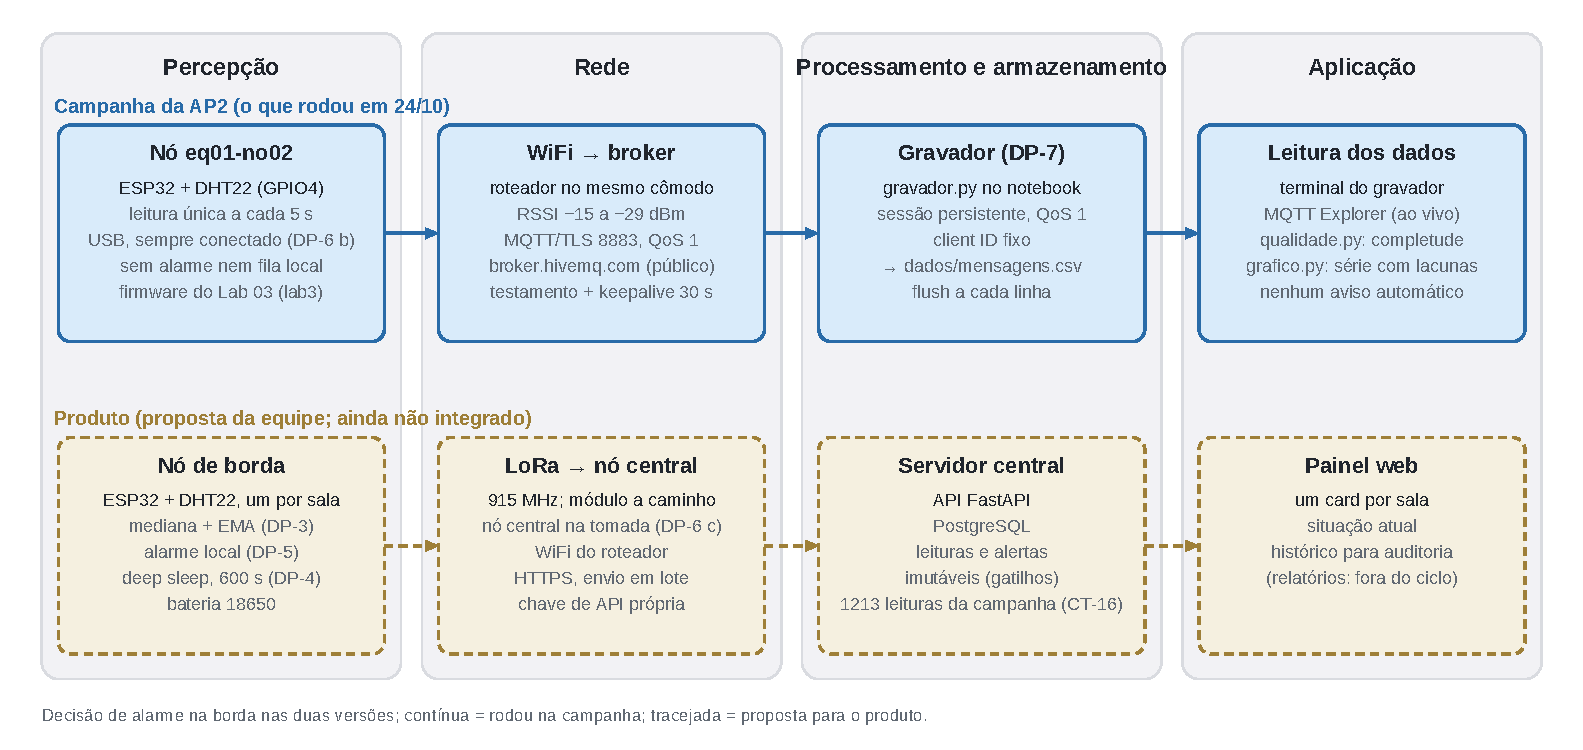
\includegraphics[width=\textwidth]{figuras/arquitetura-ap2.pdf}
\caption{Arquitetura do sistema em camadas: em cima, o que rodou na
  campanha da AP2; embaixo, a arquitetura proposta para o produto}
\label{fig:arquitetura}
\fonte{Elaborada pela equipe.}
\end{figure}

\section{Componentes e decisões de projeto}
\label{sec:componentes}

\begin{orientacao}
Uma caixa por decisão que a equipe realmente tomou. Três a cinco caixas
em um relatório de \rotuloAP\ é a faixa esperada. Candidatas típicas:
escolha do sensor, escolha do atuador, onde fica o limiar de decisão,
como o sistema se comporta sem energia, e por que o dado é (ou não é)
gravado localmente.
\end{orientacao}

\begin{decisao}{Escolha do sensor de temperatura e umidade}
\alternativas{DS18B20 (só temperatura, exigiria um segundo sensor e um
  segundo pino para a umidade), BME280 (mede temperatura, umidade e
  pressão via I\textsuperscript{2}C, custo mais alto) e sensor
  industrial calibrado do tipo usado pelos concorrentes comerciais
  (Novus, Testo), com incerteza de laboratório mas custo por unidade
  de milhares de reais.}
\criterio{O ambiente exige as duas grandezas no mesmo ponto de
  medição (\RF{01}); o custo por sala precisa caber em \RNF{03}
  ($\leq$ R\$\,150,00); o componente precisa estar disponível para a
  equipe.}
\escolha{DHT22 / AM2302.}
\evidencia{O DHT22 mede temperatura e umidade relativa em um único
  chip, por R\$\,39,90 (Tabela~\ref{tab:bom}), contra um DS18B20 que resolveria
  apenas a temperatura e ainda exigiria um sensor de umidade à parte
  --- mais um componente, mais um pino, mais um ponto de falha. A
  incerteza declarada em \folhadedados{} ($\pm$\SI{0.5}{\celsius} e
  $\pm 2$--\SI{5}{\percent} de UR) é suficiente para sinalizar desvio
  de faixa, que é o que \RF{02}/\RF{03} exigem --- o projeto não
  precisa da precisão de um datalogger de laboratório. Com o ESP32
  (R\$\,39,00), o nó completo fica em R\$\,105,20 com protoboard,
  alarme e componentes de reserva (Tabela~\ref{tab:bom}), cerca de
  trinta vezes mais barato que os
  concorrentes comerciais levantados na Cap.~\ref{cap:problema}, que
  usam sensores industriais calibrados justamente para justificar o
  preço.}
\consequencia{O conversor A/D já é do sensor (Aula~06): não existe
  sinal bruto para calibrar, e o erro sistemático de fábrica não é
  corrigível por \emph{software} --- apenas declarado junto de cada
  leitura (Seção~\ref{sec:sinal}). O sensor também impõe um intervalo
  mínimo de \SI{2}{\second} entre leituras, o que limita quantas
  amostras cabem em um ciclo de filtragem (Seção~\ref{sec:sinal}).}
\end{decisao}

\begin{decisao}{Tensão de alimentação do DHT22}
\alternativas{Alimentar em 5\,V com conversor de nível lógico
  bidirecional no fio de dado; alimentar em 5\,V com divisor resistivo
  no fio de dado; alimentar diretamente em 3V3.}
\criterio{O ESP32 não tolera 5\,V em seus pinos GPIO --- a tensão
  máxima admitida fica em torno de \SI{3.6}{\volt} (Aula~03) --- e o
  dano por sobretensão costuma ser silencioso e cumulativo, não
  imediato.}
\escolha{Alimentar o DHT22 em 3V3.}
\evidencia{O DHT22 aceita de 3,3 a 5,5\,V (\folhadedados{}). Alimentado
  em 3V3, o nível alto do seu pino de dado também sai em
  $\approx$\SI{3.3}{\volt}, compatível diretamente com o GPIO do
  ESP32.}
\consequencia{Elimina a necessidade de conversor de nível ou divisor
  resistivo no fio de dado, ao custo de exigir um cabo mais curto até
  o sensor caso a instalação futura precise de mais distância --- se
  isso ocorrer, a alimentação em 5\,V com conversor de nível volta a
  ser a opção recomendada, não o divisor resistivo, que arredonda as
  bordas do sinal em barramentos mais rápidos.}
\end{decisao}

\begin{decisao}{Filtragem da leitura do sensor}
\alternativas{Usar a leitura única do DHT22 sem filtro; aplicar apenas
  uma média aritmética das últimas N leituras; aplicar mediana de N
  amostras por ciclo combinada a uma média exponencial (EMA) entre
  ciclos.}
\criterio{Robustez a uma leitura isolada inválida (falha de
  \emph{timing} ou ruído elétrico no fio de dado, e não ruído de
  sinal analógico, já que o conversor é do próprio sensor --- Aula~06)
  sem herdar o atraso de uma janela longa, dado o custo em tempo
  acordado (e portanto em energia) de cada amostra extra.}
\escolha{Mediana de 5 amostras por ciclo de leitura, seguida de EMA
  entre ciclos de sono ($\alpha = 0{,}30$).}
\evidencia{A mediana descarta com eficiência um valor isolado
  incoerente sem distorcer o resultado inteiro, ao contrário de uma
  média aritmética simples. O custo é declarado: como o próprio
  sensor exige um intervalo mínimo de \SI{2}{\second} entre leituras,
  5 amostras custam cerca de \SI{8,4}{\second} de nó acordado por
  ciclo. Quando menos de 3 das 5 amostras são válidas, o
  \emph{firmware} declara falha em vez de calcular uma mediana pouco
  confiável.}
\consequencia{Cada ciclo de leitura consome mais tempo acordado do que
  uma leitura única resolveria, o que entra diretamente no orçamento
  de energia (Seção~\ref{sec:energia}).}
\end{decisao}

\begin{decisao}{Gerenciamento de energia entre leituras}
\alternativas{\emph{Modem-sleep}, \emph{light-sleep} e \emph{deep
  sleep} (as três estratégias de economia de energia do ESP32
  discutidas na Aula~08).}
\criterio{Autonomia de bateria nos nós de borda, que segundo a
  Cap.~\ref{cap:requisitos} podem ficar em pontos sem tomada
  acessível (dentro de um freezer, por exemplo), onde a troca
  frequente de bateria é indesejável e a fiação até a rede elétrica
  nem sempre é viável.}
\escolha{Deep sleep, com única fonte de despertar por temporizador.}
\evidencia{É o único dos três modos em que quase todo o chip desliga,
  o que dá autonomia de dias a meses em vez de horas --- ao custo de
  que a RAM comum se perde a cada ciclo, e o programa recomeça do
  \texttt{setup()} a cada despertar (Aula~08).}
\consequencia{Todo o \emph{firmware} precisou ser reorganizado para
  caber dentro do \texttt{setup()} (Seção~\ref{sec:firmware}), e as
  poucas variáveis que precisam sobreviver ao sono --- contador de
  despertares, médias exponenciais, contagem de falhas consecutivas
  --- são declaradas em memória RTC (\texttt{RTC\_DATA\_ATTR}), a
  única que atravessa o \emph{deep sleep}.}
\end{decisao}

\begin{decisao}{Onde processar os dados agregados do sistema}
\alternativas{Processamento na borda (o próprio nó ESP32 calcula
  histórico, tendências e regras mais complexas) versus processamento
  em um servidor central, para o qual os nós enviariam apenas as
  leituras.}
\criterio{Custo energético por ciclo em um nó alimentado por bateria
  (Apêndice~\ref{ap:energia}), já que qualquer processamento adicional
  mantém a CPU acordada por mais tempo em vez de voltar ao \emph{deep
  sleep}.}
\escolha{Processamento em servidor central; o nó de borda permanece
  responsável apenas pela leitura, pela filtragem local (mediana +
  média exponencial) e pela decisão simples de alarme dentro da faixa
  configurada.}
\evidencia{O estado de \emph{deep sleep} já responde por cerca de
  68\,\% do consumo diário estimado mesmo sendo o de menor corrente
  instantânea (Apêndice~\ref{ap:energia}); qualquer tempo extra de CPU
  acordada para processamento teria impacto direto e desproporcional
  na autonomia da bateria.}
\consequencia{A arquitetura distribuída (nó~+~servidor central) foi o
  objeto da AP2. O nó continua decidindo só o alarme, mas a decisão
  não evitou retrabalho: o nó da AP1, em \emph{deep sleep}, não foi
  integrado à rede neste ciclo, e unir a leitura filtrada e o alarme
  ao \emph{firmware} de comunicação é a primeira tarefa do próximo
  (\DP{6}, Cap.~\ref{cap:conclusao}).}
\end{decisao}

\subsection*{Decisões do Módulo 2}
\phantomsection
\addcontentsline{toc}{subsection}{Decisões do Módulo 2}

\begin{orientacao}
Novo na AP2. A escolha da tecnologia de comunicação fica na
Seção~\ref{sec:tecnologia}; aqui entram as decisões de
\emph{arquitetura} que mudaram por causa dela. A caixa abaixo registra
o conflito mais evidente entre a AP1 e a AP2: o nó da AP1 dorme em
\emph{deep sleep} (\DP{4}), e o \emph{keepalive} e o testamento do MQTT
pressupõem uma conexão que permanece aberta. Preencham com a decisão
que a equipe tomou de fato.
\end{orientacao}

\begin{decisao}{Deep sleep da AP1 \emph{versus} conexão permanente com o \emph{broker}}
\alternativas{(a) Manter o \emph{deep sleep} da AP1: a cada despertar,
  associar à rede, conectar ao \emph{broker}, publicar e desconectar;
  (b) abandonar o \emph{deep sleep} e manter o nó conectado, em
  \emph{modem-sleep} ou \emph{light-sleep}, com \emph{keepalive} e
  testamento ativos; (c) separar os papéis: o nó de borda mantém o
  \emph{deep sleep} e só liga o rádio para mandar a leitura por LoRa a
  um nó central na tomada, que fica conectado à internet.}
\criterio{Autonomia (\RNF{01}) contra a capacidade de saber que o nó
  caiu (\RF{07}) e de receber configuração pelo tópico \texttt{config};
  custo de associação ao WiFi e de \emph{handshake} TLS a cada
  despertar (Seção~\ref{sec:custo-radio}); disponibilidade de tomada no
  ponto de instalação (Seção~\ref{sec:local}).}
\escolha{No produto, a equipe propõe (c). Na campanha deste ciclo, com um único nó
  falando direto com o roteador, (b): nó alimentado pela USB, sempre
  conectado, com o \emph{firmware} do Lab~03, sem \emph{deep sleep}
  (branch \texttt{lab3}).}
\evidencia{Na bancada (23/10), um ciclo completo de rádio --- associar,
  obter IP, conectar, publicar e desligar --- levou \SI{2,27}{\second} de
  mediana em HTTP e \SI{3,16}{\second} com TLS, com máximo de
  \SI{8,99}{\second}; só o DHCP custa \SI{1,5}{\second}. Pela opção (a),
  o rádio entra com \SI{29,7}{\mAh}/dia (pior ciclo HTTP, \SI{2,48}{\second}),
  o total vai de \SI{69,4}{} para \SI{98,9}{\mAh}/dia (o sono encolhe na mesma
  medida), e a autonomia cai de 30 para 21~dias (Apêndice~\ref{ap:energia}). E
  ainda tira o sentido do testamento: o nó que dorme some do
  \emph{broker} a cada ciclo, e o \texttt{offline} deixa de distinguir um
  nó morto de um nó dormindo. Na opção (c), não há associação nem DHCP:
  um pacote LoRa de 8 bytes fica \SI{57}{\milli\second} no ar em SF7 e
  \SI{1,48}{\second} em SF12 (conta do ar da Aula~14), e o rádio entra
  com cerca de 2 a \SI{3}{\mAh}/dia (\folhadedados, matriz de 22/09),
  o que leva a autonomia a $\approx$29~dias. O número só será medido
  quando o módulo LoRa chegar.}
\consequencia{Na opção (b), a autonomia da AP1 deixa de valer: o nó da
  campanha depende de tomada, e a máquina de estados da
  Seção~\ref{sec:firmware} passa a ser um laço que nunca dorme, com
  \texttt{mqtt.loop()} chamado mais de uma vez a cada \SI{45}{\second}. Na
  opção (c), o testamento passa a ser do nó central; um nó de borda morto
  aparece como sala sem leitura. Esta decisão deixaria de valer se o
  ponto de instalação não tiver tomada e não houver nó central ao
  alcance: aí a opção (a) volta, com a autonomia de cerca de 21~dias.}
\end{decisao}

\begin{decisao}{Quem guarda o dado}
\alternativas{(a) O nó guarda as leituras na \emph{flash} e alguém as
  descarrega depois; (b) o \emph{broker} guarda, com mensagens retidas;
  (c) um assinante guarda: o gravador, com sessão persistente, grava cada
  mensagem em CSV; no produto, o banco do servidor.}
\criterio{Nenhuma leitura pode depender de alguém estar olhando
  (\RNF{08}), e o registro precisa sobreviver a uma auditoria (o motivo
  do produto, Cap.~\ref{cap:problema}).}
\escolha{(c). Na campanha, o gravador do Lab~03 com \emph{client ID}
  fixo, sessão persistente e QoS~1 nas duas pernas. No produto, o banco
  PostgreSQL do servidor, em que leituras e alertas não podem ser
  alterados nem apagados (gatilhos no banco).}
\evidencia{O \emph{broker} só guarda a última mensagem retida de cada
  tópico, e não a série: retida, a telemetria faria um painel recém-aberto
  mostrar uma leitura velha como atual. O gravador grava e dá
  \emph{flush} a cada mensagem, então uma queda do notebook perde no
  máximo a linha em curso; com o gravador parado, o \emph{broker} guarda
  as mensagens da sessão e as entrega na volta (\CT{12}: 6 leituras
  depois de \SI{32}{\second} parado, nos testes de falha, e 100 leituras
  depois de \SI{8,7}{\minute}, no início da campanha, todas com o
  \texttt{ts} original e sem buraco no \texttt{seq}).}
\consequencia{O gravador vira uma peça que alguém precisa manter ligada
  (Tabela~\ref{tab:pecas}), e a sessão persistente só protege enquanto o
  \emph{broker} mantiver a fila. O que o nó mede sem conexão com o
  \emph{broker} não é guardado por ninguém, a menos que o nó tenha fila
  local (\RF{06}). O \emph{firmware} da campanha não tem: na fase
  degradada da campanha, cerca de 740 leituras deixaram de existir
  (Seção~\ref{sec:qualidade}).}
\end{decisao}

\section{Mapa de barramento}
\label{sec:barramento}

\begin{orientacao}
Resuma aqui, em um parágrafo, o que o mapa de barramento entregue em
01/09 decidiu: quantos dispositivos, em quais barramentos, e qual foi o
conflito mais difícil de resolver. A tabela completa vai no
Apêndice~\ref{ap:barramento}, já formatada. Se a equipe mudou de
componente depois da Aula 06, atualize o apêndice --- mapa
desatualizado no relatório é a forma mais barata de perder pontos em
documentação.
\end{orientacao}

O mapa completo está no Apêndice~\ref{ap:barramento}.

O nó usa, além da alimentação, o dado do DHT22 (protocolo
proprietário de um fio, ponto a ponto, análogo em espírito ao 1-Wire
visto na Aula~06 mas não compatível com ele), duas saídas de alarme
(buzzer e LED), um LED de status digital para diagnóstico em bancada
e a leitura opcional de tensão de bateria por um divisor resistivo no
ADC1, o conversor que continua confiável com o WiFi ligado. O conflito mais relevante
resolvido nesta etapa não foi de pino ocupado, e sim de \emph{classe}
de pino: o dado do DHT22 precisa também escrever, o que descarta de
saída os pinos \texttt{A2}--\texttt{A5} (só entrada) como candidatos,
além dos pinos de \emph{strapping} de boot (\texttt{GPIO2},
\texttt{GPIO12}) listados entre as armadilhas da Aula~03.

\section{Orçamento de energia}
\label{sec:energia}

\begin{orientacao}
Mesmo padrão: um parágrafo com o total diário, a fonte de alimentação
escolhida e a autonomia estimada; a tabela completa no
Apêndice~\ref{ap:energia}. Diga qual estado domina o consumo. Esse
número costuma ser a decisão de projeto mais importante do ciclo, e
quase nunca é de \emph{firmware}.
\end{orientacao}

O orçamento completo está no Apêndice~\ref{ap:energia}.

Com a leitura a cada \RF{01} (10 min) e os valores de corrente
declarados no \emph{firmware} (\SI{45}{\milli\ampere} do ESP32 acordado
mais \SI{1,5}{\milli\ampere} do DHT22 em leitura, \folhadedados; \SI{2}{\milli\ampere} em deep sleep, \bancada), o
consumo diário estimado do nó de sensoriamento fica em torno de
\SI{69}{\mAh}/dia. Quem domina esse total não é o DHT22 --- que entra
com menos de \SI{0.02}{\mAh} por ciclo --- e sim os \SI{588}{\second}
de deep sleep entre cada leitura, o que confirma a expectativa da
Aula~08 de que a corrente de repouso da placa, não o sensor, é quem
dimensiona o sistema. Este número \textbf{não inclui} o consumo do
alarme (buzzer/LED): o alarme já está no \emph{firmware} da AP1
(Seção~\ref{sec:decisao}), mas a corrente dele é uma \estimativa{} de
\SI{35}{\milli\ampere} e só ocorre enquanto a leitura está fora da faixa,
o que não cabe numa conta por ciclo; ela precisa ser medida em bancada
antes de fechar o orçamento final. Com uma bateria 18650 de \SI{2600}{\mAh} e
80\,\% de profundidade de descarga útil, a autonomia estimada
\emph{apenas do sensoriamento} seria de cerca de 30 dias --- um piso,
não o número final do projeto.

Na AP2 entra a linha que faltava: o rádio. Com o tempo de rádio medido
na Seção~\ref{sec:custo-radio} (o pior de 10 ciclos HTTP,
\SI{2,48}{\second}) e a corrente do medidor USB
(\SI{300}{\milli\ampere}), o nó que acorda, publica e volta a dormir a
cada \SI{10}{\minute} passa a consumir \SI{98,9}{\mAh}/dia, e a
autonomia estimada cai de 30 para \textbf{21 dias}. O estado que
dimensiona o sistema continua sendo o \emph{deep sleep}, mas agora com
47\,\% do consumo, e o rádio já responde por 30\,\%. Com TLS, como no
MQTT da campanha, o ciclo de rádio fica 1,39 vez mais longo na mediana
(\SI{3,16}{\second}); com essa duração, o consumo sobe para cerca de
\SI{107}{\mAh}/dia (19 dias). Esses números
valem para o nó a bateria; o nó da campanha ficou ligado à USB, sempre
conectado (\DP{6}), e a corrente dele não foi medida.

\section{Lista de materiais}
\label{sec:bom}

\begin{table}[H]
\centering
\caption{Lista de materiais do protótipo}
\label{tab:bom}
\footnotesize
\begin{tabular}{@{}L{5.2cm}C{1.6cm}R{2.4cm}R{2.6cm}L{2.0cm}@{}}
\toprule
\textbf{Item} & \textbf{Qtd.} & \textbf{Unitário (R\$)} & \textbf{Total (R\$)} & \textbf{Origem} \\
\midrule
Placa ESP32 WROOM (D1 R32) & 1 & 39,00 & 39,00 & compra \\
Sensor DHT22 / AM2302      & 1 & 39,90 & 39,90 & compra \\
Resistor 10\,k$\Omega$ (pull-up do dado) & 1 & 0,50 & 0,50 & compra \\
Resistores 100\,k$\Omega$ (divisor de \texttt{VBAT}, opcional) & 2 & 0,50 & 1,00 & compra \\
LED de status & 1 & 0,50 & 0,50 & compra \\
Buzzer ativo (alarme sonoro) & 1 & 5,00 & 5,00 & compra \\
LED infravermelho 3\,mm (reserva de estoque para módulo futuro) & 1 & 2,00 & 2,00 & compra \\
Receptor infravermelho TL1838/TI1838 (reserva de estoque para módulo futuro) & 1 & 1,90 & 1,90 & compra \\
Transistor BC548 (reserva de estoque para módulo futuro) & 2 & 0,20 & 0,40 & compra \\
Protoboard e jumpers & 1 & 15,00 & 15,00 & compra \\
\midrule
\multicolumn{3}{@{}r}{\textbf{Total do protótipo montado}} & \textbf{105,20} & \\
\midrule
Módulo LoRa (\SI{915}{\mega\hertz}; encomendado, não chegou a tempo) & 1 & 40,00 a 60,00 & 40,00 a 60,00 & \estimativa \\
\multicolumn{3}{@{}r}{\textbf{Total com o módulo LoRa}} & \textbf{145,20 a 165,20} & \\
\bottomrule
\end{tabular}
\fonte{Elaborada pela equipe, com base nos preços de referência do README do firmware. O preço do módulo LoRa é a faixa da matriz de 22/09 (RFM95/SX1276), e não o valor pago.}
\end{table}

Mesmo com o buzzer já orçado, o protótipo montado (R\$\,105,20) cabe
com folga no teto de \RNF{03} (R\$\,150,00 por sala). A folga some com
o rádio do produto: o módulo LoRa (\DP{8}) custa de R\$\,40 a 60, e o
ponto passa a R\$\,145,20 a 165,20. Sem os itens de reserva de estoque
(R\$\,4,30), que não fazem parte do nó, fica em R\$\,140,90 a 160,90:
no limite do teto, ou acima dele. O \RNF{03} está atendido pelo nó que
existe hoje, e precisa ser conferido com o preço real do módulo quando
ele chegar; a protoboard e os \emph{jumpers} (R\$\,15,00), que uma placa
definitiva substituiria, são a primeira folga a buscar. Mesmo no pior
caso, o custo por ponto continua cerca de vinte vezes menor que o dos
concorrentes comerciais da Cap.~\ref{cap:problema}.

% =====================================================================
%  Capítulo 4 — Implementação
% =====================================================================
\chapter{Implementação}
\label{cap:implementacao}
\rubricaFuncionalidade

\begin{orientacao}
Este é o capítulo que responde \enquote{o protótipo funciona?}, que vale
30\,\% da nota. Ele descreve o que foi construído, com detalhe
suficiente para que outra equipe consiga reproduzir. O critério prático:
se alguém com o repositório e este capítulo na mão não conseguir montar
e rodar o sistema, falta coisa aqui.
\end{orientacao}

Este capítulo descreve \textbf{dois \emph{firmwares}}. O primeiro é o
nó da AP1, \texttt{esp32\_dht22.ino}, que lê, filtra e alarma, mas não
publica. Em relação à primeira versão dele, três coisas mudaram e são
detalhadas aqui: o intervalo entre
leituras e os limiares de faixa deixaram de ser constantes de
compilação e passaram a ser \textbf{parâmetros gravados em memória
não-volátil} (biblioteca \texttt{Preferences}); o \textbf{alarme local}
(buzzer ativo + LED) foi integrado ao \emph{firmware}; e, enquanto a
leitura está fora da faixa, o nó passa a acordar em um
\textbf{intervalo mais curto} do que o de rotina. O custo de cada uma
dessas mudanças em tempo acordado e em energia é declarado nas seções
correspondentes.

O segundo é o \emph{firmware} de comunicação, construído na AP2 à
parte, sobre o nó MQTT do Lab~03 (Seção~\ref{sec:firmware-com}, branch
\texttt{lab3}): o nó entra no WiFi, acerta o relógio por NTP, conecta ao
\emph{broker} por TLS deixando um testamento \texttt{offline}, publica
\texttt{online} retido, assina o próprio tópico de configuração e
publica cada leitura no contrato de dados da
Seção~\ref{sec:contrato-dados}, com QoS~1. Em relação ao sketch-base, a
equipe trocou o sensor do exemplo (um MPU6050 em I\textsuperscript{2}C)
pelo DHT22 no \texttt{GPIO4}, o mesmo pino da AP1, com a biblioteca
DHTesp; definiu a equipe e o nó (\texttt{eq01}, \texttt{no02}); e
passou o monitor serial de 9600 para \SI{115200}{\baud}, a velocidade que
o roteiro do Lab~03 manda usar.
\textbf{Esse \emph{firmware} não tem} a leitura filtrada da AP1 (mediana
de 5 amostras e EMA), o alarme local, a configuração na NVS, o
\emph{deep sleep}, o \texttt{boot} nem fila local: foi ele que rodou na
campanha, alimentado pela USB (\DP{6}). As seções de montagem, filtragem
e decisão de alarme abaixo descrevem o nó da AP1 (\texttt{esp32\_dht22.ino}),
que não rodou na campanha; unir as duas versões fica para o próximo
ciclo (Cap.~\ref{cap:conclusao}). No fim da Seção~\ref{sec:firmware-com},
dois \emph{firmwares} de bancada completam o quadro: o ciclo HTTP de um
nó que dorme entre leituras (Seção~\ref{sec:firmware-http}) e o enlace
ESP-NOW e BLE entre um nó de borda e um nó central, montado no lugar do
LoRa enquanto o módulo não chegava (Seção~\ref{sec:espnow-bancada}), os
dois com o DHT22 no mesmo \texttt{GPIO4}.

\section{Montagem}
\label{sec:montagem}

\begin{orientacao}
Esquemático (ou foto anotada da montagem) mais uma tabela de ligações.
Aponte explicitamente onde há divisor de tensão, resistor de
\emph{pull-up}, transistor ou diodo de roda livre, e por quê. Módulo de
\SI{5}{\volt} ligado direto no ESP32 é a armadilha clássica: se o
projeto tem algum, mostre aqui como foi resolvido.
\end{orientacao}

O protótipo é montado em protoboard sobre a placa ESP32 D1 R32. Além
da alimentação, há quatro sinais: o dado do DHT22, o buzzer, o LED de
alarme e o LED de status de bancada; a leitura de tensão de bateria é
opcional e só existe quando o nó é alimentado por bateria. A
Tabela~\ref{tab:ligacoes} resume as ligações.

\begin{table}[H]
\centering
\caption{Ligações do protótipo na placa ESP32 D1 R32}
\label{tab:ligacoes}
\footnotesize
\begin{tabular}{@{}L{3.6cm}L{3.2cm}L{6.6cm}@{}}
\toprule
\textbf{Componente} & \textbf{Pino (GPIO / rótulo)} & \textbf{Observação} \\
\midrule
DHT22 --- VCC  & 3V3 & alimentado em 3V3, não em 5\,V (\DP{2}) \\
DHT22 --- GND  & GND & terra comum com a placa \\
DHT22 --- DATA & GPIO4 (A1) & \emph{pull-up} de \SI{10}{\kilo\ohm} até o 3V3 \\
Buzzer ativo (+) & GPIO26 (D4) & acionado em nível alto \\
Buzzer ativo ($-$) & GND & \\
LED de alarme (ânodo) & GPIO27 (D5) & resistor limitador de $\approx$\SI{330}{\ohm} em série \\
LED de status (ânodo) & GPIO25 (D3) & resistor limitador; só para bancada \\
Divisor de \texttt{VBAT} (opcional) & GPIO34 (A2) & \SI{100}{\kilo\ohm}/\SI{100}{\kilo\ohm} entre o + da bateria e o GND; ADC1, só entrada \\
\bottomrule
\end{tabular}
\fonte{Elaborada pela equipe, com base no README do firmware.}
\end{table}

Quatro pontos da montagem merecem registro explícito:

\begin{enumerate}[label=\alph*)]
  \item \textbf{Não há divisor de tensão nem conversor de nível no fio
    de dado.} Como o DHT22 é alimentado em 3V3 (\DP{2}), o nível alto
    do seu pino de dado já sai em $\approx$\SI{3.3}{\volt}, compatível
    com o GPIO do ESP32. O único divisor do circuito é o de
    \texttt{VBAT}, que serve a outra finalidade (item~d).
  \item \textbf{O \emph{pull-up} de \SI{10}{\kilo\ohm} é parte do
    circuito, não acessório.} O barramento do DHT22 é de dreno aberto;
    sem o resistor, a leitura devolve \texttt{NaN} em todas as
    amostras. Muitos módulos DHT22 já trazem esse resistor na placa;
    nesse caso não se adiciona outro, o que só empobreceria o sinal.
  \item \textbf{Buzzer e LED de alarme são acionados diretamente pelo
    GPIO.} A escolha é aceitável para um buzzer ativo de 3V3 de baixa
    corrente e um LED com resistor limitador, mas depende de um número
    que ainda não foi medido: a corrente somada dos dois é hoje uma
    \estimativa{} de \SI{35}{\milli\ampere}
    (Apêndice~\ref{ap:energia}). Se a medição em bancada confirmar um
    valor acima do que o pino entrega com segurança (a Aula~03 indica
    cerca de \SI{12}{\milli\ampere} por GPIO como referência
    conservadora), o buzzer passa a ser chaveado por um transistor NPN
    com resistor de base, com o coletor no ramo de alimentação e não
    no pino. O \emph{firmware} não muda nesse caso: o pino continua
    escrevendo \texttt{HIGH}/\texttt{LOW}.
  \item \textbf{O divisor de \texttt{VBAT} reduz a tensão da bateria à
    metade} ($V_{\text{out}} = V_{\text{in}} \cdot R_2/(R_1+R_2)$, com
    $R_1 = R_2 = \SI{100}{\kilo\ohm}$), de modo que uma célula Li-ion a
    \SI{4.2}{\volt} chega ao ADC como \SI{2.1}{\volt}, dentro da faixa
    útil de $\approx$\SI{3.1}{\volt} da atenuação padrão. O GPIO34 foi
    escolhido por pertencer ao ADC1, que continua confiável com o rádio
    ligado --- decisão tomada na AP1 e que passou a importar neste
    ciclo, com o rádio em uso.
\end{enumerate}

\begin{figure}[H]
\centering
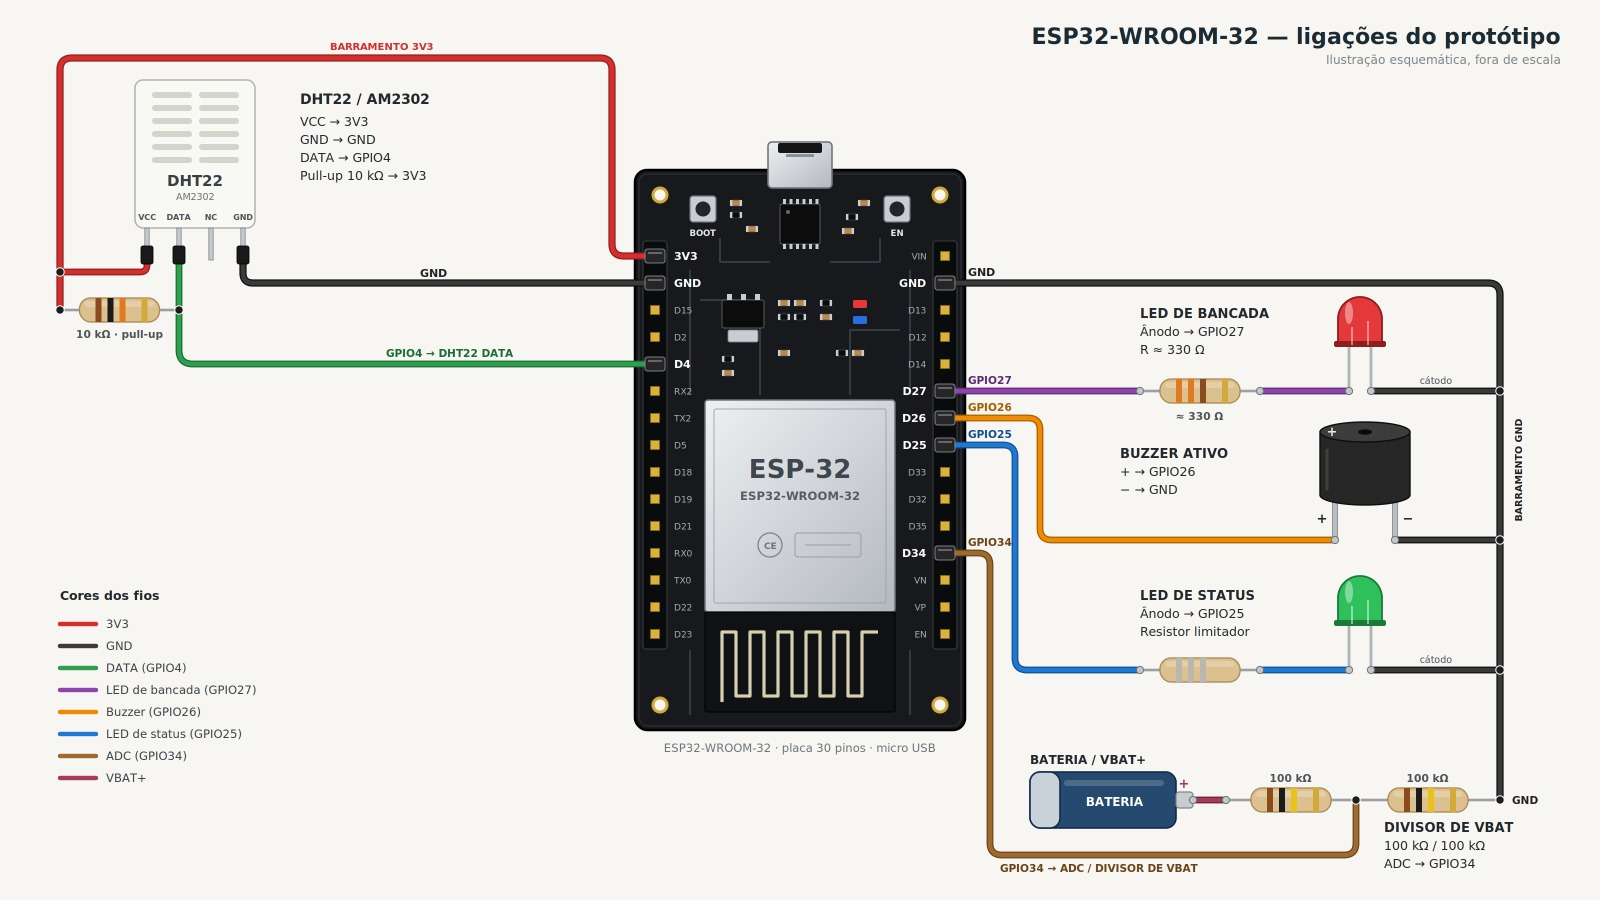
\includegraphics[width=0.9\textwidth]{figuras/mapa-de-barramento.jpeg}
\caption{Ligações do protótipo na placa ESP32}
\label{fig:montagem}
\fonte{Elaborada pela equipe.}
\end{figure}

\section{Estrutura do firmware}
\label{sec:firmware}

\begin{orientacao}
Descreva a máquina de estados do sistema: quais estados existem, o que
dispara cada transição e quanto tempo o sistema passa em cada um. Os
estados daqui têm de ser os mesmos do orçamento de energia
(Apêndice~\ref{ap:energia}) --- se não forem, um dos dois está errado.

Inclua trechos de código apenas quando o trecho \emph{decide} alguma
coisa: o laço de temporização, a histerese, o tratamento de falha de
leitura. Código de inicialização de biblioteca não precisa aparecer;
ele está no repositório.
\end{orientacao}

Como o nó usa \emph{deep sleep} entre leituras (\DP{4}), o
\texttt{loop()} nunca é retomado: a cada despertar o programa recomeça
do \texttt{setup()}, e é dentro dele que mora todo o ciclo. O sistema
tem quatro estados, os mesmos do Apêndice~\ref{ap:energia}:

\begin{description}[style=unboxed, leftmargin=0.6cm]
  \item[\textsc{acorda e configura}] --- inicializa os pinos com buzzer
    e LED de alarme em \texttt{LOW}, carrega a configuração da NVS e
    abre uma janela de \SI{4}{\second} para comandos pela porta serial
    (Seção~\ref{sec:config}). Se nada chegar, segue adiante. Dura
    $\approx$\SI{4}{\second}.
  \item[\textsc{lê}] --- faz 5 amostras do DHT22 espaçadas de
    \SI{2.1}{\second}, calcula a mediana e atualiza a média exponencial
    (Seção~\ref{sec:sinal}). Dura $\approx$\SI{8,4}{\second}.
  \item[\textsc{aciona o atuador}] --- só existe no ciclo em que a
    leitura está fora da faixa: buzzer e LED ficam ligados por
    \SI{3}{\second} e são desligados antes do sono
    (Seção~\ref{sec:decisao}). Nos demais ciclos dura zero.
  \item[\textsc{dorme}] --- \emph{deep sleep} com despertar por
    temporizador. A duração depende do resultado do ciclo:
    \SI{600}{\second} (intervalo normal, \RF{01}) se a leitura estava
    dentro da faixa, ou \SI{60}{\second} (intervalo de alarme) se
    estava fora. Ambos são configuráveis (Seção~\ref{sec:config}).
\end{description}

As transições são todas sequenciais e temporizadas, exceto a que decide
qual intervalo de sono usar, que depende da avaliação de faixa. Os
$\approx$\SI{12}{\second} somados dos três estados acordados são o
\texttt{T\_ACORDADO\_S} do orçamento de energia (\bancada). A
Listagem~\ref{lst:laco} mostra o esqueleto do \texttt{setup()} com as
decisões que importam; a inicialização de bibliotecas e as mensagens de
diagnóstico ficaram no repositório.

\begin{lstlisting}[style=arduino,
  caption={Esqueleto do ciclo: tudo mora no \texttt{setup()}, e o intervalo de sono é decidido no fim},
  label={lst:laco}]
RTC_DATA_ATTR float    emaTemp = NAN, emaHum = NAN;   // atravessam o sono
RTC_DATA_ATTR uint32_t falhasConsecutivas = 0;

void setup() {
  digitalWrite(BUZZER_PIN, LOW);      // estado seguro antes de tudo
  digitalWrite(ALARME_LED_PIN, LOW);
  carregarConfiguracao();             // NVS -> cfg (intervalos e faixa)
  talvezEntrarModoConfig();           // janela de 4 s por comandos SET

  float t, h;
  bool emAlarme = false;
  if (lerDHTFiltrado(t, h)) {         // mediana de 5 amostras
    falhasConsecutivas = 0;
    emaTemp = EMA_ALPHA * t + (1.0f - EMA_ALPHA) * emaTemp;
    emaHum  = EMA_ALPHA * h + (1.0f - EMA_ALPHA) * emaHum;
    emAlarme = avaliarAlarme(t, h);   // usa a mediana, nao a EMA
  } else {
    falhasConsecutivas++;             // declara falha; nao inventa numero
  }

  dormir(emAlarme ? cfg.intervaloAlarmeS : cfg.intervaloNormalS);
}

void loop() { /* nunca executa: deep sleep reinicia no setup() */ }
\end{lstlisting}

O que precisa atravessar o sono está em memória RTC
(\texttt{RTC\_DATA\_ATTR}): contador de despertares, as duas médias
exponenciais e a contagem de falhas consecutivas. Tudo o mais é
recalculado a cada ciclo. A configuração, por sua vez, sobrevive de
outra forma --- pela NVS, que persiste mesmo com o nó desligado.

\subsection{Configuração em tempo de execução}
\label{sec:config}

Na primeira versão, o intervalo de leitura era um \texttt{\#define}.
Isso atende um único cenário, mas a Cap.~\ref{cap:requisitos} exige
que a faixa seja configurável por ambiente (\RF{02}), e o mesmo
argumento vale para o intervalo: uma câmara fria de farmácia e uma sala
de equipamentos não pedem a mesma frequência de checagem, e recompilar
o \emph{firmware} para cada instalação não é solução de produto. Os
seis parâmetros da Tabela~\ref{tab:config} passaram a ser gravados na
NVS pela biblioteca \texttt{Preferences} (inclusa no \emph{core} do
ESP32), sob o \emph{namespace} \texttt{termolog}.

\begin{table}[H]
\centering
\caption{Parâmetros gravados na NVS e seus padrões de fábrica}
\label{tab:config}
\footnotesize
\begin{tabular}{@{}L{4.4cm}L{4.6cm}L{4.4cm}@{}}
\toprule
\textbf{Parâmetro} & \textbf{Comando serial} & \textbf{Padrão de fábrica} \\
\midrule
Intervalo normal entre leituras & \texttt{SET INTERVALO=<s>} & \SI{600}{\second} (\RF{01}) \\
Intervalo enquanto em alarme    & \texttt{SET INTERVALO\_ALARME=<s>} & \SI{60}{\second} \\
Temperatura mínima              & \texttt{SET TEMP\_MIN=<\textdegree C>} & \SI{15}{\celsius} \\
Temperatura máxima              & \texttt{SET TEMP\_MAX=<\textdegree C>} & \SI{25}{\celsius} \\
Umidade relativa mínima         & \texttt{SET UMID\_MIN=<\%>} & 40\,\% UR \\
Umidade relativa máxima         & \texttt{SET UMID\_MAX=<\%>} & 70\,\% UR \\
\bottomrule
\end{tabular}
\fonte{Elaborada pela equipe. Os limiares padrão são os do cenário de validação (farmácia de manipulação, Cap.~\ref{cap:problema}) e devem ser ajustados por ambiente na instalação.}
\end{table}

Os comandos são aceitos pelo monitor serial (\SI{115200}{\baud}) nos
primeiros \SI{4}{\second} após energizar; cada comando aceito é gravado
imediatamente e renova a janela por mais \SI{4}{\second}.
\texttt{SHOW} imprime a configuração em uso e \texttt{RESET} restaura
os padrões. Em campo, sem ninguém na porta serial, a janela expira e o
ciclo segue sozinho com a última configuração gravada.

Duas ressalvas de custo, ambas declaradas para não serem descobertas
depois:

\begin{itemize}
  \item \textbf{O custo da biblioteca em si é desprezível.} A leitura
    da NVS no despertar (\texttt{begin}, seis \texttt{get},
    \texttt{end}) leva alguns milissegundos, invisíveis diante dos
    \SI{8.4}{\second} que o próprio sensor impõe. Escrita só ocorre em
    \texttt{SET}, \texttt{RESET} ou no primeiro boot --- nunca a cada
    ciclo ---, então o desgaste da \emph{flash} não entra na conta.
  \item \textbf{O custo real é a janela serial}, não a biblioteca:
    \SI{4}{\second} de nó acordado a $\approx$\SI{45}{\milli\ampere}
    equivalem a $\approx$\SI{0.05}{\mAh} por ciclo, ou
    $\approx$\SI{7}{\mAh}/dia no intervalo de 10 min --- cerca de
    10\,\% do orçamento diário. Esse tempo já está incluído nos
    \SI{12}{\second} de \texttt{T\_ACORDADO\_S} do
    Apêndice~\ref{ap:energia}; reduzir ou condicionar a janela (por
    exemplo, só abri-la quando a porta serial estiver conectada) é uma
    otimização registrada para o próximo ciclo.
\end{itemize}

Gravar parâmetros na NVS não contradiz a decisão de não guardar
leituras no nó (\DP{7}): o que se guarda é meia
dúzia de números fixos até que alguém os troque, não uma série
temporal.

\section{Lógica de decisão e atuação}
\label{sec:decisao}

\begin{orientacao}
Qual é a regra que liga a leitura ao atuador, e por que ela tem essa
forma. Se há histerese, diga quais são os dois limiares e como foram
escolhidos --- limiar escolhido \enquote{no olho} é resposta aceitável
desde que declarada e acompanhada do que aconteceu quando a equipe
testou. Se não há histerese, explique por que o relé não castanhola.
\end{orientacao}

A regra é uma comparação de faixa sobre a mediana do ciclo: o alarme
dispara se a temperatura estiver abaixo do mínimo ou acima do máximo,
\emph{ou} se a umidade estiver abaixo do mínimo ou acima do máximo
(\RF{02}/\RF{03}). A comparação usa a mediana das 5 amostras, e não a
média exponencial, de propósito: a EMA suaviza justamente o tipo de
desvio que o alarme existe para pegar, e um alarme que reage com atraso
a uma câmara fria aquecendo não cumpre \RNF{02}. A
Listagem~\ref{lst:alarme} mostra a função inteira.

\begin{lstlisting}[style=arduino,
  caption={Avaliação de faixa e acionamento do alarme local (buzzer + LED)},
  label={lst:alarme}]
bool avaliarAlarme(float temperaturaC, float umidadeRH) {
  bool foraDaFaixa = (temperaturaC < cfg.tempMinC) ||
                     (temperaturaC > cfg.tempMaxC) ||
                     (umidadeRH   < cfg.umidMinPct) ||
                     (umidadeRH   > cfg.umidMaxPct);
  if (foraDaFaixa) {
    digitalWrite(BUZZER_PIN, HIGH);     // buzzer ativo: nivel alto = som
    digitalWrite(ALARME_LED_PIN, HIGH);
    delay(ALARME_DURACAO_MS);           // 3 s
    digitalWrite(BUZZER_PIN, LOW);
    digitalWrite(ALARME_LED_PIN, LOW);
    return true;                        // -> dormir no intervalo de alarme
  }
  return false;                         // -> dormir no intervalo normal
}
\end{lstlisting}

O acionamento é um \textbf{pulso de \SI{3}{\second} por ciclo}, não um
som contínuo: o buzzer ativo já oscila sozinho e basta manter o pino em
nível alto, mas manter um GPIO ligado durante o \emph{deep sleep}
exigiria \texttt{gpio\_hold\_en()} sobre um pino RTC, o que esta
revisão não faz. Para que um pulso curto não passe despercebido, o nó
compensa \textbf{acordando mais vezes}: enquanto a última leitura
estiver fora da faixa, o próximo sono dura o intervalo de alarme
(\SI{60}{\second}) em vez do normal (\SI{600}{\second}), e o alarme
volta a soar a cada minuto até a condição ser corrigida. Assim que uma
leitura cai dentro da faixa, o pulso simplesmente não ocorre e o nó
volta ao intervalo normal por conta própria --- é isso que atende
\RF{04}, e em até \SI{1}{\minute} após o retorno, bem dentro do limite
de um ciclo exigido.

\begin{table}[H]
\centering
\caption{Parâmetros da lógica de decisão}
\label{tab:limiares}
\footnotesize
\begin{tabular}{@{}L{4.0cm}C{2.6cm}L{6.8cm}@{}}
\toprule
\textbf{Parâmetro} & \textbf{Valor} & \textbf{Como foi escolhido} \\
\midrule
Faixa de temperatura (liga fora dela) & 15 a \SI{25}{\celsius} & cenário de validação (farmácia); configurável por ambiente \\
Faixa de umidade (liga fora dela) & 40 a 70\,\% UR & idem \\
Histerese entre liga e desliga & nenhuma & ver texto: o atuador não tem estado a castanholar \\
Duração do pulso de alarme & \SI{3}{\second} & \estimativa{} (audível em sala; a ajustar após ensaio) \\
Tempo mínimo entre acionamentos & \SI{60}{\second} & intervalo de alarme; \estimativa{} de compromisso energia/resposta \\
\bottomrule
\end{tabular}
\fonte{Elaborada pela equipe.}
\end{table}

\textbf{Por que não há histerese, e por que isso não castanhola.} Um
relé castanhola quando o sinal oscila em torno de um único limiar e o
atuador tem dois estados persistentes que trocam a cada oscilação.
Aqui o atuador não tem estado persistente: ele é ligado e desligado
dentro do mesmo ciclo, e entre dois ciclos há pelo menos
\SI{60}{\second} de sono. O pior caso de uma leitura oscilando na borda
da faixa é, portanto, um pulso de \SI{3}{\second} a cada minuto ---
exatamente o comportamento de alarme desejado, e não um defeito. A
mediana de 5 amostras também reduz a chance de um único valor de borda
disparar o pulso. Se o ensaio \CT{03} mostrar que a borda incomoda na
prática, a histerese entra como um sétimo parâmetro da NVS sem mudar a
estrutura.

\textbf{Custo declarado da mudança de frequência.} Acordar a cada
minuto custa mais que a cada dez. No pior caso --- nó preso fora da
faixa o dia inteiro --- cada ciclo dura \SI{75}{\second}
(\SI{12}{\second} acordado a \SI{46,5}{\milli\ampere}, \SI{3}{\second} de
alarme com mais \SI{35}{\milli\ampere} e \SI{60}{\second} dormindo a
\SI{2}{\milli\ampere}) e consome $\approx$\SI{0,26}{\mAh}; com
\num{1152} ciclos por dia, são $\approx$\SI{295}{\mAh}/dia, contra os \SI{69}{\mAh}/dia
do regime normal. Com a 18650 de \SI{2600}{\mAh} do
Apêndice~\ref{ap:energia}, a autonomia cai de $\approx$30 para
$\approx$7 dias \emph{enquanto o alarme persistir}. A equipe aceita
esse custo porque, por definição, ele só ocorre enquanto algo está
errado --- e sete dias de alarme sem ninguém agir é um problema
operacional, não de bateria. O número usa a corrente de alarme ainda
\estimativa{}; será revisto após a medição em bancada.

\section{Tratamento do sinal}
\label{sec:sinal}

\begin{orientacao}
O que foi feito entre o valor bruto do ADC e o número usado na decisão:
calibração (com a curva e o procedimento), média móvel, descarte de
\emph{outliers}, saturação. Traga o antes e o depois --- um gráfico com
o sinal cru e o sinal tratado vale mais que dois parágrafos. Reaproveite
a análise de ruído de 26/08.
\end{orientacao}

\subsection{Formato de captação do DHT22}

O DHT22 inverte o problema tratado na Aula~05: não há ADC da equipe nem
contagem bruta. O sensor traz o conversor embutido e entrega, por um
protocolo proprietário de um fio, dois números já calibrados de
fábrica --- temperatura em \si{\celsius} com resolução de
\SI{0.1}{\celsius} e umidade relativa em \% UR com resolução de
0,1\,\% --- protegidos por um \emph{checksum} de um byte. A biblioteca
\texttt{DHT} (Adafruit) decodifica o quadro de 40 bits e devolve
\texttt{NaN} quando o \emph{checksum} falha ou o \emph{timing} da
resposta sai da tolerância. Duas consequências fixam o formato de
captação:

\begin{itemize}
  \item \textbf{o erro sistemático não é corrigível por software}: a
    incerteza declarada em \folhadedados{} ($\pm$\SI{0.5}{\celsius};
    $\pm 2$\,\% UR, chegando a $\pm 5$\,\% nas extremidades) é
    impressa junto de cada leitura, para não se perder entre o sensor
    e quem consome o dado (\RNF{04});
  \item \textbf{o sensor impõe um intervalo mínimo de \SI{2}{\second}
    entre leituras}; o \emph{firmware} usa \SI{2.1}{\second}, o que
    limita a 5 o número de amostras que cabem em um ciclo sem
    estourar o tempo acordado orçado.
\end{itemize}

O ruído que resta é de \emph{comunicação}, não de sinal: um bit mal
decodificado por interferência no fio ou por variação de \emph{timing}
produz \texttt{NaN} ou, mais raramente, um valor absurdo isolado --- e
é este o caso de \RNF{05}, quando o compressor da câmara fria liga. A
captação, portanto, é feita em dois estágios com preço declarado:

\begin{enumerate}
  \item \textbf{Mediana de 5 amostras por ciclo.} Cada amostra é uma
    leitura de temperatura e uma de umidade; amostras \texttt{NaN} são
    descartadas na hora. Se menos de 3 das 5 forem válidas, o ciclo é
    declarado como \textbf{falha} --- sem inventar uma mediana a
    partir de dois pontos (Listagem~\ref{lst:leitura}). A mediana
    descarta um \emph{outlier} isolado sem arrastar o resultado, como
    faria uma média aritmética. Custo: $\approx$\SI{8.4}{\second} de
    nó acordado por ciclo.
  \item \textbf{Média exponencial (EMA) entre ciclos}, com
    $\alpha = 0{,}30$, guardada em memória RTC:
    $\text{ema}_{n} = \alpha\,x_n + (1-\alpha)\,\text{ema}_{n-1}$.
    Suaviza a variação natural entre um despertar e o seguinte sem
    exigir histórico nem herdar o atraso de uma janela longa. Custo:
    dois \texttt{float} em RTC; latência de $\approx$3 ciclos para
    acompanhar um degrau. Por isso a EMA é apenas o valor
    \emph{reportado}, e nunca o valor usado na decisão de alarme
    (Seção~\ref{sec:decisao}).
\end{enumerate}

\begin{lstlisting}[style=arduino,
  caption={Captação do DHT22: 5 amostras, descarte de \texttt{NaN}, maioria obrigatória, mediana},
  label={lst:leitura}]
bool lerDHTFiltrado(float &temperaturaC, float &umidadeRH) {
  float amostrasTemp[N_AMOSTRAS], amostrasHum[N_AMOSTRAS];
  int validas = 0;
  for (int i = 0; i < N_AMOSTRAS; i++) {
    float t = dht.readTemperature();
    float h = dht.readHumidity();
    if (!isnan(t) && !isnan(h)) {     // checksum ou timing ruim -> NaN
      amostrasTemp[validas] = t;
      amostrasHum[validas]  = h;
      validas++;
    }
    if (i < N_AMOSTRAS - 1) delay(DHT_MIN_INTERVAL_MS);  // 2100 ms
  }
  if (validas < (N_AMOSTRAS / 2 + 1)) return false;      // < 3 de 5
  temperaturaC = mediana(amostrasTemp, validas);
  umidadeRH    = mediana(amostrasHum, validas);
  return true;
}
\end{lstlisting}

No nó da AP1, o dado sai apenas pela porta serial, no formato da
Listagem~\ref{lst:serial}: mediana e EMA lado a lado, seguidas da
incerteza declarada e, quando há bateria, da tensão lida. O
\emph{firmware} de comunicação da campanha publica, em vez disso, a
leitura única no contrato da Seção~\ref{sec:contrato-dados}; publicar a
mediana é parte da união das duas versões.

\begin{lstlisting}[style=terminal,
  caption={Saída serial de um ciclo com leitura válida},
  label={lst:serial}]
---- Leitura ----
Temperatura (mediana da amostra): 23.40 C
Umidade     (mediana da amostra): 58.10 %RH
Temperatura (media exponencial):  23.12 C
Umidade     (media exponencial):  57.65 %RH
Incerteza declarada (datasheet DHT22): +-0.5 C / +-2 a 5% RH
Tensao da bateria: 3.98 V
Dormindo por 600 segundos...
\end{lstlisting}

O gráfico que mostraria o efeito do filtro, com as amostras brutas e as
medianas lado a lado, ainda não existe: ele depende de um
ensaio dedicado ao \RNF{05}, com o sensor junto a um compressor ligado,
ainda não feito, que produzirá as séries de amostras brutas e de medianas a serem
comparadas. Até lá, o que a equipe pode declarar é o procedimento e o
seu preço, não o efeito medido.

\section{Comportamento em falha}
\label{sec:falha}

\begin{orientacao}
Esta seção é curta e é a que mais separa protótipo de demonstração.
Responda quatro perguntas: o que acontece se o sensor devolver lixo; o
que acontece se a alimentação cair no meio de um acionamento; em que
posição o atuador fica quando o sistema desliga ou dorme; e como alguém
descobre que o sistema parou.
\end{orientacao}

\begin{description}[style=unboxed, leftmargin=0pt, font=\normalfont\bfseries]
  \item[Se o sensor devolver lixo.]\hfill\\
    Amostras com \emph{checksum} inválido viram \texttt{NaN} e são
    descartadas; um valor absurdo isolado é absorvido pela mediana. Se
    menos de 3 das 5 amostras forem válidas, o ciclo é declarado como
    falha: a EMA não é atualizada, \texttt{falhasConsecutivas} é
    incrementada em memória RTC, a causa provável é impressa na
    serial e o nó dorme no intervalo normal. \textbf{Limitação
    declarada:} nesta revisão, um ciclo em falha \emph{não} aciona o
    alarme --- um sensor desconectado é silencioso, e o contador de
    falhas consecutivas é registrado mas ainda não tem consequência.
    Tratar $N$ falhas seguidas como condição de alarme é a mudança
    prevista para o próximo ciclo.
  \item[Se a alimentação cair no meio de um acionamento.]\hfill\\
    O buzzer e o LED apagam com a placa. Ao retornar a energia, a
    primeira ação do \texttt{setup()} é escrever \texttt{LOW} nos dois
    pinos, antes de qualquer leitura; a configuração é recarregada da
    NVS intacta (a gravação só ocorre em comandos \texttt{SET}, nunca
    durante o ciclo). O que se perde é a memória RTC --- EMA, contador
    de despertares e de falhas ---, que reinicia como no primeiro
    boot; a EMA é então semeada com a primeira mediana válida.
  \item[Em que posição o atuador fica quando o nó desliga ou dorme.]\hfill\\
    Desligado. O alarme é sempre desligado explicitamente antes de
    \texttt{esp\_deep\_sleep\_start()}, e o \emph{deep sleep} não
    retém o nível dos GPIO (não há \texttt{gpio\_hold\_en()}). Não
    existe estado em que o buzzer fique ligado sem o processador
    acordado; o estado seguro é o silêncio.
  \item[Como alguém descobre que o sistema parou.]\hfill\\
    No nó da AP1, não descobre --- e isso é dito com todas as letras.
    O LED de status acende apenas enquanto o nó está acordado
    ($\approx$\SI{12}{\second} a cada 10 min), o que serve à bancada
    mas não a um operador; sem rede, um nó com bateria esgotada ou
    sensor solto simplesmente deixa de acordar (ou de alarmar) sem
    avisar ninguém. Um \emph{watchdog} externo ou um
    \emph{heartbeat} pela rede é o que resolve, e é o que o
    \emph{firmware} de comunicação trouxe.

    \textbf{Na AP2:} com a rede, o nó deixa com o \emph{broker}, ao
    conectar, a mensagem \texttt{offline} retida no tópico
    \texttt{status}. Se ele morrer sem avisar, o \emph{broker} a publica
    em nome dele depois de $1{,}5 \times$ o \emph{keepalive} de
    \SI{30}{\second}, ou seja, cerca de \SI{45}{\second} depois da última
    mensagem do nó (\RF{07}; no \CT{10}, \SI{46}{\second}). Quem olha esse
    tópico é o gravador, que o grava no CSV, e quem abrir o MQTT Explorer;
    ninguém recebe um aviso automático. Na campanha, as quedas foram vistas
    no terminal do gravador por quem acompanhava a coleta, e contadas
    depois no CSV.
  \item[Se a rede ou o \emph{broker} caírem (AP2).]\hfill\\
    No nó da AP1, a decisão de alarme não passa pela rede (\DP{5}): ela
    usa a faixa gravada na NVS e continuaria funcionando sem WiFi e sem
    \emph{broker}. O que se perde é o registro. No \emph{firmware} da
    campanha, a leitura só é feita e publicada quando há conexão com o
    \emph{broker}, e não há fila local: sem conexão, a leitura daquele
    período simplesmente não existe, e o \texttt{seq} não avança. O
    buraco não aparece como salto de \texttt{seq} no \texttt{qualidade.py},
    só na completude. Na queda de WiFi de \SI{101}{\second} do \CT{09},
    cerca de 19 leituras se perderam assim.
\end{description}

\section{Firmware de comunicação}
\label{sec:firmware-com}

\begin{orientacao}
Novo na AP2. Os estados da conexão (desligado, conectando, conectado), a
reconexão, a fila local, o NTP e o testamento. Inclua só os trechos de
código que decidem algo --- o laço que não pode ficar parado mais que
1,5 $\times$ \emph{keepalive}, a montagem do JSON com \texttt{boot} e
\texttt{seq}, o que fazer com a leitura quando não há \emph{broker}. Se
a equipe alterou o gravador, diga o quê, aqui. A versão descrita é a que
rodou na campanha, no \emph{commit} da Seção~\ref{sec:repositorio}.
\end{orientacao}

Esta seção descreve o \emph{firmware} que rodou nos testes de falha e
na campanha de 24/10: \texttt{sketch/sketch.ino}, gravado no
\emph{commit} \texttt{7b4482e} da branch \texttt{lab3} (na pasta
\texttt{wokwi/}) e entregue, sem mudança de código, na pasta
\texttt{firmware/} do \emph{commit} da entrega
(Seção~\ref{sec:repositorio}). É o mesmo arquivo no Wokwi e na placa;
na placa, ele é compilado e gravado pelo PlatformIO
(\texttt{platformio.ini}).

\subsection{Estados da conexão}

O laço tem três estados, testados nesta ordem a cada volta:
\textsc{sem rede} (o WiFi não está associado: o laço retorna sem fazer
nada, e o \emph{core} do ESP32 reassocia sozinho), \textsc{sem
\emph{broker}} (há rede, mas a conexão MQTT caiu: uma nova tentativa a
cada \SI{5}{\second}) e \textsc{conectado} (\texttt{mqtt.loop()} entrega o
que chegou e mantém a conexão viva, e uma leitura é publicada a cada
\texttt{periodo\_s}, \SI{5}{\second} por padrão). Não há \emph{deep
sleep} neste \emph{firmware} (\DP{6}): o período de leitura é contado com
\texttt{millis()}, sem \texttt{delay()}, e a leitura do DHT22 é uma só
por período. Quando a leitura falha, o nó publica o \texttt{rssi\_dbm}
no lugar das grandezas, e o \texttt{seq} avança do mesmo jeito.

\begin{lstlisting}[style=terminal,
  caption={O laço do \emph{firmware} da campanha (\texttt{sketch.ino}, \emph{commit} \texttt{7b4482e})},
  label={lst:laco-com}]
if (WiFi.status() != WL_CONNECTED) { avisouWiFi = false; return; }  // SEM REDE
if (!mqtt.connected() && millis() - ultimaTentativa > 5000) {     // SEM BROKER
  ultimaTentativa = millis(); conectaBroker();
}
mqtt.loop();                                   // mantem a conexao viva
if (mqtt.connected() && millis() - ultimaLeitura >= periodo_s * 1000UL) {
  ultimaLeitura = millis(); publicaTelemetria();   // CONECTADO: le e publica
}
\end{lstlisting}

As duas condições de \texttt{mqtt.connected()} são a decisão que mais
pesou na campanha: sem \emph{broker}, nada é lido. E o \texttt{seq} é
incrementado dentro de \texttt{publicaTelemetria()}, antes de publicar;
por isso só uma publicação tentada e perdida abre buraco no \texttt{seq}
(foram 2 na campanha).

Quando a leitura filtrada da AP1 for trazida para este laço, as 5
amostras do DHT22 espaçadas de \SI{2,1}{\second} e o pulso de alarme de
\SI{3}{\second} vão somar cerca de \SI{11,4}{\second} sem chamar
\texttt{mqtt.loop()}. Isso cabe nos \SI{45}{\second} ($1{,}5 \times$
\emph{keepalive}) que o \emph{broker} espera antes de dar o nó por morto,
mas impede reduzir o \emph{keepalive} abaixo de cerca de
\SI{8}{\second}.

\subsection{Reconexão e fila local}

O WiFi reconecta sozinho, e o \emph{broker} é tentado a cada
\SI{5}{\second} enquanto houver rede. Como a sessão é persistente
(\texttt{setCleanSession(false)}) e o \emph{client ID} é fixo
(\texttt{ufpi-iot26-eq01-no02}), ao voltar o nó recebe as mensagens
de configuração que o \emph{broker} guardou para ele. \textbf{Não há
fila local}: a leitura que não pôde ser publicada nunca chega a ser
feita. A biblioteca MQTT espera no máximo \SI{1}{\second} pela resposta
do \emph{broker} a cada operação e derruba a conexão quando o tempo
estoura; é a causa provável da fase degradada da campanha
(Seção~\ref{sec:qualidade}), ainda não confirmada.

\subsection{Hora da leitura (NTP)}

O relógio é acertado por \texttt{configTime()} com os servidores
\texttt{pool.ntp.org} e \texttt{time.google.com}, chamado logo depois de
pedir a associação ao WiFi. O campo \texttt{ts} leva o instante da
\emph{medição} em segundos desde 1970 (UTC); enquanto o relógio do nó
ainda marcar uma data anterior a novembro de 2023 (\texttt{time()} $<$
\texttt{1700000000}), o \texttt{ts} sai como \texttt{null}, em vez de uma
hora errada. Na medição de 23/10, o relógio acertou cerca de
\SI{2}{\second} depois do pedido (log da sessão
\texttt{2026-10-23\_172639}). Nos três reinícios de 24/10, o NTP acertou
antes da primeira publicação, e nenhuma leitura saiu com \texttt{ts}
nulo (\CT{13}). Se sair, a leitura é mantida e contada: o
\texttt{qualidade.py} a posiciona pela hora de chegada ao gravador.

A Listagem~\ref{lst:publica} é a montagem do JSON, que decide três
coisas: o \texttt{seq} avança antes de publicar (por isso só uma
publicação tentada e perdida abre buraco nele), o \texttt{ts} vira
\texttt{null} antes do NTP, e a leitura que falha manda o
\texttt{rssi\_dbm} no lugar das grandezas, em vez de um número
inventado. Não há \texttt{boot}: é a lacuna do \RF{08}.

\begin{lstlisting}[style=arduino,
  caption={Montagem e publicação da leitura (\texttt{sketch.ino}, \emph{commit} \texttt{7b4482e}; trecho sem alteração)},
  label={lst:publica}]
void publicaTelemetria() {
  JsonDocument doc;
  doc["id"]  = idNo;                      // "eq01-no02"
  doc["seq"] = ++seq;
  if (time(nullptr) > 1700000000) doc["ts"] = (uint32_t)time(nullptr);
  else                            doc["ts"] = nullptr;   // antes do NTP
  leSensores(doc);        // temp_c e umid_pct, ou rssi_dbm se o DHT22 falhar
  char buf[256];
  serializeJson(doc, buf, sizeof(buf));
  bool ok = mqtt.publish(tTele, buf, false, 1);   // nao retido, QoS 1
  Serial.printf("[pub] %s  %s  %s\n", tTele, buf, ok ? "" : "<- FALHOU");
}
\end{lstlisting}

\subsection{\emph{Status} e testamento}

Ao conectar, o nó registra no \emph{broker} o testamento
\texttt{offline} (QoS~1, retido) no tópico \texttt{status} e, em seguida,
publica ele mesmo \texttt{online}, também retido, para que quem chegar
depois veja o estado atual sem esperar a próxima leitura. O
\emph{keepalive} é de \SI{30}{\second}: sem notícias do nó por
\SI{45}{\second}, o \emph{broker} publica o \texttt{offline} em nome
dele. A conexão é cifrada (TLS, porta 8883), mas o nó usa
\texttt{setInsecure()}, isto é, não confere o certificado do servidor;
é o atalho de sala do Lab~03, declarado como limitação
(Cap.~\ref{cap:conclusao}). A Listagem~\ref{lst:conecta} mostra a
ordem que importa: testamento, sessão persistente e \emph{keepalive}
são configurados \emph{antes} do \texttt{connect()}, porque vão no
pacote CONNECT; o \texttt{online} e a assinatura do \texttt{config} só
depois de conectado.

\begin{lstlisting}[style=arduino,
  caption={Conexão ao \emph{broker}: testamento, sessão persistente e \emph{keepalive} (\texttt{sketch.ino}, \emph{commit} \texttt{7b4482e}; mensagens de diagnóstico omitidas)},
  label={lst:conecta}]
void conectaBroker() {
  mqtt.setWill(tStatus, "offline", true, 1);  // retido, QoS 1
  mqtt.setCleanSession(false);                // sessao persistente
  mqtt.setKeepAlive(30);                      // morto apos ~45 s sem noticias
  if (!mqtt.connect(clientId, MQTT_USUARIO, MQTT_SENHA)) return;  // tenta de novo em 5 s
  mqtt.publish(tStatus, "online", true, 1);   // retido: quem chega depois ve
  mqtt.subscribe(tConfig, 1);                 // canal de volta (periodo_s)
}
\end{lstlisting}

\subsection{Gravador}

O gravador é o \texttt{gravador.py} do Lab~03 (pasta
\texttt{gravador/}, mesmo \emph{commit}), um assinante MQTT em Python
(\texttt{paho-mqtt}) que rodou no notebook de João Pedro Saleh, ligado
na tomada, com o comando
\texttt{python gravador.py -{}-host broker.hivemq.com -{}-equipe eq01}.
Ele assina \texttt{ufpi-iot26/eq01/+/telemetria} e \texttt{ufpi-iot26/eq01/+/status}
com QoS~1, com \emph{client ID} fixo (\texttt{ufpi-iot26-eq01-gravador}),
sessão persistente e TLS verificado pelas autoridades certificadoras do
sistema (sem \texttt{-{}-usuario}, ele não usa o \texttt{ca\_raiz.pem} do
\emph{broker} da turma), e grava cada mensagem em
\texttt{dados/mensagens.csv} com as colunas \texttt{t\_chegada},
\texttt{chegada}, \texttt{topico}, \texttt{retido} e \texttt{payload},
com \emph{flush} a cada linha. Ele não descarta repetidas: grava tudo o
que chega, e a deduplicação fica para o \texttt{qualidade.py}.

\textbf{O que a equipe mudou nos \emph{scripts} do docente}
(comparação com a versão distribuída no Lab~03):

\begin{itemize}
  \item \texttt{gravador.py}: o \texttt{-{}-usuario} deixou de ser
    obrigatório. Sem ele, o gravador conecta sem login ao \emph{broker}
    público, assina a árvore dada em \texttt{-{}-equipe}, monta o
    \emph{client ID} com o nome da equipe e confere o certificado do
    servidor pelas autoridades do sistema, em vez do
    \texttt{ca\_raiz.pem}. Com \texttt{-{}-usuario}, o comportamento é o
    original. A gravação, as colunas, o QoS e a sessão não mudaram.
  \item \texttt{qualidade.py}: ganhou a opção \texttt{-{}-periodo}
    (padrão \SI{5}{\second}) e três saídas novas, calculadas pela hora
    da medição (\texttt{ts}, ou a de chegada se ele for nulo): as
    leituras esperadas, $(\text{fim} - \text{início}) \div
    \text{período} + 1$, na janela \texttt{-{}-de}/\texttt{-{}-ate} ou da
    primeira à última leitura; a completude, leituras únicas $\div$
    esperadas; e as lacunas maiores que $1{,}5 \times$ o período, com as
    dez maiores listadas. A versão do docente não calculava nenhuma das
    três, e o \texttt{seq} sozinho não mostra a leitura que nunca foi
    feita. A contagem de faltas, repetidas e reinícios e o filtro de
    horário ficaram como estavam.
  \item \texttt{grafico.py}: novo. Desenha a série pela hora da
    medição, corta a linha onde falta leitura, sem interpolar, e mostra
    os \texttt{offline} a cada \SI{10}{\minute}
    (Figura~\ref{fig:resultado}).
\end{itemize}

\noindent Nenhum dos três usa o \texttt{boot}, que o contrato da
campanha não tem.

\subsection{Ponte para o servidor do produto}
\label{sec:ponte}

O servidor do produto recebe leituras em lotes, de um nó central
autenticado por chave de API (\texttt{POST /gateways/\{id\}/leituras}).
Como o nó central ainda não existe em hardware, a equipe escreveu o papel
dele como uma ponte em Python, \texttt{integracao/ponte\_api.py}, que lê
o CSV bruto do gravador e entrega as leituras ao servidor no contrato
dele. A Tabela~\ref{tab:ponte} mostra a conversão; o teste está no
\CT{16}.

\begin{table}[H]
\centering
\caption{Do contrato da campanha ao contrato da API do produto}
\label{tab:ponte}
\footnotesize
\begin{tabular}{@{}L{3.4cm}L{3.6cm}L{6.6cm}@{}}
\toprule
\textbf{Campanha (MQTT)} & \textbf{API do produto} & \textbf{Conversão} \\
\midrule
\texttt{id} (\texttt{eq01-no02}) & \texttt{sensor\_id} & o sensor cadastrado na sala, ligado ao nó central que envia \\
\texttt{temp\_c}, \texttt{umid\_pct} & \texttt{temperatura}, \texttt{umidade} & número real; leituras só com \texttt{rssi\_dbm} ficam de fora \\
\texttt{ts} (época Unix, NTP) & \texttt{data\_hora} & ISO~8601 com fuso UTC: a hora continua sendo a da medição, carimbada no nó \\
\texttt{seq} e reinícios & \texttt{lote\_id} & UUID5 do nó e do intervalo de \texttt{seq} do lote: reenviar o mesmo lote não grava nada de novo \\
--- & \texttt{versao\_config} & 0 (o nó da campanha não tem configuração remota no servidor) \\
\bottomrule
\end{tabular}
\fonte{Elaborada pela equipe, a partir de \texttt{integracao/ponte\_api.py} e dos esquemas da API (\texttt{leituras/schemas.py}).}
\end{table}

Os lotes têm até 100 leituras, o máximo que a API aceita, e as repetidas
saem pela mesma regra do \texttt{qualidade.py} (\texttt{seq} repetido
dentro do trecho entre reinícios). A ponte só usa a biblioteca padrão do
Python.

\subsection{O ciclo do nó que dorme, em HTTP}
\label{sec:firmware-http}
O \emph{firmware} da campanha fica sempre conectado (\DP{6}, opção b).
O ciclo que um nó em \emph{deep sleep} pagaria a cada despertar (opção a)
também foi implementado e rodou na placa: é o \emph{firmware} da
ferramenta da Aula~10 (branch \texttt{apendice\_b}, \emph{commit}
\texttt{f30a6de}, pasta \texttt{firmware/}), o mesmo que mediu a linha
do rádio da Seção~\ref{sec:custo-radio}. A cada ciclo ele liga o rádio,
associa ao roteador, obtém o IP, resolve o nome do servidor, conecta,
publica a leitura por HTTP (ou HTTPS) e desliga o rádio, cronometrando
cada fase com \texttt{millis()}. Três decisões dele valem para o produto:

\begin{itemize}
  \item o \texttt{seq} fica em \texttt{RTC\_DATA\_ATTR}, a memória que
    atravessa o \emph{deep sleep} (Aula~08), para que um nó que dorme
    entre leituras não recomece a contagem a cada despertar;
  \item a leitura leva o contrato da versão~1 (Listagem~\ref{lst:payload}):
    \texttt{ts} \texttt{null} antes do NTP e \texttt{temp\_c} e
    \texttt{umid\_pct} \texttt{null} quando o DHT22 falha, em vez de um
    número inventado;
  \item o envio passa por \texttt{postComPolitica()}, que separa o erro
    do nó (4xx: não repete) do erro do caminho (5xx ou sem rede: repete
    com espera de \SI{1}{\second} e depois \SI{2}{\second}, até três
    tentativas). O ensaio dessa política é o \CT{17}.
\end{itemize}

Na sessão de 23/10, esse \emph{firmware} entregou 35 leituras
confirmadas com resposta 2xx, sem duplicata, e o gravador apontou as
três lacunas de \texttt{seq}: os 2 envios que ficaram sem resposta 2xx e
o corpo inválido do \CT{17} (\texttt{gravador/dados/resumo.md}). Ele não tem \emph{deep sleep} de
fato, nem MQTT, nem fila local: cada ciclo é disparado por uma tecla, e
o nó volta ao laço em vez de dormir. O que ele prova é o pedaço mais caro
da opção (a), o ciclo de rádio inteiro, com os tempos da
Tabela~\ref{tab:custo-radio}.

\subsection{ESP-NOW e BLE em bancada, no lugar do LoRa}
\label{sec:espnow-bancada}
Na arquitetura proposta para o produto (Figura~\ref{fig:arquitetura}),
o nó de borda manda a leitura por LoRa a um nó central. Como o módulo
LoRa comprado pela equipe não chegou a tempo, a equipe montou esse salto
com os dois rádios que o ESP32 já tem, para avaliar se algum deles
poderia substituir o LoRa. As baterias de alcance de 24/10
(Seção~\ref{sec:tecnologia}) usaram o dado do projeto, e não um pacote
sintético: o sensor
(branch \texttt{teste-esp-now}, \texttt{firmware/sensor/}) é um ESP32
com o DHT22 no GPIO4, o mesmo pino da AP1, e o \emph{gateway}
(\texttt{firmware/gateway/}) é um segundo ESP32 no papel do nó central.
A versão BLE (branch \texttt{teste-ble}) usa o mesmo pacote. O que o
\emph{firmware} de ESP-NOW faz:

\begin{itemize}
  \item o sensor lê o DHT22 a cada \SI{2,1}{\second} e põe a última
    leitura (\texttt{temp\_c\_x10} e \texttt{umid\_pct\_x10}) em cada
    pacote de 25 bytes da Tabela~\ref{tab:gatt}; leitura inválida vai com
    um valor-sentinela, e não com um número inventado;
  \item o sensor começa em \emph{broadcast}, aprende o endereço do
    \emph{gateway} no primeiro ACK e passa a \emph{unicast}, com
    confirmação e retransmissão da camada MAC; os envios que falham
    entram no contador \texttt{tx\_falhas}, que viaja no pacote;
  \item o \emph{gateway} tira o pacote do \emph{callback} do rádio por
    uma fila, devolve o ACK ao sensor e imprime uma linha por pacote,
    com as grandezas e o número de pacotes descartados por fila cheia.
\end{itemize}

Até \SI{8}{\metre} com uma parede, chegaram ao \emph{gateway} os
\num{3010} pacotes enviados, sem perda; das \num{3010} linhas gravadas,
só uma veio com a temperatura inválida, a \SI{5}{\metre}
(\texttt{testes\_24-10-26/brutos/}, \emph{commit} \texttt{affb704}).
Como a leitura só se renova a cada \SI{2,1}{\second} e o pacote sai a
cada \SI{100}{\milli\second}, a mesma leitura se repete em cerca de 20
pacotes seguidos: é uma taxa de teste de enlace, e não de operação.

O ESP-NOW funcionou bem de perto: entregou todos os pacotes até
\SI{8}{\metre} com uma parede. Mais longe, perdeu 18,7\,\% a
\SI{11}{\metre} com duas paredes e 97,6\,\% a \SI{18}{\metre}; o BLE,
nas mesmas posições, chegou cerca de \SI{8,7}{\deci\bel} mais fraco,
entregou só 40\,\% a \SI{11}{\metre} e não fez enlace a \SI{13}{\metre}
(Tabela~\ref{tab:mudancas}, \CT{15}). O resultado do ESP-NOW vale para
o ambiente do teste, uma casa com paredes de alvenaria e portas de
madeira, e pode não se repetir no nosso caso de uso: na farmácia, o nó
de borda pode ficar dentro de um freezer ou de uma câmara fria, de
paredes metálicas, que não foram testadas com nenhum rádio, a uma
distância do nó central que ainda não se conhece
(Seção~\ref{sec:local}). Por isso o produto mantém o LoRa (\DP{8}),
que em \SI{915}{\mega\hertz} deve atravessar melhor esses obstáculos, e
o enlace LoRa será montado quando o módulo chegar. O ESP-NOW continua
como alternativa para os nós que ficarem na mesma sala do nó central. O trecho seguinte, do nó central ao
servidor, foi exercitado à parte pela ponte da Seção~\ref{sec:ponte}
(\CT{16}).

\section{Repositório}
\label{sec:repositorio}

\begin{orientacao}
Link do repositório da equipe, com a estrutura de pastas e o
\emph{commit} exato que corresponde a este relatório. Entrega sem
\emph{commit} identificado obriga o docente a adivinhar qual versão
avaliar, e a adivinhação nunca favorece a equipe.
\end{orientacao}

\noindent Repositório: \url{\repositorioEquipe}\\
\emph{Commit} da entrega: o marcado com a \emph{tag} \texttt{ap2} na
branch \texttt{entrega-ap2} (\texttt{git checkout ap2}). Ele parte do
\emph{commit} \texttt{7b4482e} da branch \texttt{lab3} (24/10/2026, o
que rodou nos testes e na campanha), com o \emph{firmware}, o gravador e
os dados, e acrescenta a integração com o servidor do produto, em
\texttt{integracao/}, e as fontes deste relatório, em \texttt{docs/}.
Os arquivos de dados são os mesmos do \texttt{7b4482e}; nos dois
\texttt{.md} de \texttt{dados/}, só o caminho do \emph{firmware} e o
pino do DHT22 foram corrigidos. Como o PDF é gerado a partir de \texttt{docs/}, ele
não pode citar o próprio \emph{hash}; a \emph{tag} identifica a versão
sem ambiguidade, e \texttt{git rev-parse ap2} devolve o \emph{hash}.

\medskip
\noindent As medições citadas neste relatório estão em branches de
trabalho do mesmo repositório, cada uma com o próprio README e os dados
brutos:

\begin{itemize}
  \item \texttt{apendice\_b} (\emph{commit} \texttt{f30a6de}, 23/10):
    ferramenta da Aula~10 que cronometra o ciclo
    conectar--publicar--desconectar e gera a linha do rádio do
    Apêndice~\ref{ap:energia} (Seção~\ref{sec:custo-radio});
  \item \texttt{teste-esp-now} (\texttt{affb704}, 24/10) e
    \texttt{teste-ble} (\texttt{f149308}, 24/10): baterias de alcance e
    desempenho dos dois rádios nas mesmas posições
    (Seção~\ref{sec:tecnologia});
  \item \texttt{lab3} (\texttt{7b4482e}, 24/10): \emph{firmware} MQTT,
    gravador e os dados dos testes de falha e da campanha
    (Seções~\ref{sec:firmware-com}, \ref{sec:campanha}
    e~\ref{sec:testes-ap2}).
\end{itemize}

\medskip
\noindent Estrutura do \emph{commit} da entrega (\emph{tag} \texttt{ap2}):

\begin{lstlisting}[style=terminal]
firmware/sketch/sketch.ino          firmware do no (o mesmo no Wokwi e na placa)
firmware/sketch/secrets.example.h   modelo de credenciais; secrets.h no .gitignore
firmware/platformio.ini             compila e grava o sketch na placa
firmware/diagram.json               circuito do Wokwi
gravador/gravador.py             assina os topicos e grava dados/mensagens.csv
gravador/qualidade.py            completude, lacunas, faltas e repetidas
gravador/grafico.py              serie temporal com as lacunas a mostra
dados/testes_falha_24-10-26/     CSV bruto, saida do qualidade.py, eventos
dados/campanha_24-10-26/         CSV bruto, saida do qualidade.py, grafico
integracao/ponte_api.py          leva o CSV ao servidor do produto, em lotes
integracao/resultado_25-10-26.md teste da ponte contra a API (CT-16)
integracao/conta_reconexoes.py   tempo de reconexao contado no CSV (CT-09)
docs/                            fontes LaTeX deste relatorio e figuras
README.md                        metodologia e passo a passo
\end{lstlisting}

\noindent Na \texttt{lab3}, a pasta do \emph{firmware} se chamava
\texttt{wokwi/}; no \emph{commit} da entrega ela foi renomeada para
\texttt{firmware/}, como pedem as instruções da AP2, sem mudança no
conteúdo. O \emph{firmware} da AP1 (\texttt{esp32\_dht22.ino}) continua
na branch \texttt{victor\#sensores}.

\noindent Dependências do \emph{firmware} da campanha, declaradas no
\texttt{platformio.ini}: plataforma \texttt{espressif32@8.0.0}, placa
\texttt{esp32dev}, \texttt{256dpi/MQTT@\^{}2.5.2},
\texttt{bblanchon/ArduinoJson@\^{}7.2.1} e
\texttt{beegee-tokyo/DHT sensor library for ESPx@\^{}1.19}. O monitor
serial abre em \SI{115200}{\baud}. Para gravar: \texttt{pio run -t
upload} na pasta \texttt{firmware/}, com o \texttt{secrets.h} preenchido a
partir do \texttt{secrets.example.h}. O \texttt{diagram.json} do Wokwi
liga o DHT22 ao \texttt{GPIO15}, e o \texttt{sketch.ino} lê o
\texttt{GPIO4}, que é o pino da placa; no Wokwi, como está, o DHT22 não
seria lido. O \emph{firmware} da AP1 usa as bibliotecas \texttt{DHT
sensor library} e \texttt{Adafruit Unified Sensor}, e o
\texttt{Preferences} do \emph{core} do ESP32; grava-se com a placa
\texttt{WEMOS D1 R32} selecionada na Arduino IDE.


% Capítulo que só existe a partir da AP2 (conectividade)
\ifnum\value{ciclo}>1\relax
  % =====================================================================
%  Capítulo 5 — Conectividade e conjunto de dados (existe a partir da AP2)
%  Versão 2026.2-AP2 (17/10/2026)
% =====================================================================
\chapter{Conectividade e conjunto de dados}
\label{cap:conectividade}
\rubricaJustificativa

\begin{orientacao}
Este capítulo só é compilado com \texttt{\textbackslash def\textbackslash CICLO\{2\}}
(ou \texttt{\{3\}}) em \texttt{config/dados-da-equipe.tex}. Ele documenta
o \moduloDoCiclo: como o sistema da AP1 passou a falar com o mundo e o
que ele coletou na campanha de 19 a 25/10.

\textbf{Quase nada aqui é escrito do zero.} Cada seção corresponde a um
instrumento que a equipe já entregou no módulo: a matriz de decisão
(22/09), o contrato de dados (23/09), o contrato de tópicos (29/09), o
checklist de prontidão (06/10), o contrato GATT (09/10) e a folha da
conta do ar (07/10). O trabalho é \textbf{transcrever a versão
atualizada}, corrigida pelo que a equipe aprendeu depois, e não colar a
versão entregue. Uma decisão que mudou é informação; diga quando e por
quê ela mudou.
\end{orientacao}

% ---------------------------------------------------------------------
\section{Tecnologia de comunicação}
\label{sec:tecnologia}
\rubricaJustificativa

\begin{orientacao}
A matriz de 22/09, atualizada. Use as três marcas da aula (\serve,
\ressalva, \naoserve) e não some pontos: os cinco critérios não se
convertem uns nos outros. A coluna \enquote{O que o projeto exige} leva
\textbf{um número do seu projeto} (metros, mA$\cdot$h/dia, bytes por
mensagem, segundos), e não uma qualidade.

Duas linhas costumam ter mudado depois de 22/09: a do \textbf{BLE},
depois do contrato GATT e da demo em casa (05/10), e a do
\textbf{LoRa/LoRaWAN}, depois da conta do ar (07/10). A
Tabela~\ref{tab:mudancas} registra essas mudanças.
\end{orientacao}

A matriz de 22/09 apontava LoRa/LoRaWAN, pela energia e pela penetração
na parede do freezer, e a escolha se manteve. O módulo LoRa comprado pela
equipe não chegou a tempo para este ciclo. No lugar dele, a equipe
testou em 24/10 os dois rádios do próprio ESP32, ESP-NOW e BLE, nas
mesmas distâncias e obstáculos. O ESP-NOW foi bem até \SI{8}{\metre} com
uma parede, mas os dois perderam pacotes a partir de duas paredes, e
nenhum foi testado através da parede metálica de um freezer, o caso que
o produto precisa cobrir. A Tabela~\ref{tab:matriz} é a matriz atualizada, com um
número do projeto em cada exigência; a Tabela~\ref{tab:mudancas}
registra as marcas revistas depois dos testes, e por quê; e a decisão,
com a condição em que ela deixaria de valer, vem logo depois, na
\DP{8}. Em uma frase: LoRa entre os nós de borda e o nó central do
produto, quando o módulo chegar; WiFi com MQTT para o nó desta campanha,
na tomada e perto do roteador, porque era o rádio disponível.

{\scriptsize \setlength{\tabcolsep}{3pt}
\begin{longtable}{@{}L{2.3cm}L{2.9cm}C{1.45cm}C{1.45cm}C{1.55cm}C{1.55cm}L{2.6cm}@{}}
\caption{Matriz de decisão de conectividade}\label{tab:matriz}\\
\toprule
\textbf{Critério} & \textbf{O que o projeto exige} & \textbf{WiFi} & \textbf{BLE}
& \textbf{LoRa/ LoRaWAN} & \textbf{NB-IoT/ LTE-M} & \textbf{Observação} \\
\midrule
\endfirsthead
\multicolumn{7}{@{}l}{\footnotesize\itshape Tabela~\ref{tab:matriz} --- continuação}\\
\toprule
\textbf{Critério} & \textbf{O que o projeto exige} & \textbf{WiFi} & \textbf{BLE}
& \textbf{LoRa/ LoRaWAN} & \textbf{NB-IoT/ LTE-M} & \textbf{Observação} \\
\midrule
\endhead
\midrule
\multicolumn{7}{@{}r}{\footnotesize\itshape continua na próxima página}\\
\endfoot
\bottomrule
\endlastfoot
Alcance necessário        & na campanha, o roteador no mesmo ambiente do nó (RSSI de \SI{-15}{} a \SI{-29}{dBm}); no produto, do nó de borda ao nó central, com o nó de borda dentro de um freezer ou câmara fria, de paredes metálicas, a uma distância ainda desconhecida (a planta da farmácia não foi levantada, Seção~\ref{sec:local})
  & \ressalva & \naoserve & \serve & \serve
  & rádio de \SI{2,4}{\giga\hertz} do ESP32 (ESP-NOW): 0\,\% de perda até \SI{8}{\metre} com 1 parede, 18,7\,\% a \SI{11}{\metre} com 2 e 97,6\,\% a \SI{18}{\metre}; BLE: 40\,\% a \SI{11}{\metre}, sem enlace a \SI{13}{\metre}; freezer não testado; LoRa: \SI{915}{\mega\hertz}, matriz de 22/09 \\
Energia disponível        & 18650 de \SI{2600}{\mAh} (\SI{2080}{\mAh} úteis); \SI{69,4}{\mAh}/dia já gastos sem rádio (Apêndice~\ref{ap:energia})
  & \ressalva & \serve & \serve & \naoserve
  & WiFi: +\SI{29,7}{\mAh}/dia medidos e 30 $\rightarrow$ 21 dias; ESP-NOW: $\approx$\SI{0,14}{\mAh}/dia; BLE ($\approx$\SI{1}{\mAh}/dia), LoRa ($\approx$2--3) e NB-IoT ($\approx$25--30): folha de dados, matriz de 22/09 \\
Dado por transmissão      & 73 bytes de JSON (ou 8 em binário) a cada \SI{600}{\second} (\RF{01}): 144 mensagens/dia
  & \serve & \serve & \ressalva & \serve
  & LoRa: o JSON não cabe de SF10 a SF12 (máx. 51 bytes); 8 bytes cabem até SF9 \\
Latência aceitável        & o alarme é local (\DP{5}); a leitura precisa chegar ao gravador antes da seguinte (\SI{600}{\second})
  & \serve & \serve & \serve & \serve
  & pior medido: 4 a \SI{6}{\second} (BLE congestionado a \SI{11}{\metre}) \\
Infraestrutura no local   & WiFi 2,4 GHz do estabelecimento, de terceiros (exige credenciais e permissão); hardware comprado pela equipe: ESP32 e um módulo LoRa encomendado, que não chegou a tempo; nenhum modem celular
  & \serve & \ressalva & \ressalva & \naoserve
  & BLE precisa de um central por ambiente; LoRa precisa do módulo em cada nó e de um nó central com rádio LoRa; NB-IoT, de modem e plano de dados \\
Custo do rádio por ponto  & $\leq$ R\$\,44,80 (o teto de R\$\,150,00 do \RNF{03} menos os R\$\,105,20 já gastos)
  & \serve & \serve & \ressalva & \naoserve
  & WiFi e BLE já vêm no ESP32; módulo LoRa de R\$\,40 a 60, mais o \emph{gateway}; NB-IoT: módulo de R\$\,90 ou mais e plano de dados \\
Interferência (\RNF{05}) & conviver com compressor e ar-condicionado junto ao nó
  & \ressalva & \ressalva & \serve & \serve
  & \SI{2,4}{\giga\hertz} é a faixa mais congestionada; na campanha, \SI{33}{\minute} de ar ligado sem salto entre leituras e com RSSI forte \\
\end{longtable}
\vspace{-0.6\baselineskip}
\fonte{Elaborada pela equipe: a matriz de 22/09/2026 (\texttt{docs/anexos/matriz-decisao-22-09-2026.pdf}), com os sete critérios de então, atualizada com as medições do Módulo~2.}
}

{\footnotesize \setlength{\tabcolsep}{3.5pt}
\begin{longtable}{@{}L{3.0cm}L{1.7cm}L{1.7cm}L{7.6cm}@{}}
\caption{Marcas revistas depois de 22/09}\label{tab:mudancas}\\
\toprule
\textbf{Tecnologia · critério} & \textbf{Em 22/09} & \textbf{Agora} & \textbf{O que mudou ou confirmou a marca} \\
\midrule
\endfirsthead
\multicolumn{4}{@{}l}{\footnotesize\itshape Tabela~\ref{tab:mudancas} --- continuação}\\
\toprule
\textbf{Tecnologia · critério} & \textbf{Em 22/09} & \textbf{Agora} & \textbf{O que mudou ou confirmou a marca} \\
\midrule
\endhead
\midrule
\multicolumn{4}{@{}r}{\footnotesize\itshape continua na próxima página}\\
\endfoot
\bottomrule
\endlastfoot
WiFi · alcance & \ressalva & \ressalva & Mantida. Na campanha, com o roteador no mesmo cômodo, o RSSI ficou entre \SI{-15}{} e \SI{-29}{dBm}. Mas o mesmo rádio, em ESP-NOW, perdeu 18,7\,\% dos pacotes a \SI{11}{\metre} com duas paredes e 97,6\,\% a \SI{18}{\metre} (bateria de 24/10), e o interior do freezer, o ponto mais difícil do cenário, continua não testado. \\
WiFi · energia & \naoserve & \ressalva & A estimativa de 22/09 (20 a \SI{30}{\mAh}/dia) foi confirmada pela medição: \SI{29,7}{\mAh}/dia no pior ciclo, autonomia de 21 dias. Não serve para o nó a bateria sozinho, mas serve no nó na tomada (a campanha) e no nó central do produto. \\
WiFi · infraestrutura & \naoserve{} sem AP & \serve & Há WiFi 2,4\,GHz no estabelecimento e no local da campanha; a ressalva das credenciais fica nas restrições (Seção~\ref{cap:requisitos}). \\
BLE · alcance & \naoserve & \naoserve & Mantida, agora com medição. Bateria de 24/10, nas mesmas posições do ESP-NOW, a +\SI{9}{dBm} (o máximo do BLE no ESP32): 100\,\% entregue até \SI{8}{\metre}, com latência de \SI{16}{\milli\second} contra \SI{1,9}{\milli\second}; a \SI{11}{\metre}, só 40\,\%, com 4 a \SI{6}{\second} de atraso, porque a fila do BLE congestiona; sem enlace a \SI{13}{\metre}. Chegou cerca de \SI{8,7}{\deci\bel} mais fraco que o ESP-NOW. O pacote de 25 bytes exigiu MTU de 64; o central foi um segundo ESP32. \\
LoRa · dado por transmissão & \serve & \ressalva & Em 22/09, o bloco era de $\approx$12 bytes. Pela conta do ar da Aula~14 (AU915, \SI{125}{\kilo\hertz}, uso justo de \SI{30}{\second}/dia na TTN), 8 bytes de aplicação (+13 de cabeçalho) levam \SI{57}{\milli\second} em SF7 ($\approx$530 mensagens/dia) e \SI{1,48}{\second} em SF12 ($\approx$20/dia): os 144/dia cabem até SF9 ($\approx$160/dia). O JSON de 73 bytes da campanha não cabe de SF10 a SF12 (máximo de 51 bytes). \\
LoRa · infraestrutura & \ressalva & \ressalva & Mantida. A equipe comprou um módulo LoRa, que não chegou a tempo para este ciclo; o produto precisa ainda de um nó central com rádio LoRa (ou de um \emph{gateway} LoRaWAN próprio, ligado à internet; a cobertura da TTN em Teresina não foi verificada). \\
NB-IoT · infraestrutura & \ressalva & \naoserve & A equipe não tem modem celular, e o módulo com plano de dados estoura o custo por ponto. \\
Zigbee & não avaliado & \naoserve & Citado na AP1 como alternativa. O ESP32 usado no protótipo integra só WiFi e Bluetooth \cite{rahman2026esp32review}, sem rádio IEEE~802.15.4 (só o ESP32-C6 e o H2 têm): exigiria um módulo à parte e um coordenador ligado à internet, o mesmo degrau do nó central, sem usar o rádio que já está na placa. \\
\end{longtable}
\vspace{-0.6\baselineskip}
\fonte{Elaborada pela equipe, a partir da matriz de 22/09/2026
  (\texttt{docs/anexos/matriz-decisao-22-09-2026.pdf}). As marcas que não
  aparecem aqui não foram revistas.}
}

\begin{orientacao}
Agora a decisão, numa caixa \DP{n}. Uma justificativa aceitável diz
\textbf{em que condição a escolha deixaria de valer}; \enquote{escolhemos
WiFi porque o ESP32 já tem WiFi} não diz. Descartar com motivo vale
tanto quanto escolher: um descarte bem feito, com número, é evidência de
domínio do conteúdo.

O kit da disciplina não tem módulo LoRa. Se a matriz aponta LoRaWAN como
a tecnologia certa para o projeto, essa é uma conclusão legítima: diga
isso, faça a campanha com WiFi e MQTT e declare a diferença como
limitação no Capítulo~\ref{cap:conclusao}. O caminho do dado depois do
servidor de rede (TTN $\rightarrow$ HiveMQ $\rightarrow$ gravador) é o
mesmo da Aula~14.
\end{orientacao}

\begin{decisao}{Tecnologia de comunicação}
\alternativas{WiFi, BLE, ESP-NOW (o rádio WiFi do ESP32 sem roteador nem
  associação, ponto a ponto \cite{zbotic2025espnow}), LoRa/LoRaWAN e
  NB-IoT/LTE-M.}
\criterio{Distância e obstáculos entre o nó de borda e o primeiro ponto
  com internet, inclusive no ponto mais difícil do cenário, dentro de um
  freezer ou câmara fria; orçamento de energia do
  Apêndice~\ref{ap:energia}; bytes e frequência das mensagens;
  infraestrutura existente no local.}
\escolha{Para o produto, \textbf{LoRa} entre os nós de borda e o nó
  central, e WiFi só no nó central, como previa a arquitetura original.
  O módulo LoRa comprado pela equipe não chegou a tempo para este ciclo;
  por isso, a campanha usou o rádio disponível: WiFi, com MQTT sobre TLS
  até o \emph{broker}, com o nó alimentado pela USB e a poucos metros do
  roteador (RSSI mediano de \SI{-18}{dBm}).}
\evidencia{Em 22/09, a matriz apontava LoRa, pela energia (2 a
  \SI{3}{\mAh}/dia, \folhadedados) e pela penetração no freezer
  (\SI{915}{\mega\hertz}). Sem o módulo, a equipe testou em 24/10 os dois
  rádios do ESP32 como substitutos, nas mesmas posições (10 pacotes de 25
  bytes por segundo, \SI{60}{\second} por posição). O ESP-NOW não perdeu
  nenhum de \num{3010} pacotes até \SI{8}{\metre} com uma parede (RSSI
  p10 de \SI{-86}{dBm}, latência mediana de \SI{1,9}{\milli\second}), mas
  perdeu 18,7\,\% a \SI{11}{\metre} com duas paredes e 97,6\,\% a
  \SI{18}{\metre}. O BLE chegou cerca de \SI{8,7}{\deci\bel} mais fraco,
  entregou só 40\,\% a \SI{11}{\metre}, com 4 a \SI{6}{\second} de atraso,
  e não fez enlace a \SI{13}{\metre}. O ESP-NOW serviu bem de perto, mas
  esse resultado pode não se repetir no cenário de referência, que tem
  nós dentro de freezer e câmara fria, de paredes metálicas, a uma
  distância que ainda não se conhece; o interior do freezer não chegou a
  ser testado com nenhum rádio, e o LoRa, em \SI{915}{\mega\hertz},
  atravessa melhor esse tipo de obstáculo (matriz de 22/09). O WiFi direto ao roteador usa o mesmo
  rádio de \SI{2,4}{\giga\hertz} e ainda custa \SI{2,27}{\second} de rádio
  por ciclo na mediana e \SI{2,48}{\second} no pior caso
  (Seção~\ref{sec:custo-radio}): \SI{29,7}{\mAh}/dia e autonomia de 21
  dias. Na campanha de 24/10, com o roteador no mesmo cômodo, o WiFi não
  foi o gargalo: as perdas vieram da conexão com o \emph{broker}, que
  caía em segundos na fase degradada (Seção~\ref{sec:qualidade}).}
\consequencia{O produto depende do módulo LoRa e de um nó central com
  rádio LoRa, que ainda não existem em hardware: o enlace LoRa e o seu
  consumo serão medidos quando o módulo chegar, e até lá a linha do rádio
  do nó de borda é estimativa de folha de dados ($\approx$29 dias de
  autonomia, Apêndice~\ref{ap:energia}), e o custo por ponto sobe para
  R\$\,145,20 a 165,20, no limite do \RNF{03} (Seção~\ref{sec:bom}). O
  contrato tem de virar binário:
  o JSON de 73 bytes não cabe de SF10 a SF12, e 8 bytes cabem até SF9
  (Tabela~\ref{tab:mudancas}). A escolha deixaria de valer se todos os
  nós de um estabelecimento ficassem na mesma sala do nó central, a no
  máximo \SI{8}{\metre} e uma parede: aí o ESP-NOW serviria, com 0\,\% de
  perda medida e com o rádio que o ESP32 já tem. O WiFi da campanha só se
  sustenta com o nó na tomada e perto do roteador.}
\end{decisao}

\begin{exemploguia}
\enquote{O nó fica a \SI{12}{\metre} do roteador do laboratório, na
tomada, e publica \SI{110}{} bytes a cada \SI{30}{\second}. Alcance e
energia não restringem; WiFi serve sem infraestrutura nova. Deixaria de
servir se o nó fosse para o pasto: a \SI{300}{\metre} da sede, WiFi e BLE
caem, e a conta do ar mostra que a leitura agregada de hora em hora
cabe em LoRaWAN até SF10.}
\end{exemploguia}

% ---------------------------------------------------------------------
\section{Caminho do dado, do sensor ao arquivo}
\label{sec:caminho}
\rubricaFuncionalidade

\begin{orientacao}
Um diagrama, do sensor ao CSV, com cada peça no lugar em que ela
\emph{de fato} rodou durante a campanha: o nó, o roteador, o
\emph{broker}, o gravador, o arquivo, o \texttt{qualidade.py}. Ao lado
de cada seta, o protocolo (I\textsuperscript{2}C, WiFi, MQTT sobre TLS na
porta 8883). Depois do diagrama, a tabela diz quem mantém cada peça
ligada e o que se perde quando ela para. É essa tabela que mostra se a
equipe entendeu a frase do Lab~03: \emph{o broker transporta; quem
guarda é quem assina}.
\end{orientacao}

A Figura~\ref{fig:caminho} mostra o caminho que cada leitura percorreu na
campanha, com cada peça no lugar em que de fato rodou e o protocolo de
cada trecho. O nó publica por WiFi e MQTT sobre TLS; o \emph{broker}
público só transporta; quem guarda é o gravador, que assina com sessão
persistente e escreve uma linha por mensagem no CSV. A
Tabela~\ref{tab:pecas} diz quem mantém cada peça ligada e o que se perde
quando ela para. O caminho do produto tem dois trechos a mais: o LoRa
até o nó central, que espera o módulo (os substitutos testados estão na
Seção~\ref{sec:espnow-bancada}), e o envio em lote até o servidor, já
exercitado com as leituras da campanha (Seção~\ref{sec:ponte}).

\begin{figure}[H]
\centering
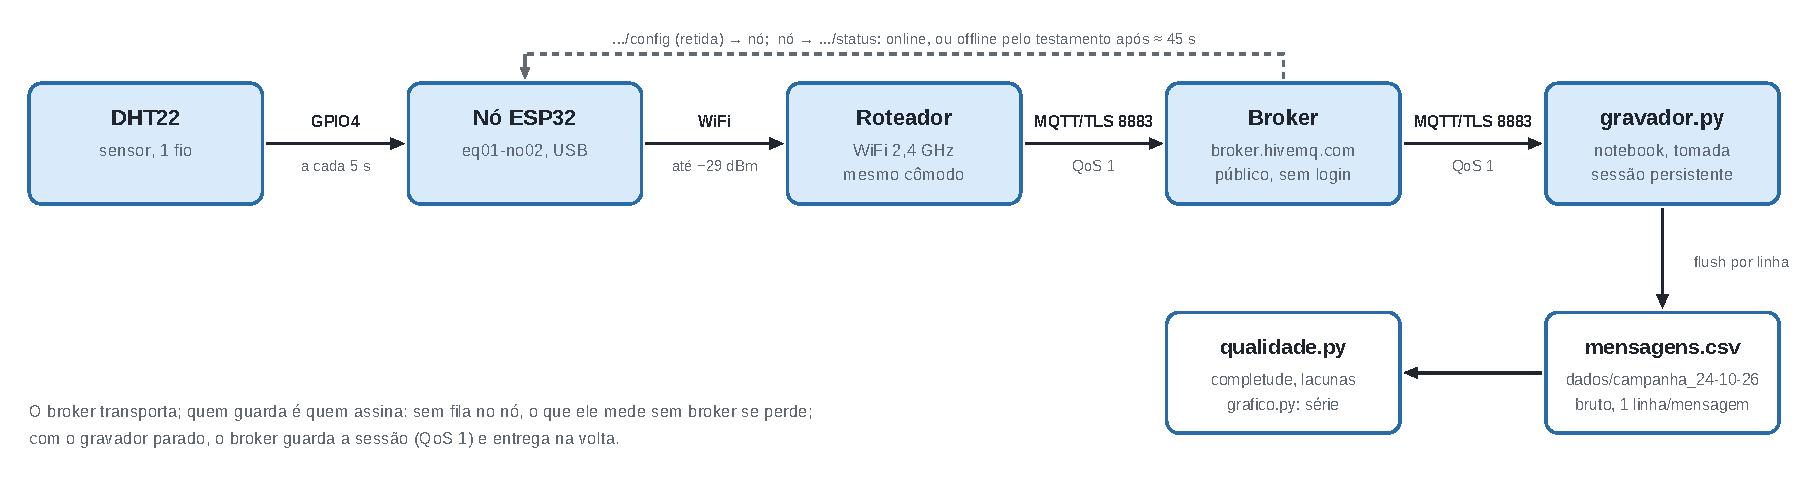
\includegraphics[width=\textwidth]{figuras/caminho-do-dado.pdf}
\caption{Caminho do dado durante a campanha de coleta}
\label{fig:caminho}
\fonte{Elaborada pela equipe.}
\end{figure}

{\footnotesize
\begin{longtable}{@{}L{2.4cm}L{3.4cm}L{3.0cm}L{5.2cm}@{}}
\caption{Onde roda cada peça, e o que acontece se ela parar}\label{tab:pecas}\\
\toprule
\textbf{Peça} & \textbf{Onde rodou} & \textbf{Alimentação} & \textbf{Se parar, o que se perde} \\
\midrule
\endfirsthead
\multicolumn{4}{@{}l}{\footnotesize\itshape Tabela~\ref{tab:pecas} --- continuação}\\
\toprule
\textbf{Peça} & \textbf{Onde rodou} & \textbf{Alimentação} & \textbf{Se parar, o que se perde} \\
\midrule
\endhead
\midrule
\multicolumn{4}{@{}r}{\footnotesize\itshape continua na próxima página}\\
\endfoot
\bottomrule
\endlastfoot
Nó ESP32       & escrivaninha, no mesmo cômodo do ar-condicionado e fora do fluxo de ar dele, na residência de João Pedro Saleh & USB & O que o nó mede enquanto está desligado nunca existe. O \texttt{status} vira \texttt{offline} em cerca de \SI{45}{\second} (\SI{46}{\second} no \CT{10}). O \emph{firmware} da campanha não tem alarme local. \\
Roteador       & o mesmo ambiente (RSSI de \SI{-15}{} a \SI{-29}{dBm}) & rede elétrica do local & O nó não alcança o \emph{broker} e, sem fila local, não mede: na queda de \SI{101}{\second} do \CT{09}, cerca de 19 leituras deixaram de existir. \\
\emph{Broker}  & público, \texttt{broker.hivemq.com}, sem autenticação & --- & Nó e gravador perdem o único elo entre eles; nada do período é guardado em lugar nenhum. \\
Gravador       & notebook de João Pedro Saleh, no mesmo local & tomada (notebook carregando) & Nada, por um tempo: com sessão persistente, \emph{client ID} fixo e QoS~1, o \emph{broker} guarda as mensagens e as entrega na volta. Na campanha, o gravador começou \SI{8,7}{\minute} depois do nó, e as 100 leituras desse intervalo chegaram juntas, com o \texttt{ts} original (\CT{12}). O \emph{broker} público não publica por quanto tempo guarda uma sessão. \\
\end{longtable}
\vspace{-0.6\baselineskip}
\fonte{Elaborada pela equipe.}
}

% ---------------------------------------------------------------------
\section{Contrato de dados}
\label{sec:contrato-dados}
\rubricaJustificativa

\begin{orientacao}
O JSON que o nó publica, na versão que rodou na campanha. Uma linha por
chave. As quatro primeiras são as da disciplina e já vêm preenchidas:
confira se o seu nó as publica exatamente assim. As demais são as
grandezas do projeto, \textbf{com a unidade no nome da chave}
(\texttt{temp\_c}, \texttt{umid\_pct}, \texttt{acel\_g}). Se o contrato
mudou durante o módulo, diga qual é a versão e o que mudou.
\end{orientacao}

{\footnotesize \setlength{\tabcolsep}{3.5pt}
\begin{longtable}{@{}L{2.3cm}L{1.8cm}L{2.2cm}L{2.4cm}L{5.4cm}@{}}
\caption{Contrato de dados da telemetria (versão 2, a da campanha)}\label{tab:contrato-dados}\\
\toprule
\textbf{Chave} & \textbf{Tipo} & \textbf{Unidade} & \textbf{Exemplo} & \textbf{Para que serve} \\
\midrule
\endfirsthead
\multicolumn{5}{@{}l}{\footnotesize\itshape Tabela~\ref{tab:contrato-dados} --- continuação}\\
\toprule
\textbf{Chave} & \textbf{Tipo} & \textbf{Unidade} & \textbf{Exemplo} & \textbf{Para que serve} \\
\midrule
\endhead
\midrule
\multicolumn{5}{@{}r}{\footnotesize\itshape continua na próxima página}\\
\endfoot
\bottomrule
\endlastfoot
\texttt{id}   & texto   & ---    & \texttt{eq01-no02} & identifica o nó (\texttt{<equipe>-<nó>}, o mesmo do tópico); parte da chave de deduplicação \\
\texttt{boot} & inteiro & ---    & ---                & \textbf{ausente na versão da campanha.} Mudaria a cada ligamento e separaria um reinício de uma perda; entra na versão~3 (\CT{11}) \\
\texttt{seq}  & inteiro & ---    & \texttt{100}       & conta as leituras e recomeça em 1 a cada ligamento; o salto denuncia a publicação que falhou, a repetição denuncia a duplicata \\
\texttt{ts}   & inteiro & s (época Unix) & \texttt{1792869010} & instante da leitura no nó (NTP), em UTC; \texttt{null} antes de sincronizar \\
\texttt{temp\_c}   & real & \si{\celsius} & \texttt{25.3} & temperatura do DHT22, leitura única por período, uma casa decimal (a resolução do sensor); ausente se a leitura falhou \\
\texttt{umid\_pct} & real & \% UR & \texttt{35.7} & umidade relativa do DHT22, uma casa decimal; ausente se a leitura falhou \\
\texttt{rssi\_dbm} & inteiro & dBm & \texttt{-17} & só quando a leitura do DHT22 falha, no lugar das duas grandezas: a mensagem continua marcando o \texttt{seq} e informa a força do sinal no ponto do nó \\
\end{longtable}
\vspace{-0.6\baselineskip}
\fonte{Elaborada pela equipe, a partir do contrato de 23/09/2026 e do
  \emph{firmware} da campanha (\texttt{wokwi/sketch/sketch.ino}, branch
  \texttt{lab3}, \emph{commit} \texttt{7b4482e}).}
}

O contrato mudou uma vez neste módulo. A versão~1, de 23/09 (Aula~10),
foi exercitada em HTTP contra um servidor de eco em 23/10: uma mensagem
dessa versão tem 73 bytes (Listagem~\ref{lst:payload}) e, enviada por
POST, voltou do servidor idêntica campo a campo. A versão~2, a que
rodou na campanha (Listagem~\ref{lst:payload2}), troca o \texttt{id}
fixo (\texttt{termo-no01}) pelo padrão \texttt{<equipe>-<nó>} do Lab~03
e, quando o DHT22 falha, publica \texttt{rssi\_dbm} no lugar das
grandezas, em vez de \texttt{null}. Foram 50 dessas mensagens nas
\num{1263} da campanha (4,0\,\%).

A versão~2 \textbf{não tem o \texttt{boot}}. Sem ele, um reinício zera o
\texttt{seq}, e uma chave de deduplicação (\texttt{id}, \texttt{seq})
descartaria leituras válidas como se fossem repetidas: aplicada aos
arquivos de 24/10, ela teria jogado fora 1 leitura da campanha e 8 dos
testes de falha, nos três reinícios. O \texttt{qualidade.py} contorna
isso separando o arquivo em trechos quando o \texttt{seq} volta a 1 ou 2
(Seção~\ref{sec:qualidade}), o que só funciona se a primeira leitura
depois do reinício chegar. A versão~3 acrescenta o \texttt{boot}, e a
chave passa a ser (\texttt{id}, \texttt{boot}, \texttt{seq}).

\begin{lstlisting}[style=terminal,
  caption={Uma mensagem real da versão 1 do contrato (sessão de 23/10, branch \texttt{apendice\_b})},
  label={lst:payload}]
{"id":"termo-no01","seq":8,"ts":1792787350,"temp_c":25.4,"umid_pct":35.5}
\end{lstlisting}

\begin{lstlisting}[style=terminal,
  caption={Duas mensagens reais da versão 2, copiadas do CSV da campanha: uma leitura normal e uma com o DHT22 em falha},
  label={lst:payload2}]
{"id":"eq01-no02","seq":100,"ts":1792869010,"temp_c":25.3,"umid_pct":35.7}
{"id":"eq01-no02","seq":7,"ts":1792868539,"rssi_dbm":-17}
\end{lstlisting}

\begin{orientacao}
Se o projeto usa (ou avaliou) BLE, transcreva também o contrato GATT de
09/10: serviço, características, formato e ordem dos bytes, escala. Se
não usa, uma frase basta: \enquote{BLE foi descartado (Tabela~\ref{tab:mudancas});
o contrato GATT está na pasta \texttt{aula13} do repositório}.
\end{orientacao}

O BLE foi avaliado e descartado (Tabela~\ref{tab:mudancas}). O contrato
GATT usado na bateria de 24/10 (branch \texttt{teste-ble}, arquivo
\texttt{firmware/comum/pacote.h}) é o da Tabela~\ref{tab:gatt}: o sensor
é o periférico e anuncia o nome \texttt{TermoStats-sensor}; o
\emph{gateway} é o central, conecta, negocia MTU de 64 (o padrão de 23
só carrega 20 bytes por notificação) e assina as notificações. O
mesmo pacote foi usado no teste de ESP-NOW, para que os dois rádios
fossem comparados com a mesma carga. O contrato GATT do exercício de
09/10 não foi arquivado no repositório; o da Tabela~\ref{tab:gatt} é o
que foi de fato exercitado em hardware, e é o que vale para este
relatório.

\begin{table}[H]
\centering
\caption{Contrato GATT da bateria de BLE (24/10)}
\label{tab:gatt}
\footnotesize
\setlength{\tabcolsep}{3.5pt}
\begin{tabular}{@{}L{3.2cm}L{2.4cm}L{2.0cm}L{6.4cm}@{}}
\toprule
\textbf{Item} & \textbf{Tipo} & \textbf{Bytes} & \textbf{Formato e escala} \\
\midrule
Serviço & UUID & --- & \texttt{6e1a0001-7d3f-4b6a-9c4e-2f1b8a5d0c01} \\
Dados (sensor $\rightarrow$ \emph{gateway}) & \emph{notify} & 25 & \texttt{6e1a0002-7d3f-4b6a-9c4e-2f1b8a5d0c01}; estrutura empacotada, \emph{little-endian} \\
ACK (\emph{gateway} $\rightarrow$ sensor) & \emph{write} sem resposta & 9 & \texttt{6e1a0003-7d3f-4b6a-9c4e-2f1b8a5d0c01}; \texttt{tipo}, \texttt{seq} confirmado e \texttt{t\_envio\_us} ecoado \\
\midrule
\texttt{tipo} & \texttt{uint8} & 1 & 1 = dado, 2 = ACK \\
\texttt{seq} & \texttt{uint32} & 4 & avança a cada \SI{100}{\milli\second}, conectado ou não: o buraco é a perda \\
\texttt{t\_envio\_us} & \texttt{uint32} & 4 & \texttt{micros()} do sensor no envio \\
\texttt{rtt\_us}, \texttt{seq\_rtt} & \texttt{uint32} & 4 + 4 & ida e volta medida no último ACK, e a qual \texttt{seq} ela se refere \\
\texttt{tx\_falhas} & \texttt{uint32} & 4 & pacotes não enviados desde o \emph{boot} \\
\texttt{temp\_c\_x10} & \texttt{int16} & 2 & \si{\celsius} $\times$ 10 (\num{26.1} $\rightarrow$ 261); \texttt{INT16\_MIN} = leitura inválida \\
\texttt{umid\_pct\_x10} & \texttt{uint16} & 2 & \% UR $\times$ 10; \texttt{UINT16\_MAX} = leitura inválida \\
\bottomrule
\end{tabular}
\fonte{Elaborada pela equipe, a partir de \texttt{firmware/comum/pacote.h} (branch \texttt{teste-ble}).}
\end{table}

Só os dois últimos campos (4 bytes) são dado do projeto; os outros 21
existem para medir o enlace. Em produção, com \texttt{boot} e
\texttt{seq} de 2 bytes, o pacote cabe em 8 bytes, o tamanho usado na
conta do ar da Tabela~\ref{tab:mudancas}.

% ---------------------------------------------------------------------
\section{Contrato de tópicos e garantias de entrega}
\label{sec:topicos}
\rubricaJustificativa

\begin{orientacao}
O contrato de 29/09, na versão da campanha. A coluna \enquote{Por quê}
é a que o docente lê primeiro: uma frase por linha. Lembretes da Aula 11:
o QoS efetivo de uma entrega é o \textbf{menor} entre o de quem publica e
o de quem assina; QoS~1 pode entregar duas vezes, e é o \texttt{seq} que
permite descartar a duplicata; telemetria retida faz um painel recém-aberto
mostrar uma leitura velha como se fosse atual.
\end{orientacao}

{\scriptsize \setlength{\tabcolsep}{3pt}
\begin{longtable}{@{}L{3.6cm}L{1.9cm}C{0.8cm}C{1.1cm}L{2.4cm}L{4.0cm}@{}}
\caption{Contrato de tópicos MQTT}\label{tab:topicos}\\
\toprule
\textbf{Tópico} & \textbf{Direção} & \textbf{QoS} & \textbf{Retido?} & \textbf{Quem assina} & \textbf{Por quê} \\
\midrule
\endfirsthead
\multicolumn{6}{@{}l}{\footnotesize\itshape Tabela~\ref{tab:topicos} --- continuação}\\
\toprule
\textbf{Tópico} & \textbf{Direção} & \textbf{QoS} & \textbf{Retido?} & \textbf{Quem assina} & \textbf{Por quê} \\
\midrule
\endhead
\midrule
\multicolumn{6}{@{}r}{\footnotesize\itshape continua na próxima página}\\
\endfoot
\bottomrule
\endlastfoot
\texttt{ufpi-iot26/\allowbreak eq01/\allowbreak no02/\allowbreak telemetria} & nó $\rightarrow$ \emph{broker} & 1 & não & gravador & QoS~1 garante a entrega nas duas pernas; a cópia que ele pode gerar sai pela chave (\texttt{id}, \texttt{seq}) dentro de cada trecho entre reinícios, enquanto não houver \texttt{boot}. Retida, faria um painel recém-aberto mostrar uma leitura velha como atual. \\
\texttt{ufpi-iot26/\allowbreak eq01/\allowbreak no02/\allowbreak status}     & nó $\rightarrow$ \emph{broker} (e testamento) & 1 & sim & gravador; MQTT Explorer, para ver ao vivo & Retido, quem chega depois vê o estado atual na hora; o testamento publica \texttt{offline} quando o nó cai sem avisar. \\
\texttt{ufpi-iot26/\allowbreak eq01/\allowbreak no02/\allowbreak config}     & \emph{broker} $\rightarrow$ nó & 1 & sim & o nó & \texttt{\{\textquotedbl periodo\_s\textquotedbl:N\}}. Retida, o nó que reinicia recebe a configuração logo ao conectar, sem perguntar; mensagem vazia retida volta ao padrão (\SI{5}{\second}). Não foi usada na campanha. \\
\end{longtable}
\vspace{-0.6\baselineskip}
\fonte{Elaborada pela equipe, a partir do contrato de 29/09/2026. Na
  campanha, o nó da placa foi o \texttt{no02}; o \texttt{no01} fica
  reservado para o Wokwi, para que os dois nunca usem o mesmo
  \emph{client ID}.}
}

\begin{orientacao}
Depois da tabela, as quatro decisões que transformam um nó que publica
num nó que forma um conjunto de dados. Cada uma com o número que a
sustenta. Se alguma delas for importante o bastante para o projeto,
promova-a a uma caixa \DP{n}.
\end{orientacao}

\noindent O protocolo da campanha é o MQTT do Lab~03. Comparado a
WebSocket e Firebase no ESP32-C3, sob as mesmas condições, ele teve
desempenho equilibrado e o uso de banda mais eficiente em redes
restritas \cite{yamin2026mqttwsfirebase}; e a sessão persistente, o
QoS e o testamento, que as quatro decisões abaixo usam, são do próprio
protocolo.

\begin{description}[style=unboxed, leftmargin=0pt, font=\normalfont\bfseries]
  \item[1. Sessão persistente ou limpa, no nó e no gravador.]\hfill\\
    Persistente nos dois, com \emph{client ID} fixo:
    \texttt{ufpi-iot26-eq01-no02} no nó e \texttt{ufpi-iot26-eq01-gravador}
    no gravador. É a combinação de sessão persistente, mesmo \emph{client
    ID} e QoS~1 que faz o \emph{broker} guardar as leituras enquanto o
    gravador está parado: na campanha, o gravador foi ligado
    \SI{8,7}{\minute} depois do nó, e as 100 leituras desse intervalo
    chegaram em \SI{3}{\second}, com o \texttt{ts} original. Dois clientes
    com o mesmo ID derrubam um ao outro; por isso a placa e o Wokwi nunca
    usam o mesmo nome de nó.
  \item[2. O que o nó faz com as leituras quando o broker está fora de alcance.]\hfill\\
    Nada: o \emph{firmware} da campanha não tem fila local. Sem
    \emph{broker}, a leitura não é feita, e o \texttt{seq} não avança. Na
    queda de WiFi do \CT{09} (\SI{101}{\second}), cerca de 19 leituras
    deixaram de existir, e o \texttt{seq} pulou só 1; na campanha,
    faltaram cerca de 740 leituras, e o \texttt{seq} acusou 2. A lacuna
    não aparece como salto de \texttt{seq}; só aparece na completude
    (Seção~\ref{sec:qualidade}). Com uma fila de 120 leituras, que em
    binário (\texttt{ts}, \texttt{seq} e as duas grandezas, 12 bytes cada)
    ocupam menos de 1,5\,kB de RAM, o nó cobriria
    \SI{10}{\minute} sem \emph{broker} no período de \SI{5}{\second}, ou 20
    horas no período de \SI{600}{\second} do \RF{01}. Essa fila é a
    principal mudança de \emph{firmware} para o próximo ciclo.
  \item[3. Keepalive e testamento.]\hfill\\
    \emph{Keepalive} de \SI{30}{\second}: um nó que morre sem avisar
    aparece como \texttt{offline} cerca de \SI{45}{\second} depois da
    última mensagem dele (\SI{46}{\second} no \CT{10}). No
    \emph{firmware} da campanha, o laço não tem nenhum \texttt{delay()}
    longo: a leitura do DHT22 é única, e o período é contado com
    \texttt{millis()}. A leitura filtrada da AP1 com o pulso de alarme
    deixaria o laço cerca de \SI{11,4}{\second} sem chamar
    \texttt{mqtt.loop()}, ainda dentro do limite, quando as duas versões
    forem unidas.
  \item[4. Segurança mínima.]\hfill\\
    TLS na porta 8883 nas duas pontas, mas \textbf{sem autenticação}: a
    campanha usou o \emph{broker} público \texttt{broker.hivemq.com}, sem
    usuário nem senha, e qualquer pessoa pode ler e publicar em
    \texttt{ufpi-iot26/eq01/\#}. O público foi usado porque os testes e a
    campanha foram feitos remotamente, na residência de um integrante,
    e o nó e o gravador foram configurados sem as credenciais da equipe
    no \emph{broker} da turma: o \texttt{secrets.example.h} e o README da
    \texttt{lab3} já trazem \texttt{broker.hivemq.com}, porta 8883, sem
    usuário, e o gravador foi alterado para aceitar a conexão sem login
    (Seção~\ref{sec:firmware-com}). Foi uma escolha de praticidade, não
    de projeto, e tem o custo que a Aula~11 aponta: num \emph{broker}
    público, qualquer um lê a telemetria e pode escrever no
    \texttt{config} do nó. Nenhuma mensagem chegou fora dos tópicos
    \texttt{status} e \texttt{telemetria} do nó. O \texttt{secrets.h}
    está no \texttt{.gitignore}, e o repositório só tem o
    \texttt{secrets.example.h}: nenhum \emph{commit}, em nenhuma branch,
    contém um \texttt{secrets.h} (conferido com \texttt{git log -{}-all}).
    O gravador confere o certificado do \emph{broker} com as autoridades
    certificadoras do sistema; o nó, não (\texttt{setInsecure()}): a
    conexão é cifrada, mas um servidor falso na mesma rede poderia se
    passar pelo \emph{broker}. Com o \emph{broker} da turma, ele
    receberia também a senha da equipe. Conferir o certificado do
    servidor e manter as credenciais fora do código são as medidas
    básicas que os guias de segurança para ESP32 apontam
    \cite{wavtron2025iotsecurity}; a campanha cumpriu a segunda, e não
    a primeira. É uma limitação declarada
    (Cap.~\ref{cap:conclusao}).
\end{description}

% ---------------------------------------------------------------------
\section{Custo real da comunicação}
\label{sec:custo-radio}
\rubricaJustificativa

\begin{orientacao}
Na AP1, a linha do rádio do orçamento de energia entrou como
\estimativa. Agora ela é medida. O que se mede com a placa é o
\textbf{tempo}: quanto o nó leva para associar ao WiFi, obter endereço,
conectar ao \emph{broker} e publicar (a medição da Aula 10). A
\textbf{corrente} vem do medidor USB, se a equipe tiver um, ou da folha de
dados; declare qual. O Wokwi não simula corrente.

Atualize o Apêndice~\ref{ap:energia} com estes números e diga o que mudou
na autonomia.
\end{orientacao}

\begin{table}[H]
\centering
\caption{Linha do rádio: estimada na AP1 \emph{versus} medida na AP2}
\label{tab:custo-radio}
\footnotesize
\setlength{\tabcolsep}{3.5pt}
\begin{tabular}{@{}L{3.6cm}R{1.9cm}R{1.9cm}L{3.4cm}L{3.0cm}@{}}
\toprule
\textbf{Etapa} & \textbf{Estimado (AP1)} & \textbf{Medido (AP2)} & \textbf{Como foi medido} & \textbf{Origem da corrente} \\
\midrule
Associação WiFi + DHCP      & --- & 1,74\,s & \texttt{millis()} nos eventos do WiFi; mediana de 10 ciclos (0,22 + 1,52) & \multirow{4}{3.0cm}{\bancada: medidor USB na rajada de 23/10, \SI{300}{\milli\ampere}} \\
Conexão TLS                 & --- & 1,04\,s & mediana de 10 ciclos HTTPS (máx. \SI{7,0}{\second}); servidor de eco, não o \emph{broker} & \\
Publicação                  & --- & 0,23\,s & requisição HTTP, mediana de 10 ciclos & \\
Ciclo completo              & --- & 2,27 / 3,16\,s & mediana HTTP / HTTPS; pior HTTP: \SI{2,48}{\second} & \\
Conectado e ocioso          & --- & não medido & --- & --- \\
\midrule
\textbf{Rádio por dia}      & 0 (não orçado) & 29,7\,mA$\cdot$h & \multicolumn{2}{L{6.6cm}}{pior ciclo HTTP; com TLS (mediana), $\approx$37,9 (Apêndice~\ref{ap:energia})} \\
\bottomrule
\end{tabular}
\fonte{Elaborada pela equipe. A AP1 não chegou a estimar a linha do
  rádio: no orçamento entregue, o estado \emph{transmite} constava como
  \enquote{não se aplica neste ciclo} (Apêndice~\ref{ap:energia}), e o
  total de \SI{69.4}{\mAh}/dia cobria apenas o sensoriamento.}
\end{table}

Os tempos foram medidos com HTTP, e não com MQTT. Uma revisão
sistemática de estudos com ESP32 encontrou, para o MQTT, latência menor,
menos \emph{overhead} com TLS e consumo de 6 a 8\,\% menor que o do
HTTP \cite{adriansyah2026mqtt}; por isso a linha do rádio medida em
HTTP tende a ser conservadora para o nó MQTT. Os tempos vêm da
ferramenta da Aula~10 (branch \texttt{apendice\_b}),
medidos na placa em 23/10 com o ciclo que um nó em \emph{deep sleep}
pagaria a cada despertar: rádio desligado, associa, obtém IP, resolve o
nome, conecta, publica e desliga. Três coisas saem deles:

\begin{itemize}
  \item \textbf{Quem domina o ciclo é o DHCP}, com \SI{1,52}{\second} dos
    \SI{2,27}{\second} (67\,\%). A publicação em si custa
    \SI{0,23}{\second}. Um IP fixo cortaria a maior parcela do ciclo, ao
    preço de configurar o endereço em cada nó.
  \item \textbf{O TLS acrescenta cerca de \SI{0,8}{\second} na mediana},
    e a cauda é longa: em 3 dos 10 ciclos HTTPS a conexão levou de 3,8 a
    \SI{7,0}{\second}. A conexão TLS foi medida com um servidor de eco
    (\texttt{httpbin.org}), não com o \emph{broker} da campanha. A
    conexão ao \emph{broker} não foi cronometrada; na campanha, o
    caminho inteiro, da medição até a linha no CSV, levou
    \SI{0,8}{\second} na mediana e \SI{1,9}{\second} no p95.
  \item \textbf{O rádio falha às vezes.} Em 2 dos 26 ciclos HTTP, a
    conexão esgotou o tempo de \SI{3}{\second} e o ciclo terminou sem
    resposta, o que justifica a fila local (\RF{06}).
\end{itemize}

A corrente é a da placa inteira, lida no medidor USB na entrada de
\SI{5}{\volt} durante a rajada de \SI{30}{\second} da ferramenta
(12 ciclos HTTP seguidos, tecla \texttt{r}, sessão de 23/10). Ela inclui
o regulador e o conversor USB-serial, e superestima o que um módulo sem
esses componentes consumiria. A leitura do medidor não passou pela
placa: foi informada ao processamento (\texttt{python -m gravador
processar -{}-corrente 300}), e por isso o log da sessão só mostra o
valor que a ferramenta guardava antes, \SI{120}{\milli\ampere}, a
estimativa de 09/09 do \texttt{config.h}. Com ela, a linha do rádio
cairia para \SI{11,9}{\mAh}/dia.

Se o nó ficar sempre conectado (\DP{6}), esta conta muda de natureza: o
que pesa passa a ser a corrente do nó conectado e ocioso, que não foi
medida, e não o ciclo de conexão.

% ---------------------------------------------------------------------
\section{A campanha de coleta}
\label{sec:campanha}
\rubricaRobustez

\begin{orientacao}
\textbf{A disciplina não fixa uma duração mínima para a campanha.} A
equipe declara quanto coletou e justifica por que é suficiente para o
que pretende fazer no Módulo 3, ou admite que não é. O critério é o
fenômeno, não o relógio: se a grandeza tem ciclo diário (temperatura de
um galpão), uma tarde não mostra o ciclo; se o evento de interesse é
raro (a porta que abre, o animal que deita), conte quantas vezes ele
aconteceu durante a coleta.

As \enquote{leituras esperadas} saem de uma conta, não do arquivo:
duração em que o nó deveria estar publicando $\div$ período de
amostragem. É contra esse número que a completude da
Seção~\ref{sec:qualidade} é calculada.

O diário da campanha (o que aconteceu, quando, como a equipe soube, o
que fez) vai no Apêndice~\ref{ap:campanha}.
\end{orientacao}

{\footnotesize
\begin{longtable}{@{}L{5.0cm}L{9.0cm}@{}}
\caption{Ficha da campanha de coleta}\label{tab:campanha}\\
\toprule
\textbf{Item} & \textbf{Valor} \\
\midrule
\endfirsthead
\multicolumn{2}{@{}l}{\footnotesize\itshape Tabela~\ref{tab:campanha} --- continuação}\\
\toprule
\textbf{Item} & \textbf{Valor} \\
\midrule
\endhead
\midrule
\multicolumn{2}{@{}r}{\footnotesize\itshape continua na próxima página}\\
\endfoot
\bottomrule
\endlastfoot
Local de instalação do nó                & em cima de uma escrivaninha, no mesmo cômodo do ar-condicionado, fora do fluxo de ar dele; o roteador no mesmo ambiente (RSSI de \SI{-15}{} a \SI{-29}{dBm}), na residência de João Pedro Saleh; só ele esteve no cômodo durante a coleta. Não foi na farmácia porque o acesso é restrito e exigiria sanitização e permissão dos proprietários \\
Início e fim (data e hora)               & 24/10/2026, das 16:01:32 (primeira leitura do nó ligado para a campanha, logo depois dos testes de falha; reiniciado às 16:01:36) às 18:48:26 (gravador parado), pelo diário do Apêndice~\ref{ap:campanha}; as pontas coincidem com a primeira e a última leitura \\
Duração total                            & 2,78\,h (\SI{166,9}{\minute}) \\
Período de amostragem                    & \SI{5}{\second}, o padrão do \emph{firmware} do Lab~03 (o \RF{01} pede \SI{600}{\second}) \\
Leituras esperadas (duração $\div$ período) & \num{2003} ($\num{166.9} \times 60 \div 5 + 1$) \\
Número de nós                            & 1 (\texttt{eq01-no02}) \\
Onde rodou o gravador                    & notebook de João Pedro Saleh, na tomada, no mesmo local; ligado às 16:10:14 e parado às 18:48:26 \\
Como a equipe acompanhou a coleta        & terminal do gravador, com cada mensagem impressa ao chegar, acompanhado por João Pedro Saleh: a fase de quedas foi vista durante a coleta e comprovada depois no CSV. Os eventos do ambiente foram anotados por ele, com a hora (Apêndice~\ref{ap:campanha}). Nenhum aviso automático de queda \\
Por que esta duração basta para a AP3    & Basta para descrever um evento: o desligamento do ar-condicionado às 16:35, com 33 minutos de ar ligado antes e 2\,h\,13\,min depois. Não basta para o ciclo diário, para a madrugada nem para repetir o evento: é uma tarde só (Seção~\ref{sec:dataset}) \\
\end{longtable}
\vspace{-0.6\baselineskip}
\fonte{Elaborada pela equipe, a partir de
  \texttt{dados/campanha\_24-10-26/resultados.md} (branch \texttt{lab3}).}
}

A campanha foi feita em 24/10, e não ao longo da semana de 19 a 25/10, e
não no cenário de referência (Seção~\ref{sec:local}). Ela durou uma
tarde: o nó, o roteador e o notebook do gravador estavam na residência
de um integrante, que acompanhou toda a coleta, e a coleta terminou
quando ele encerrou o gravador, sem se estender pela noite. É a
principal limitação do conjunto (Seção~\ref{sec:dataset} e
Cap.~\ref{cap:conclusao}). O período de
\SI{5}{\second} é 120 vezes mais curto que o do \RF{01}: ele deu à
análise de conectividade \num{2003} leituras esperadas em menos de três
horas, mas, reamostrada a \SI{600}{\second}, a mesma tarde teria só 17
leituras. O nó ficou ligado à USB, sem \emph{deep sleep} (\DP{6}), e
nada desta campanha mede a autonomia.

% ---------------------------------------------------------------------
\section{Qualidade do conjunto de dados}
\label{sec:qualidade}
\rubricaRobustez

\begin{orientacao}
Os números saem do \texttt{qualidade.py} rodado sobre o arquivo final da
campanha, e a saída completa, sem edição, vai no
Apêndice~\ref{ap:campanha}. Aqui entram os números e, para cada um,
\textbf{a explicação}. Faltas explicadas valem mais do que zero faltas
sem explicação: o \texttt{status} e o \texttt{boot} quase sempre dizem
o que aconteceu.

A completude é
\[
  \text{completude}\,[\%] = \frac{\text{leituras únicas recebidas}}
                                 {\text{leituras esperadas}} \times 100.
\]
\end{orientacao}

{\footnotesize
\begin{longtable}{@{}L{4.6cm}R{2.0cm}L{7.4cm}@{}}
\caption{Qualidade do conjunto de dados coletado}\label{tab:qualidade}\\
\toprule
\textbf{Métrica} & \textbf{Valor} & \textbf{O que explica o valor} \\
\midrule
\endfirsthead
\multicolumn{3}{@{}l}{\footnotesize\itshape Tabela~\ref{tab:qualidade} --- continuação}\\
\toprule
\textbf{Métrica} & \textbf{Valor} & \textbf{O que explica o valor} \\
\midrule
\endhead
\midrule
\multicolumn{3}{@{}r}{\footnotesize\itshape continua na próxima página}\\
\endfoot
\bottomrule
\endlastfoot
Leituras esperadas                    & \num{2003} & Tabela~\ref{tab:campanha}: a janela em que o nó deveria publicar, do diário, dividida pelo período de \SI{5}{\second} \\
Leituras recebidas                    & \num{1263} & \texttt{seq} 33 a \num{1264}, com um reinício logo no início. Destas, \num{1213} trazem o DHT22 e 50 (4,0\,\%) só o \texttt{rssi\_dbm}, porque a leitura do sensor falhou \\
Faltam (o \texttt{seq} pulou)         & 2 & \texttt{seq} 193 e 333: publicações tentadas que falharam. O \texttt{seq} não mede a perda desta campanha (ver abaixo) \\
Repetidas (descartadas)               & 0 & nenhuma cópia do QoS~1 chegou ao CSV \\
Reinícios do nó                       & 1 & às 16:01:36, o reinício que abriu a campanha (\texttt{seq} 33 $\rightarrow$ 1) \\
Leituras sem hora (\texttt{ts null})  & 0 & o NTP acertou antes da primeira publicação (\CT{13}) \\
Atraso chegada $-$ \texttt{ts} (mediana · máximo) & \SI{1}{\second} · \SI{523}{\second} & o máximo é o lote guardado pelo \emph{broker} enquanto o gravador não estava ligado; sem ele, mediana de \SI{0,8}{\second}, p95 de \SI{1,9}{\second} e máximo de \SI{6,9}{\second} \\
Mensagens fora do contrato            & 0 & todas com \texttt{id}, \texttt{seq} e \texttt{ts}; nenhuma mensagem fora dos tópicos do nó, no \emph{broker} público \\
Quedas de conexão (\texttt{offline})  & 764 & testamentos publicados pelo \emph{broker}, contra 570 \texttt{online}; 695 delas entre 16:30 e 18:10 \\
\midrule
\textbf{Completude}                   & \textbf{63,1\,\%} & \num{1263} únicas $\div$ \num{2003} esperadas; 60,6\,\% contando só as leituras com o DHT22 \\
\end{longtable}
\vspace{-0.6\baselineskip}
\fonte{Saída do \texttt{qualidade.py} sobre
  \texttt{dados/campanha\_24-10-26/mensagens.csv}
  (Listagem~\ref{lst:qualidade}); o atraso sem o lote inicial e as
  quedas de conexão foram contados à parte, sobre o mesmo CSV.}
}

\textbf{O \texttt{seq} não mede a perda desta campanha.} Ele acusa 2
leituras faltando, e faltam cerca de 740. Sem fila local, o nó
desconectado não mede, e o \texttt{seq} não avança; só a conta pelo
tempo mostra o buraco.

\textbf{A completude não caiu por igual.} A campanha teve três fases
nítidas (Tabela~\ref{tab:fases} e Figura~\ref{fig:resultado}). Nas duas
estáveis, o nó ficou perto de 96\,\%; a perda que sobra nelas vem de
segundos perdidos em reconexões. De 18:20 ao fim, a completude foi de
100\,\%. Entre 16:30 e 18:10, o nó conectava e caía em ciclo. Na
campanha inteira, das 545 conexões com \texttt{online} seguido de
\texttt{offline}, a mediana durou
\SI{3}{\second}, e 65\,\% duraram menos que os \SI{5}{\second} de um
período; 195 vezes a conexão caiu antes mesmo de o \texttt{online} ser
publicado.

\begin{table}[H]
\centering
\caption{As três fases de conectividade da campanha}
\label{tab:fases}
\footnotesize
\begin{tabular}{@{}L{3.0cm}L{2.6cm}R{2.8cm}R{2.0cm}R{2.0cm}@{}}
\toprule
\textbf{Fase} & \textbf{Horário} & \textbf{Recebidas / esperadas} & \textbf{Completude} & \textbf{\texttt{offline}} \\
\midrule
A $\cdot$ estável   & 16:01 a 16:30 & 329 / 344   & 95,6\,\% & $\approx$50 \\
B $\cdot$ degradada & 16:30 a 18:10 & 488 / \num{1210} & 40,3\,\% & 695 \\
C $\cdot$ estável   & 18:10 a 18:48 & 446 / 465   & 95,9\,\% & 19 \\
\bottomrule
\end{tabular}
\fonte{\texttt{dados/campanha\_24-10-26/resultados.md}, contagem por
  janelas de \SI{10}{\minute} (totais aproximados).}
\end{table}

\textbf{Hipótese para a fase B: o \emph{timeout} de \SI{1}{\second} da
biblioteca MQTT.} A biblioteca \texttt{256dpi/MQTT} espera no máximo
\SI{1000}{\milli\second} pela resposta do \emph{broker} em cada operação
(CONNACK, PUBACK do QoS~1, SUBACK) e, se o tempo estoura, fecha a
conexão. O \emph{broker} vê a conexão cair sem DISCONNECT e publica o
testamento; o nó reconecta, publica \texttt{online} com QoS~1, espera o
PUBACK e estoura de novo. Um \emph{broker} público fora do Brasil e uma
rede residencial carregada tornam plausíveis picos de ida e volta acima
de \SI{1}{\second}. O rádio não é suspeito: o RSSI ficou entre
\SI{-15}{} e \SI{-29}{dBm}. A hipótese não explica por que a degradação
começou perto das 16:30 e acabou perto das 18:10, e a latência até o
\emph{broker} não foi medida. Para confirmá-la: procurar no log serial
as linhas \texttt{<- FALHOU} e o código de erro do \texttt{connect()}, se
o monitor ficou aberto, e repetir a coleta com
\texttt{mqtt.setTimeout(5000)}, comparando a contagem de \texttt{offline}.
O \emph{firmware} descrito neste relatório é o que rodou, sem essa
mudança.

O \texttt{qualidade.py} usado é o do Lab~03 com mudanças da equipe
(Seção~\ref{sec:firmware-com}): além de recebidas, faltas, repetidas,
reinícios, \texttt{ts} nulo e atraso, que já vinham do docente, ele
calcula as leituras esperadas pela conta $(\text{fim} - \text{início})
\div \text{período} + 1$, a completude e as lacunas maiores que
$1{,}5 \times$ o período. Dois limites que ficaram da versão original
importam para ler a tabela:

\begin{itemize}
  \item \textbf{Ele reconhece um reinício pelo \texttt{seq} voltando a 1
    ou 2, e não pelo \texttt{boot}}, que a versão~2 do contrato não tem.
    Se as primeiras leituras depois de um reinício se perderem, o
    reinício passa despercebido e vira faltas ou repetidas falsas. Nos
    três reinícios de 24/10, a primeira leitura chegou, e o script
    acertou.
  \item \textbf{As opções \texttt{-{}-de} e \texttt{-{}-ate} comparam só
    a hora, sem a data.} Numa campanha que passe da meia-noite, a janela
    pega o mesmo horário dos dois dias. A campanha de 24/10 coube numa
    tarde, e o relatório roda sobre o arquivo inteiro, sem janela.
\end{itemize}

\begin{table}[H]
\centering
\caption{Lacunas do conjunto de dados}
\label{tab:lacunas}
\footnotesize
\setlength{\tabcolsep}{3.5pt}
\begin{tabular}{@{}L{2.4cm}L{2.4cm}R{1.6cm}R{1.6cm}L{3.0cm}L{2.9cm}@{}}
\toprule
\textbf{Início} & \textbf{Fim} & \textbf{Duração} & \textbf{Leituras perdidas} & \textbf{Causa} & \textbf{Tratamento} \\
\midrule
17:52:52 & 18:02:22 & \SI{570}{\second} & $\approx$113 & conexões ao \emph{broker} caindo em segundos (fase B) & mantida como lacuna; nada é interpolado \\
18:02:22 & 18:06:28 & \SI{246}{\second} & $\approx$48 & idem & idem \\
17:46:13 & 17:50:02 & \SI{229}{\second} & $\approx$45 & idem & idem \\
17:50:02 & 17:52:52 & \SI{170}{\second} & $\approx$33 & idem & idem \\
16:49:02 & 16:51:51 & \SI{169}{\second} & $\approx$33 & idem & idem \\
\midrule
\multicolumn{2}{@{}l}{outras 133 lacunas} & \SI{3003}{\second} & $\approx$470 & reconexões, quase todas na fase B & idem \\
\midrule
\multicolumn{2}{@{}l}{\textbf{total: 138 lacunas}} & \SI{4387}{\second} & $\approx$740 & & \\
\bottomrule
\end{tabular}
\fonte{Saída do \texttt{qualidade.py} (lacunas maiores que $1{,}5 \times$
  \SI{5}{\second}, Listagem~\ref{lst:qualidade}). O pior trecho foi de
  17:46 a 18:10: 13 leituras em \SI{24}{\minute}.}
\end{table}

% ---------------------------------------------------------------------
\section{Descrição do conjunto de dados}
\label{sec:dataset}
\rubricaRobustez

\begin{orientacao}
É a ficha que a equipe vai abrir em novembro, no Módulo 3, sem lembrar
de nada do que aconteceu em outubro. Uma linha por coluna do arquivo
\textbf{final} (depois da limpeza, se houve), com a faixa que de fato
apareceu nos dados, não a faixa do sensor. Diga onde o arquivo está no
repositório, o tamanho e o formato, e se ele é o bruto do gravador ou um
derivado (e, nesse caso, qual \emph{script} gera um a partir do outro).
\end{orientacao}

{\footnotesize \setlength{\tabcolsep}{3.5pt}
\begin{longtable}{@{}L{2.6cm}L{1.8cm}L{2.2cm}L{2.8cm}L{4.6cm}@{}}
\caption{Descrição do conjunto de dados}\label{tab:dataset}\\
\toprule
\textbf{Campo} & \textbf{Tipo} & \textbf{Unidade} & \textbf{Faixa observada} & \textbf{Observação} \\
\midrule
\endfirsthead
\multicolumn{5}{@{}l}{\footnotesize\itshape Tabela~\ref{tab:dataset} --- continuação}\\
\toprule
\textbf{Campo} & \textbf{Tipo} & \textbf{Unidade} & \textbf{Faixa observada} & \textbf{Observação} \\
\midrule
\endhead
\midrule
\multicolumn{5}{@{}r}{\footnotesize\itshape continua na próxima página}\\
\endfoot
\bottomrule
\endlastfoot
\texttt{t\_chegada} & real & s (época Unix) & \texttt{1792869014.986} a \texttt{1792878506.576} (16:10:14 a 18:48:26) & instante em que o gravador recebeu a mensagem (relógio do computador), em milissegundos \\
\texttt{chegada} & texto & HH:MM:SS & --- & a mesma hora, legível; sem a data \\
\texttt{topico} & texto & --- & \texttt{ufpi-iot26/eq01/no02/telemetria} (\num{1263} linhas) e \texttt{ufpi-iot26/eq01/no02/status} (\num{1334}) & separa as leituras dos registros de estado \\
\texttt{retido} & inteiro & --- & 0 ou 1 (uma linha com 1) & 1 quando o \emph{broker} entregou uma mensagem retida (o \texttt{status} ao conectar) \\
\texttt{payload} & texto & --- & \texttt{online}, \texttt{offline} ou JSON & a mensagem como chegou; nas linhas de telemetria, o JSON da Tabela~\ref{tab:contrato-dados} \\
\quad\texttt{seq} & inteiro & --- & 1 a \num{1264} (e 33, antes do reinício) & contador do nó \\
\quad\texttt{ts} & inteiro & s (época Unix) & \texttt{1792868492} a \texttt{1792878506} (16:01:32 a 18:48:26) & instante da leitura no nó; nenhum nulo \\
\quad\texttt{temp\_c} & real & \si{\celsius} & 24,0 a 30,7 & DHT22, leitura única, resolução de \SI{0,1}{\celsius}; média de 27,9 e desvio de \SI{2,5}{\celsius} \\
\quad\texttt{umid\_pct} & real & \% UR & 34,2 a 41,2 & DHT22, leitura única, resolução de 0,1\,\%; média de 38,2 e desvio de 2,2 \\
\quad\texttt{rssi\_dbm} & inteiro & dBm & \num{-29} a \num{-15} (50 linhas) & só nas leituras em que o DHT22 falhou \\
\end{longtable}
\vspace{-0.6\baselineskip}
\fonte{Elaborada pela equipe, a partir do CSV da campanha.}
}

\noindent Arquivo: \texttt{dados/campanha\_24-10-26/mensagens.csv}, o
bruto do gravador, sem nenhuma edição e sem versão limpa \quad Tamanho:
261\,kB \quad Linhas: \num{2597} mais o cabeçalho \quad \emph{Commit}:
o da entrega, marcado com a \emph{tag} \texttt{ap2} (Seção~\ref{sec:repositorio}),
com o arquivo idêntico ao do \texttt{7b4482e} (branch \texttt{lab3}),
onde foi gravado. Na mesma pasta estão a saída
do \texttt{qualidade.py}, o gráfico da Figura~\ref{fig:resultado}
(gerado por \texttt{gravador/grafico.py}) e o \texttt{resultados.md}. A
temperatura nunca variou mais que \SI{0,2}{\celsius}, nem a umidade
mais que 0,5 ponto, entre duas leituras consecutivas: não há salto
espúrio, e os degraus da série são a resolução do sensor.

\begin{enumerate}[label=\arabic*.]
  \item \textbf{O que a equipe quer que um modelo aprenda com estes
    dados?} Detectar uma falha de climatização (o ar-condicionado que
    desliga ou para) pela forma da curva de temperatura e umidade,
    antes de a leitura sair da faixa. É o alvo da AP3.
  \item \textbf{O conjunto tem exemplos suficientes disso?} Não. A
    campanha tem \textbf{um} evento anotado, o desligamento do
    ar-condicionado às 16:35, com a resposta clara: $+$\SI{2}{\celsius}
    em \SI{6}{\minute}. Um exemplo serve para descrever o fenômeno e
    escolher a janela, mas não para treinar nem validar um
    classificador; faltam mais desligamentos anotados, em dias e horários
    diferentes, e trechos longos sem evento.
\end{enumerate}

\begin{orientacao}
Feche a seção com duas respostas curtas, que ligam este ciclo ao seguinte:

\begin{enumerate}[label=\arabic*.]
  \item \textbf{O que a equipe quer que um modelo aprenda com estes
    dados?} Classificar estados, prever uma grandeza, detectar uma
    anomalia. Uma frase.
  \item \textbf{O conjunto tem exemplos suficientes disso?} Quantas vezes
    o evento de interesse aconteceu durante a coleta, e se a equipe
    anotou quando (o registro de eventos do Apêndice~\ref{ap:campanha}).
    Sem essa anotação, a rotulagem de novembro vira adivinhação.
\end{enumerate}
\end{orientacao}

\fi

% Capítulo que só existe na AP3 (dados, modelo e inferência embarcada)
\ifnum\value{ciclo}>2\relax
  % =====================================================================
%  Capítulo 6 — Dados, modelo e inferência embarcada (só na AP3)
% =====================================================================
\chapter{Pipeline de dados, modelo e inferência embarcada}
\label{cap:modelo}
\rubricaFuncionalidade

\begin{orientacao}
Este capítulo só é compilado quando \texttt{\textbackslash def\textbackslash CICLO\{3\}}.
Ele documenta o projeto integrador de AIoT: do dado bruto ao modelo
rodando no dispositivo restrito.
\end{orientacao}

\section{Pipeline de dados}

\begin{orientacao}
Sincronização, rotulagem, janelamento e extração de características.
Diga o tamanho da janela e a sobreposição, e justifique ambos pelo
fenômeno que está sendo classificado --- não pelo que era o padrão da
ferramenta.
\end{orientacao}

\section{Modelo e treinamento}

\begin{orientacao}
Arquitetura, divisão treino/validação/teste (com a regra de separação:
por tempo? por indivíduo? aleatória? a escolha muda tudo), métricas e
matriz de confusão. Acurácia sozinha não descreve um classificador
desbalanceado.
\end{orientacao}

\begin{table}[H]
\centering
\caption{Desempenho do modelo por classe}
\label{tab:metricas}
\footnotesize
\begin{tabular}{@{}L{4.0cm}R{2.6cm}R{2.6cm}R{2.6cm}R{2.0cm}@{}}
\toprule
\textbf{Classe} & \textbf{Precisão} & \textbf{Revocação} & \textbf{F1} & \textbf{Amostras} \\
\midrule
\ldots & 0,00 & 0,00 & 0,00 & 0 \\
\bottomrule
\end{tabular}
\fonte{Elaborada pela equipe.}
\end{table}

\section{Otimização para o dispositivo restrito}

\begin{orientacao}
Quantização, \emph{pruning} ou destilação: o que foi aplicado, e quanto
custou em acurácia. A tabela abaixo é o coração da \rotuloAP\ ---
ela mostra o preço de cada grama de memória economizada
\cite{warden2019}.
\end{orientacao}

\begin{table}[H]
\centering
\caption{Custo da otimização: antes e depois}
\label{tab:otimizacao}
\footnotesize
\begin{tabular}{@{}L{4.2cm}R{2.8cm}R{2.8cm}R{3.2cm}@{}}
\toprule
\textbf{Métrica} & \textbf{Modelo original} & \textbf{Modelo embarcado} & \textbf{Variação} \\
\midrule
Acurácia & 0,00 & 0,00 & --- \\
Tamanho em \emph{flash} (kB) & 0 & 0 & --- \\
RAM de pico (kB) & 0 & 0 & --- \\
Latência de inferência (ms) & --- & 0 & --- \\
Energia por inferência (mJ) & --- & 0 & --- \\
\bottomrule
\end{tabular}
\fonte{Elaborada pela equipe.}
\end{table}

\section{Inferência no dispositivo}

\begin{orientacao}
Como o modelo foi embarcado, quanto ele ocupa, quanto tempo leva uma
inferência medida no próprio ESP32 e o que o sistema faz com o
resultado. Fechem o ciclo: a decisão de atuação da \rotuloAP\ 1 agora é
tomada pelo modelo?
\end{orientacao}

\fi

% =====================================================================
%  Capítulo 7 — Verificação e testes
% =====================================================================
\chapter{Verificação e testes}
\label{cap:testes}
\rubricaRobustez

\begin{orientacao}
Um caso de teste por requisito, mais os testes de robustez que ninguém
pediu e que separam um protótipo de uma demonstração. O procedimento
precisa ser reproduzível por quem não montou o sistema. Registre o
resultado \emph{obtido}, mesmo quando ele não é o esperado: teste que
falhou e está documentado vale mais, nesta disciplina, do que teste que
não foi feito. O plano completo, com os procedimentos passo a passo,
vai no Apêndice~\ref{ap:testes}.
\end{orientacao}

\section{Casos de teste}

{\footnotesize
\setlength{\tabcolsep}{3.5pt}
\begin{longtable}{@{}L{1.3cm}L{1.5cm}L{4.4cm}L{3.4cm}L{2.4cm}@{}}
\caption{Casos de teste e resultados}\label{tab:testes}\\
\toprule
\textbf{ID} & \textbf{Requi\-sito} & \textbf{O que se verifica} & \textbf{Resultado obtido} & \textbf{Veredito} \\
\midrule
\endfirsthead
\multicolumn{5}{@{}l}{\footnotesize\itshape Tabela~\ref{tab:testes} --- continuação}\\
\toprule
\textbf{ID} & \textbf{Requi\-sito} & \textbf{O que se verifica} & \textbf{Resultado obtido} & \textbf{Veredito} \\
\midrule
\endhead
\midrule
\multicolumn{5}{@{}r}{\footnotesize\itshape continua na próxima página}\\
\endfoot
\bottomrule
\endlastfoot
CT-01 & RF-01  & taxa de amostragem em 100 ciclos & 99 de 100 ciclos
  registrados no log (ciclo 1 fora da captura), sequência 2--100 sem
  lacunas, intervalo médio de \SI{9,7}{\second}/ciclo em modo acelerado
  (sono configurado de \SI{1}{\second}), ou seja, $\approx$\SI{8,7}{\second}
  de parte ativa; com o sono de \SI{600}{\second}, o ciclo estimado é de
  $\approx$\SI{608,7}{\second} (+1,5\,\%, dentro dos $\pm$10\,\%); ver
  Seção~\ref{sec:oquefalhou} & \aprovado{} (estimado) \\
CT-02 & RF-02  & mudança de faixa/intervalo sem recompilar & comandos
  \texttt{SET}/\texttt{SHOW}/\texttt{RESET} implementados, mas o ensaio
  de bancada (10 mudanças de faixa em 10 tentativas) não passou nos
  testes da equipe; não foi refeito na AP2 e continua aberto & \reprovado \\
CT-03 & RF-03, RNF-02 & disparo do alarme fora da faixa & alarme dispara
  corretamente fora da faixa; latência observada em
  $\approx$\SI{5}{\second} no monitor serial, sem cronômetro externo,
  acima da meta de \SI{2}{\second} da RNF-02 (ver Apêndice~\ref{ap:testes})
  & RF-03: \parcial; RNF-02: \reprovado \\
CT-04 & RF-04  & alarme cessa ao voltar à faixa & equipe constatou em
  bancada que o alarme cessa corretamente ao retornar à faixa
  configurada, mas não houve tempo hábil para gerar um novo registro de
  log formal desse ensaio antes do prazo da AP1; resultado reportado de
  forma informal; não foi documentado na AP2 e continua aberto & \parcial \\
CT-05 & Robustez (a) & sensor desconectado em operação & nó entra em
  laço de \emph{reboot} pelo \emph{watchdog}, sem registrar a falha & \reprovado \\
CT-06 & Robustez (b) & queda/retorno de alimentação & reinicia, recupera
  configuração da NVS e refaz a leitura & \aprovado \\
\midrule
\multicolumn{5}{@{}l}{\emph{Casos de teste da AP2 (requisitos novos e testes mínimos do módulo)}} \\
\midrule
CT-07 & RNF-01 & autonomia recalculada com o rádio medido; medição em
  bateria real, se houver & ciclo de rádio de \SI{2,48}{\second} (pior
  HTTP) a \SI{300}{\milli\ampere}: \SI{98,9}{\mAh}/dia e 21 dias (19 com
  TLS) com WiFi direto; com LoRa até o nó central, 71,4 a
  \SI{72,4}{\mAh}/dia e $\approx$29 dias (folha de dados); sem
  bateria real & \parcial \\
CT-08 & RF-05 & publicação no período e no contrato de dados &
  \num{1263} mensagens no CSV da campanha; conectado, o intervalo entre
  \texttt{ts} foi de \SI{5}{\second} em \num{1120} vezes e de 6 a
  \SI{7}{\second} em 4 (atraso de leitura, abaixo do limite de lacuna);
  as outras 138 diferenças são lacunas; 439
  leituras seguidas no fim; 0 fora do contrato; 50 só com
  \texttt{rssi\_dbm} & \aprovado \\
CT-09 & RF-06 & queda do WiFi: roteador desligado por cerca de
  \SI{2}{\minute} & reconectou sozinho; lacuna de \SI{101}{\second}
  ($\approx$19 leituras perdidas), \texttt{seq} pulou só 1: sem fila
  local; volta depois do roteador estimada em $\approx$\SI{8}{\second};
  nas 553 quedas do \emph{broker} da campanha, \texttt{online} de novo
  em \SI{3,5}{\second} na mediana e em até \SI{30}{\second} em 552 & \parcial \\
CT-10 & RF-07 & o nó morre sem avisar: alimentação retirada &
  \texttt{offline} do testamento \SI{46}{\second} depois da última
  leitura no CSV; descontados o trânsito de $\approx$\SI{1}{\second}
  até o gravador e os 0 a \SI{5}{\second} entre a última leitura e o
  corte, o \emph{broker} publicou entre 40 e \SI{45}{\second} depois do
  corte, como prevê o \emph{keepalive} & \aprovado \\
CT-11 & RF-08 & o nó reinicia: botão EN & dois reinícios; \texttt{seq}
  volta a 1, sem \texttt{boot}; 0 duplicatas e 0 perdas falsas no
  \texttt{qualidade.py}, mas a chave (\texttt{id}, \texttt{seq})
  descartaria 8 leituras válidas & \parcial \\
CT-12 & RNF-08 & o gravador para, com sessão persistente & 6 leituras
  depois de \SI{32}{\second} e 100 depois de \SI{8,7}{\minute}, entregues
  na volta com o \texttt{ts} original; nenhum buraco no \texttt{seq};
  os \SI{10}{\minute} da meta não foram ensaiados & \parcial \\
CT-13 & RF-08 & antes do NTP: primeiras leituras após ligar o nó & 0
  leituras com \texttt{ts} \texttt{null} em 3 reinícios; decisão:
  manter e contar & \aprovado \\
CT-14 & RNF-07, RNF-05, robustez (d) & longa duração: a própria campanha
  (\SI{2,78}{\hour}) & completude de 63,1\,\% contra a meta de 95\,\%;
  138 lacunas, 695 dos 764 \texttt{offline} entre 16:30 e 18:10
  (Seção~\ref{sec:qualidade}); com o ar-condicionado ligado por
  \SI{33}{\minute}, nenhum salto entre leituras consecutivas & RNF-07:
  \reprovado; RNF-05: \parcial \\
CT-15 & RNF-06 & alcance no ponto de instalação & em ambiente de teste:
  sem perda até \SI{8}{\metre} com uma parede (RSSI p10 de
  \SI{-86}{dBm}); limite a \SI{11}{\metre}; no ponto de instalação da
  campanha, RSSI de \SI{-15}{} a \SI{-29}{dBm} (50 medidas) & \aprovado \\
CT-16 & pergunta de projeto (servidor central) & leituras da campanha no
  servidor do produto, em lotes, pela ponte & \num{1213} de \num{1213}
  aceitas em 13 lotes; reenvio sem gravar nada de novo; com faixa na sala,
  lote com 6 leituras com dois desvios derruba a API (HTTP 500) & \parcial \\
CT-17 & Robustez (e) & o servidor falha: 404, 503 e corpo que ele não
  entende (\emph{firmware} HTTP da branch \texttt{apendice\_b}) & 404:
  uma tentativa, sem repetir; 503: três tentativas, com esperas de 1 e
  \SI{2}{\second}, e desiste; JSON com uma vírgula a mais: HTTP 200, mas
  o eco devolve \texttt{\textquotedbl json\textquotedbl:\,null}, e o nó e o gravador acusam o corpo
  inválido & \aprovado \\
\end{longtable}
\vspace{-0.6\baselineskip}
\fonte{Elaborada pela equipe; procedimentos completos no
  Apêndice~\ref{ap:testes}.}
}

\section{Testes de robustez}

\begin{orientacao}
Quatro testes que valem a pena em qualquer projeto deste ciclo, e que
quase nenhuma equipe faz por conta própria:

\begin{enumerate}[label=\alph*)]
  \item \textbf{Sensor desconectado com o sistema ligado.} O que o
    \emph{firmware} lê, e o que ele faz com esse valor?
  \item \textbf{Queda e retorno da alimentação durante um acionamento.}
    O sistema volta em estado seguro?
  \item \textbf{Entrada fora da faixa} (sensor saturado, iluminado
    diretamente, aquecido com a mão). A decisão continua fazendo sentido?
  \item \textbf{Operação contínua por algumas horas.} Há
    \emph{overflow}, vazamento de memória ou deriva do relógio?
\end{enumerate}
\end{orientacao}

A equipe executou os itens (a), (b) e (c) com o módulo DHT11 (o firmware de
referência aceita DHT11 ou DHT22 por \emph{define}; o comportamento
qualitativo dos três ensaios não depende de qual dos dois está no
barramento --- apenas a precisão declarada nas mensagens de log muda). Os
resultados, resumidos:

\begin{itemize}
  \item \textbf{(a) Sensor desconectado:} sem o sensor, a leitura trava
    tempo suficiente para o \emph{watchdog} reiniciar a ESP32 antes que o
    código alcance o ramo que registra \enquote{Falha de leitura do DHT11}
    em \texttt{lerDHTFiltrado()}. O nó entra em um laço de reinicializações
    em vez de operar em modo degradado com a falha visível no log. Este é
    o achado mais importante do ciclo de testes (ver
    Seção~\ref{sec:oquefalhou}).
  \item \textbf{(b) Queda e retorno de alimentação:} a porta serial cai
    junto com a alimentação; ao religar, a ESP32 reinicia, recupera a
    configuração gravada na NVS (\texttt{Preferences}) e realiza uma nova
    leitura antes de decidir se o alarme deve religar --- comportamento
    esperado e aprovado.
  \item \textbf{(c) Entrada fora da faixa:} o alarme soa e o monitor
    serial registra que a medição está fora da faixa configurada; o
    \emph{firmware} também troca para o intervalo de sono mais curto
    (\enquote{intervalo de alarme}) enquanto a condição persistir. A
    leitura continua sendo reportada normalmente na serial, com o alarme
    ligado ou não, que é o comportamento esperado: o alarme sinaliza, mas
    não altera o dado. Os valores lidos no momento do disparo não foram
    registrados no log da AP1.
  \item \textbf{(d) Operação contínua por algumas horas:} \textbf{não
    executado} na AP1. Na AP2, este item é coberto pela própria campanha
    de coleta (\CT{14}), com o \emph{firmware} de comunicação, e não com o
    da AP1: em \SI{2,78}{\hour}, o nó não reiniciou sozinho nenhuma vez (o
    único reinício foi o do início, provocado), o \texttt{seq} subiu sem
    voltar de 1 a \num{1264}, e o intervalo entre leituras conectadas
    ficou em \SI{5}{\second} até o fim, sem deriva. O que falhou foi a
    conexão com o \emph{broker}, não o nó (Seção~\ref{sec:oquefalhou}).
    Três horas não bastam para ver um vazamento lento de memória, e o
    \emph{firmware} não registra a memória livre.
  \item \textbf{(e) O servidor falha (AP2, \CT{17}):} na sessão de 23/10
    da ferramenta da Aula~10 (branch \texttt{apendice\_b}, log
    \texttt{2026-10-23\_172639.log}), o \emph{firmware} HTTP enviou
    leituras a endereços que respondem com erro de propósito. A política
    de \texttt{postComPolitica()} separa o erro do nó do erro do caminho:
    um 404 é erro do nó, e repetir não adianta, então ele desiste na
    primeira tentativa; um 503 é erro do caminho, e ele repete com espera
    crescente (\SI{1}{\second}, depois \SI{2}{\second}) até o limite de
    três tentativas, e então desiste. Um corpo com uma vírgula a mais
    voltou com HTTP 200, mas o servidor de eco não o entendeu
    (\texttt{\textquotedbl json\textquotedbl:\,null}): o nó imprimiu que o JSON devolvido não era
    igual ao enviado, e o gravador contou um corpo inválido. É a lição do
    ensaio: código de sucesso não valida o dado. A leitura de quem desiste
    se perde, porque esse \emph{firmware} também não tem fila local.
\end{itemize}

\noindent\textbf{Testes automatizados.} Além dos ensaios na placa, as
ferramentas que produziram os números deste capítulo e do
Apêndice~\ref{ap:energia} têm testes automatizados, rodados de novo em
25/10 com \texttt{python -m unittest}, todos aprovados:

\begin{itemize}
  \item gravador da ferramenta da Aula~10 (branch \texttt{apendice\_b},
    \texttt{gravador/tests/}): \textbf{10 testes}, entre eles a leitura
    das linhas \texttt{@} da serial, a série que ignora o ciclo sem
    resposta 2xx, as leituras sem duplicata e com a lacuna apontada, e a
    conta do orçamento com o exemplo de 09/09 e com os valores da AP1;
  \item gravador das baterias de rádio (branch \texttt{teste-esp-now},
    \texttt{gravador/test\_gravador.py}): \textbf{14 testes}, entre eles
    a perda contada pelo \texttt{seq}, a duplicata que não conta como
    recebida, o reinício do sensor que não vira perda, a latência pelo
    RTT sem repetir \texttt{seq} e dois sensores gravados em separado.
\end{itemize}

\noindent A branch \texttt{apendice\_b} traz também 10 testes da
lógica pura do \emph{firmware} (resumo das séries, carga do ciclo,
classificação do status e retentativa, espera crescente, corpo
\emph{chunked} e vírgula a mais), que rodam no PC com
\texttt{pio test -e native}; eles não foram executados para este
relatório. O \texttt{gravador.py} e o \texttt{qualidade.py} da
campanha (branch \texttt{lab3}) não têm testes automatizados: a
conferência deles foi a contagem independente sobre o CSV
(Seção~\ref{sec:qualidade}).

\begin{orientacao}
A frase registrada para o item (c) --- \enquote{os valores continuam
normais mesmo fora do intervalo} --- é ambígua: não fica claro se
\enquote{os valores} são a leitura do sensor (que deveria mesmo continuar
sendo reportada normalmente, alarme ligado ou não) ou o comportamento do
alarme (que não deveria ser \enquote{normal} nesse estado). Vale reescrever
essa frase no relatório final com o dado exato observado, por exemplo o
valor de temperatura/umidade lido no momento do disparo e o novo intervalo
de sono medido.
\end{orientacao}

\section{Testes mínimos da AP2}
\label{sec:testes-ap2}

\begin{orientacao}
Os casos \CT{09} a \CT{14} são os testes mínimos pedidos nas instruções
da AP2; todos já foram feitos no Lab~03 ou no checklist de prontidão, e
aqui viram casos documentados, com procedimento, resultado obtido e
evidência (o quadro completo de cada um vai no
Apêndice~\ref{ap:testes}). O que cada um precisa mostrar: na queda do
WiFi, o log da reconexão, o tempo até voltar e o que a fila segurou; no
nó que morre sem avisar, o \texttt{offline} do testamento e quanto
tempo ele levou; no reinício, o \texttt{boot} novo e nenhuma duplicata
nem perda falsa; na parada do gravador, o \emph{backlog} entregue sem
buraco no CSV; antes do NTP, quantas leituras saem com \texttt{ts}
\texttt{null} e o que se fez com elas; na longa duração, completude,
lacunas e o que as explicou.
\end{orientacao}

Os testes \CT{09} a \CT{13} foram feitos em sequência, das 15:53 às
16:01 de 24/10, com o nó \texttt{eq01-no02} publicando a cada
\SI{5}{\second} e o gravador ligado, logo antes da campanha. A evidência
de cada um é o CSV do gravador
(\texttt{dados/testes\_falha\_24-10-26/mensagens.csv}, branch
\texttt{lab3}) e a saída do \texttt{qualidade.py} sobre ele
(Listagem~\ref{lst:qualidade-testes}). Os horários das ações foram
\textbf{reconstruídos a partir do CSV}, pela sequência de
\texttt{status} e de \texttt{seq}, e não de anotações feitas na hora;
a incerteza de cada um é de um período (\SI{5}{\second}).

\textbf{Queda do WiFi (\CT{09}).} De 15:59:06 a 16:00:47 o gravador não
recebeu nada: \SI{101}{\second}, cerca de 19 leituras. O nó voltou
sozinho (\texttt{online} às 16:00:46) e retomou a publicação, mas o
\texttt{seq} pulou só 1 (o 25, uma publicação tentada quando a rede
caiu): as outras 18 leituras nunca foram feitas, porque o nó não tem
fila e não mede desconectado. A hora em que o roteador voltou não foi
anotada; pelos tempos medidos na bancada (associação e DHCP de
\SI{1,74}{\second}, TLS de $\approx$\SI{1}{\second}) e pela tentativa do
\emph{broker} a cada \SI{5}{\second}, a reconexão leva até
$\approx$\SI{8}{\second} depois da volta do roteador, dentro dos
\SI{30}{\second} do \RF{06}.

\textbf{Tempo de reconexão, medido na campanha.} A parte do \RF{06} que
o \CT{09} não cronometrou, o nó voltar sozinho ao \emph{broker}, foi
medida sem querer na campanha, que teve centenas de quedas. Para cada
\texttt{offline} publicado pelo \emph{broker} no tópico \texttt{status},
contou-se o tempo até o \texttt{online} seguinte do nó
(\texttt{integracao/conta\_reconexoes.py}, sobre o CSV da campanha). As
duas horas são de chegada ao gravador, então o trânsito até ele se
cancela; ficaram de fora as mensagens que chegaram no lote das 16:10,
cuja hora de chegada não é a do evento. Nas \textbf{553 quedas}, o nó
voltou em \SI{3,5}{\second} na mediana, \SI{8,6}{\second} no p90 e
\SI{16,9}{\second} no p99; 410 voltas (74\,\%) levaram até
\SI{5}{\second}, 526 (95\,\%) até \SI{10}{\second}, e
\textbf{552 de 553 ficaram dentro dos \SI{30}{\second}} do \RF{06}. A
exceção levou \SI{48,5}{\second}, a partir do \texttt{offline} das
18:05:26, no pior trecho da fase degradada. A ressalva é que essas são
quedas da conexão com o \emph{broker}, com o WiFi associado; depois de
uma queda do roteador, a volta soma ainda a reassociação e o DHCP
(\SI{1,74}{\second} medidos na bancada), e para esse caso vale a
estimativa de $\approx$\SI{8}{\second} acima. O \RF{06} continua
parcial pela outra metade: sem fila local, as leituras do período não
são guardadas.

\textbf{O nó morre sem avisar (\CT{10}).} A última leitura chegou às
15:55:05; o \texttt{offline} do testamento, às 15:55:51,
\SI{46}{\second} depois. O corte aconteceu entre 0 e \SI{5}{\second}
depois dessa leitura, então o atraso a partir do corte ficou entre 41 e
\SI{46}{\second}, o que se espera de um \emph{keepalive} de
\SI{30}{\second} ($1{,}5 \times 30 = \SI{45}{\second}$, contados da
última mensagem do nó).

\textbf{O nó reinicia (\CT{11}).} Dois reinícios, às 15:56:11 e perto de
15:56:47. Nos dois, o \texttt{seq} voltou a 1, e o \texttt{qualidade.py}
separou o arquivo em três trechos: 2 reinícios, 0 repetidas e 0 faltas
atribuídas a eles. O critério do \RF{08}, porém, pede o \texttt{boot}
novo, que o contrato da campanha não tem. Sem ele, quem deduplicar pela
chave (\texttt{id}, \texttt{seq}) descarta como repetidas 8 leituras
válidas destes testes, as que repetem um \texttt{seq} de antes do
reinício. O \texttt{qualidade.py} só
acertou porque a primeira leitura de cada reinício chegou.

\textbf{O gravador para (\CT{12}).} Com o gravador parado de cerca de
15:57:46 a 15:58:18, as leituras de \texttt{seq} 9 a 14 chegaram juntas
às 15:58:18, com os \texttt{ts} originais, e nenhum \texttt{seq} ficou
faltando. A campanha repetiu o teste sem querer, e por mais tempo: o
gravador foi ligado \SI{8,7}{\minute} depois do reinício do nó, e as 100
leituras desse intervalo chegaram em \SI{3}{\second}, o que explica o
atraso máximo de \SI{523}{\second} da Tabela~\ref{tab:qualidade}. A meta
de \SI{10}{\minute} do \RNF{08} não foi ensaiada.

\textbf{Antes do NTP (\CT{13}).} Nos dois reinícios dos testes e no da
campanha, a primeira leitura já saiu com \texttt{ts} válido: 0 leituras
nulas. O NTP acerta antes da primeira publicação porque ela só sai
depois de associar ao WiFi e de conectar ao \emph{broker} por TLS. Se
uma leitura nula aparecer, ela é mantida e contada.

\textbf{Longa duração (\CT{14}).} A campanha (Seção~\ref{sec:campanha}):
completude de 63,1\,\%, contra a meta de 95\,\% do \RNF{07}, com duas
fases estáveis em torno de 96\,\% e uma degradada, de 40\,\%. As
lacunas são explicadas pelo tópico \texttt{status}, e a causa da fase
degradada é uma hipótese ainda não confirmada (Seção~\ref{sec:qualidade}).

\begin{lstlisting}[style=terminal,
  caption={Saída do \texttt{qualidade.py} sobre o CSV dos testes de falha (só a linha de \texttt{status} foi quebrada)},
  label={lst:qualidade-testes}]
$ python gravador/qualidade.py dados/testes_falha_24-10-26/mensagens.csv

=== eq01-no02
  leituras recebidas  53   (seq 51 a 32)
  faltam (seq pulou)  1
  repetidas           0
  reinicios do no     2   (o seq voltou a 1)
  atraso chegada-ts   mediana 1 s · maximo 28 s
  esperadas           90   (15:54:00 a 16:01:27, 7.5 min / 5 s)
  completude          58.9%   (53 unicas de 90)
  lacunas             5   (somam 212 s)
    15:59:06 a 16:00:47     101 s   ~19 leituras
    15:55:05 a 15:56:11      66 s   ~12 leituras
    15:56:46 a 15:57:07      21 s   ~3 leituras
    16:01:02 a 16:01:17      15 s   ~2 leituras
    15:57:12 a 15:57:21       9 s   ~1 leituras
  status              online 15:53:58  >  offline 15:55:51  >  online 15:56:11  >
                      offline 15:56:13  >  online 15:56:16  >  offline 15:56:59  >
                      online 15:57:06  >  offline 15:57:13  >  online 15:57:15  >
                      offline 15:57:16  >  online 15:57:20  >  offline 15:59:51  >
                      online 16:00:46  >  offline 16:01:07  >  online 16:01:08  >
                      offline 16:01:12  >  online 16:01:16
\end{lstlisting}

\noindent A linha de \texttt{status} foi quebrada em várias para caber
na página; o resto está como o \emph{script} imprimiu. O \enquote{seq 51
a 32} da primeira linha não é erro: o \emph{script} mostra o
\texttt{seq} da primeira e da última leitura do arquivo, e, depois dos
dois reinícios, o \texttt{seq} recomeçou em 1 e terminou em 32, abaixo
do 51 em que o arquivo começou. A completude de
58,9\,\% é a de oito minutos de falhas provocadas de propósito, e não
entra na conta do \RNF{07}. Logo depois de cada reinício, o
\texttt{status} alternou \texttt{online} e \texttt{offline} em poucos
segundos; uma explicação compatível é o \emph{broker} publicar o
testamento da sessão antiga quando a nova conexão assume o mesmo
\emph{client ID}.

\textbf{Integração com o servidor do produto (\CT{16}).} A ponte da
Seção~\ref{sec:ponte} enviou o CSV da campanha a uma instância local e
isolada do servidor do produto (FastAPI e PostgreSQL, subida pelo
\texttt{docker-compose.yml} do produto, com banco vazio), com um nó
central, duas salas e dois sensores cadastrados pela própria API. Numa
sala sem faixa, as \num{1213} leituras com grandeza entraram em 13 lotes,
todos com HTTP 201, nenhuma rejeitada, em \SI{0,3}{\second}. O reenvio
dos mesmos 13 lotes devolveu as mesmas respostas e não gravou nada: o
total do sensor continuou em \num{1213}. A consulta
\texttt{GET /sensores/\{id\}/leituras} devolveu a série com o mesmo início
(16:01:32), fim (18:48:26) e faixa (24,0 a \SI{30,7}{\celsius}) do
conjunto de dados, e o painel passou a mostrar o nó central como
\texttt{online}. Numa sala com a faixa da sala de manipulação, porém, o
primeiro lote voltou com HTTP 500. O ensaio mínimo isolou a condição:
lotes com 1 a 3 leituras fora da faixa em temperatura \emph{e} umidade
passam, e um lote com 6 delas falha, com o PostgreSQL recusando o
\texttt{INSERT} do alerta (\enquote{no unique or exclusion constraint
matching the ON CONFLICT specification}). É um defeito do servidor, e não
da ponte: o lote é recusado inteiro, e o nó central teria de reenviá-lo
para sempre. A evidência e a correção sugerida estão em
\texttt{integracao/resultado\_25-10-26.md}.

\section{O que falhou}
\label{sec:oquefalhou}

\begin{orientacao}
Seja específico. \enquote{Tivemos problemas com o sensor} não é
informação; \enquote{o DS18B20 retornava \SI{85}{\celsius} sempre que a
leitura era feita antes dos \SI{750}{\milli\second} de conversão, o que
descobrimos no CT-03} é. Esta seção é lida com atenção e costuma render
pontos, não perdê-los.
\end{orientacao}

Na AP1, três problemas concretos surgiram na preparação deste capítulo:

\begin{enumerate}
  \item \textbf{Log do CT-01 recapturado.} A primeira captura de
    \texttt{teste\_100\_ciclos.log} havia chegado corrompida (1{,}69\,MB,
    bytes nulos); refeita a captura, o arquivo ficou legível e permitiu
    verificar a sequência de ciclos e estimar a parte ativa de cada um
    ($\approx$\SI{8,7}{\second}); o intervalo de \SI{10}{\minute} do RF-01
    sai por estimativa, somando essa parte ao sono de \SI{600}{\second}. Dos 100 ciclos do modo
    \texttt{TESTE\_100\_CICLOS}, 99 aparecem completos no log (o ciclo~1
    ficou fora da janela de captura, iniciada já no \emph{boot} do
    despertar~\#2); a sequência de \emph{wake-ups} vai de \#2 a \#100 sem
    lacunas. O intervalo entre despertares ficou em
    \SI{9,7}{\second}/ciclo em média (do primeiro ao último registro,
    \SI{961}{\second}\,/\,99 ciclos), acima do \SI{1}{\second} de sono
    configurado --- diferença esperada, pois o tempo ativo (leitura das 5
    amostras, cálculo da mediana/EMA e impressão do log) também conta no
    ciclo. As leituras de temperatura (mediana) variaram entre
    \SI{36,0}{\celsius} e \SI{36,8}{\celsius} e as de umidade entre
    \SI{20}{\percent} e \SI{34}{\percent}RH, faixa estreita e coerente com
    um sensor mantido em bancada durante todo o ensaio. Em todos os
    registros \texttt{Tensao da bateria: 0.00 V}, confirmando que o
    divisor resistivo de VBAT --- opcional --- não estava montado neste
    ensaio (não é uma falha).
  \item \textbf{Tratamento de falha do sensor não é alcançado quando o
    sensor está fisicamente ausente.} O código já prevê o caso de leitura
    inválida (menos da maioria das \texttt{N\_AMOSTRAS} amostras válidas
    $\Rightarrow$ \texttt{lerDHTFiltrado()} retorna \texttt{false} e o
    \emph{firmware} incrementa \texttt{falhasConsecutivas} e imprime um
    diagnóstico), mas o ensaio de robustez (a) mostrou que, com o sensor
    desconectado, o \emph{watchdog} reinicia a placa antes que esse ramo
    seja alcançado. Ou seja, o tratamento de falha existe no código mas
    não é exercitado no cenário mais comum de falha de campo (fio solto ou
    sensor com defeito). Fica como item de correção para a AP2: adicionar
    um tempo limite (\emph{timeout}) explícito em torno da chamada ao
    \emph{driver} do DHT, menor que o tempo do \emph{watchdog}, para que o
    ramo de \enquote{falha de leitura} seja realmente alcançável.
  \item \textbf{Log formal do CT-04 não gerado a tempo.} A cessação do
    alarme ao retorno à faixa configurada (RF-04) foi observada e
    confirmada pela equipe em bancada, mas o registro de log dedicado a
    esse ensaio não pôde ser recapturado antes do prazo desta AP1. O
    resultado consta no Capítulo~\ref{cap:testes} como constatação
    informal (\CT{04}, veredito parcial); a captura do log fica como
    pendência imediata para a AP2.
\end{enumerate}

\noindent\textbf{Na AP2.} Três falhas apareceram nas medições de rádio,
e duas delas eram do instrumento, não do rádio:

\begin{enumerate}
  \item \textbf{O gravador da bateria de ESP-NOW acusou perdas que não
    existiram.} O resumo gerado na hora apontou 86\,\% de perda a
    \SI{3}{\metre}, 55\,\% a \SI{5}{\metre} e 51\,\% a \SI{8}{\metre},
    embora em todos esses testes tivessem chegado cerca de 600 pacotes em
    \SI{60}{\second}, a taxa cheia. Eram dois defeitos da serial entre o
    \emph{gateway} e o notebook: uma linha velha que ficou no
    \emph{buffer} entre um teste e outro (\texttt{seq} 4344 seguido de
    5083, o que inflou as leituras esperadas em 739) e um byte perdido
    que transformou o \texttt{seq} 4165 em 465, tomado como reinício do
    sensor. O próprio protocolo permitiu provar que os pacotes chegaram:
    cada pacote traz o último \texttt{seq} confirmado (\texttt{seq\_rtt})
    e o contador de falhas de envio do sensor, que ficou parado. Os
    números foram refeitos a partir dos dados brutos (\texttt{analise.py}),
    e o gravador foi corrigido antes da bateria de BLE: leitura contínua
    da serial numa \emph{thread}, com a hora de chegada de cada linha;
    \emph{checksum} no fim de cada linha; e perda contada pelo contador
    de recebidos do \emph{gateway}, e não pelas linhas. Na bateria de
    BLE, nenhuma linha foi rejeitada. A lição vale para a campanha: um
    número de perda só é confiável quando há um segundo caminho
    independente para conferi-lo.
  \item \textbf{A queda de conexão do BLE aconteceu fora da janela de
    teste.} A conexão caiu enquanto o notebook era levado de \SI{11}{\metre}
    para \SI{18}{\metre}, e o gravador, que descarta o que chega fora da
    janela de \SI{60}{\second} (a proteção do item anterior), descartou
    também o aviso de desconexão. Os testes de 13 e \SI{18}{\metre}
    ficaram com o arquivo vazio, sem registro do motivo. O resultado
    (nenhum enlace) está certo, mas a correção prevista é o
    \emph{gateway} imprimir o estado da conexão a cada segundo.
  \item \textbf{O rádio WiFi esgotou o tempo de conexão em 2 de 26
    ciclos HTTP} (23/10). Num nó
    sem fila local, cada um desses ciclos seria uma leitura perdida.
\end{enumerate}

\noindent\textbf{Na campanha.} Duas falhas, ambas do \emph{firmware} de
comunicação:

\begin{enumerate}
  \setcounter{enumi}{3}
  \item \textbf{Por 1\,h\,40\,min, o nó conectou e caiu em ciclo.} Entre
    16:30 e 18:10, o \emph{broker} publicou 695 testamentos, a mediana
    das conexões durou \SI{3}{\second}, e só 40\,\% das leituras
    chegaram; no pior trecho, de 17:46 a 18:10, foram 13 leituras em
    \SI{24}{\minute}. O sinal de rádio estava forte (RSSI de
    \SI{-15}{} a \SI{-29}{dBm}). A hipótese é o \emph{timeout} de
    \SI{1}{\second} da biblioteca MQTT, que derruba a conexão quando o
    PUBACK ou o CONNACK demora (Seção~\ref{sec:qualidade}). Ela não foi
    confirmada: a equipe não mediu a latência até o \emph{broker}
    durante a campanha, e o teste com \texttt{mqtt.setTimeout(5000)}
    ficou para depois, para não mudar o \emph{firmware} no meio da
    entrega.
  \item \textbf{4,0\,\% das leituras do DHT22 falharam}, 50 de
    \num{1263}, espalhadas pela campanha (4,7\,\% com o ar-condicionado
    ligado e 3,6\,\% depois). Sem a mediana de 5 amostras da AP1, cada
    falha vira uma leitura sem temperatura. O \emph{firmware} publicou o
    \texttt{rssi\_dbm} no lugar, e o \texttt{seq} não perdeu a conta.
\end{enumerate}

\noindent As pendências da AP1 acima (\emph{timeout} do DHT contra o
\emph{watchdog} e log formal do \CT{04}), assim como o \CT{01} em
velocidade real e a correção do \CT{02}, \textbf{continuam abertas}:
nenhuma foi tratada neste ciclo, porque o trabalho do Módulo~2 foi para o
\emph{firmware} de comunicação, separado do da AP1.

% =====================================================================
%  Capítulo 8 — Resultados
%  Versão AP2: o placar e a discussão da AP1 ficam como ponto de partida
%  e devem ser atualizados com os resultados da campanha.
% =====================================================================
\chapter{Resultados}
\label{cap:resultados}
\rubricaComunicacao

\begin{orientacao}
Resultado é número com procedência, não adjetivo. Cada afirmação deste
capítulo deve poder ser rastreada até um caso de teste do
Capítulo~\ref{cap:testes} ou até uma tabela dos apêndices.
Um gráfico bem escolhido resolve mais do que uma página de texto ---
e um gráfico sem unidade no eixo não resolve nada.

Na AP2, o gráfico principal é a \textbf{série temporal da campanha},
com as lacunas visíveis: não interpolem para o gráfico ficar bonito.
Marquem no gráfico os disparos do alarme e os eventos do registro do
Apêndice~\ref{ap:campanha}, se houver.
\end{orientacao}

\section{O sistema em operação}

\begin{figure}[H]
\centering
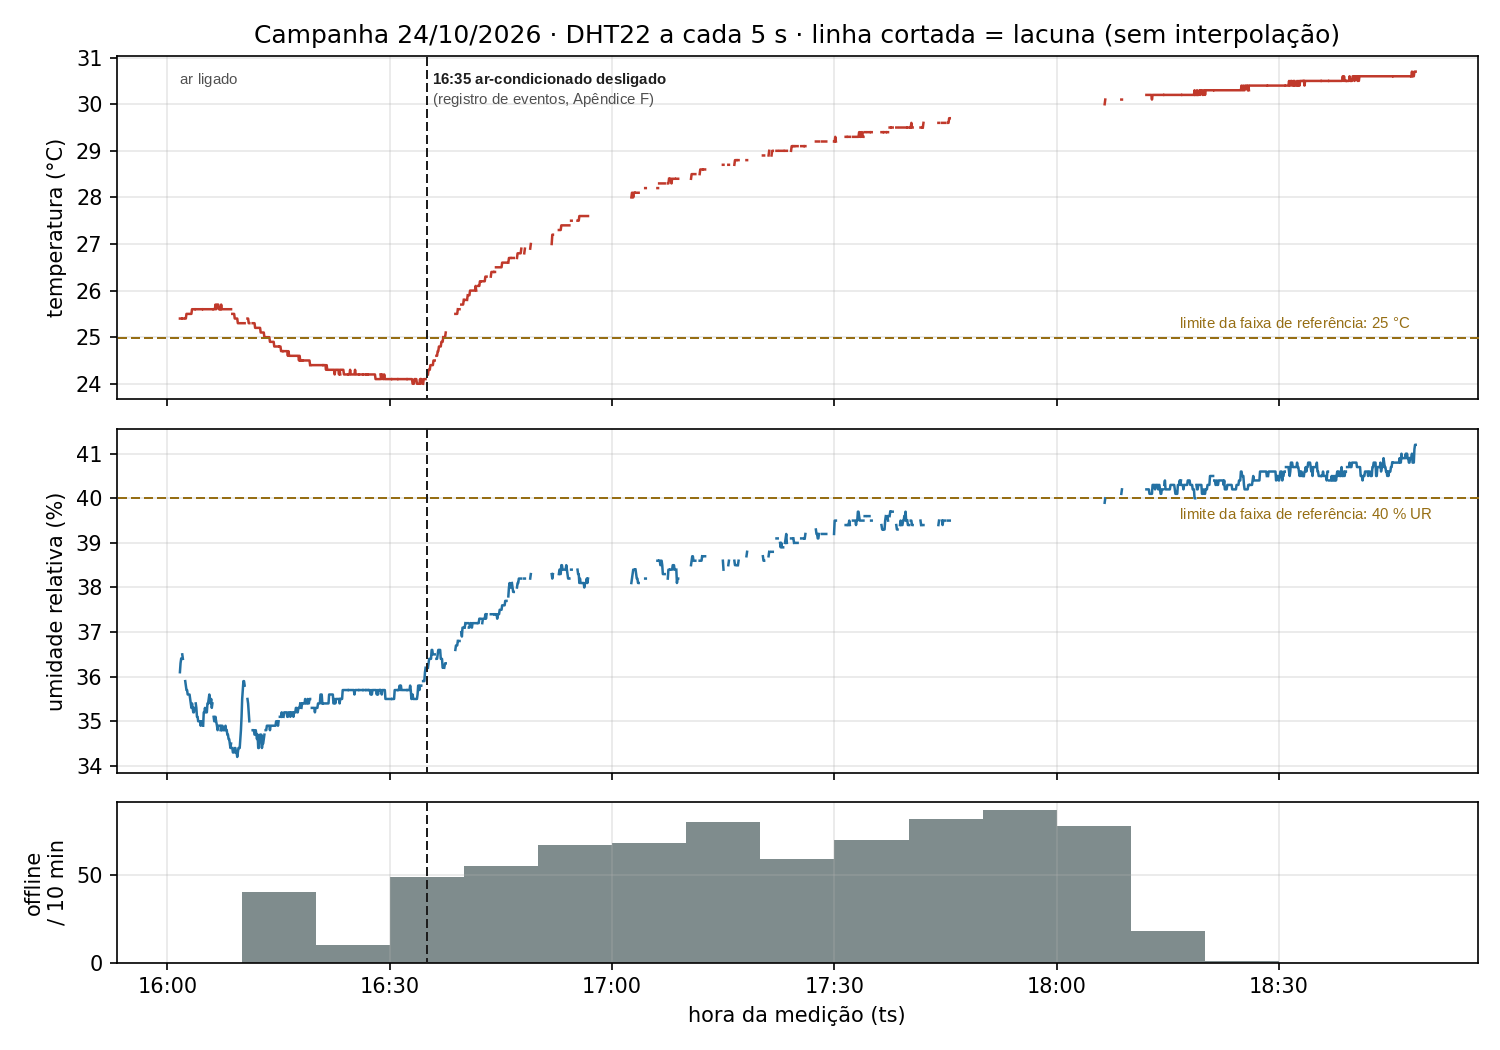
\includegraphics[width=0.95\textwidth]{figuras/serie-campanha-anotada.png}
\caption{Série temporal da campanha de coleta: temperatura, umidade
  relativa e quedas de conexão (\texttt{offline} a cada
  \SI{10}{\minute}), com o evento do registro (16:35) e os limites da
  faixa de referência. A linha é cortada onde falta leitura; nada foi
  interpolado}
\label{fig:resultado}
\fonte{Dados coletados pela equipe em 24/10/2026, das 16:01 às 18:48
  (\texttt{dados/campanha\_24-10-26/mensagens.csv}, branch
  \texttt{lab3}); gráfico gerado por \texttt{gravador/grafico.py}. As
  barras de \texttt{offline} usam a hora de chegada ao gravador; a de
  16:10 inclui os testamentos de 16:01 a 16:10, que chegaram no lote
  guardado pelo \emph{broker}. A linha do evento e as da faixa de
  referência foram acrescentadas pela equipe sobre a saída do
  \texttt{grafico.py}, que está sem anotações em
  \texttt{dados/campanha\_24-10-26/serie\_temporal.png}.}
\end{figure}

A série mostra um único evento, e ele está anotado: o ar-condicionado
do cômodo foi desligado às 16:35 (Apêndice~\ref{ap:campanha}). Com o ar
ligado, a temperatura caiu devagar, de 25,7 para \SI{24,0}{\celsius}.
Desligado o aparelho, ela subiu cerca de \SI{2}{\celsius} em
\SI{6}{\minute} (\SI{24,0}{\celsius} pouco antes, \SI{24,2}{\celsius} às
16:35 e \SI{26,0}{\celsius} às 16:41) e
continuou subindo, cada vez mais devagar, até \SI{30,7}{\celsius} no
fim, sem estabilizar. A curva é contínua mesmo durante a fase degradada
da conexão: as lacunas tiram pontos da série, mas não mudam a forma
dela. A umidade relativa subiu junto, de 34 para 41\,\%. Só o
aquecimento faria a umidade relativa cair; uma explicação compatível é
que o ar-condicionado, ligado, condensa e retira vapor do ar, e
desligado deixa de retirar. É uma hipótese: a umidade absoluta não foi
medida.

O alarme não aparece no gráfico porque o \emph{firmware} da campanha não
tem alarme (Seção~\ref{sec:firmware-com}). Aplicada depois, sobre o CSV,
a faixa padrão do \emph{firmware} da AP1 (a da sala de manipulação: 15
a \SI{25}{\celsius} e 40 a 70\,\% UR, Tabela~\ref{tab:config}) mostra
que o cômodo \textbf{nunca esteve dentro dela}: a temperatura só ficou
abaixo de \SI{25}{\celsius} entre 16:13 e 16:37, com o ar ligado, e ficou
acima dela em todas as 821 leituras depois das 16:37 (944 das \num{1213}
leituras com o DHT22, no total); a umidade ficou abaixo de 40\,\% UR até as 18:06 (778
leituras). Com a regra da Listagem~\ref{lst:alarme}, o nó da AP1 teria
pulsado o alarme a cada minuto durante toda a tarde. Não é defeito do
cômodo: a faixa é a de uma sala controlada, e um quarto em Teresina, de
tarde, não é uma; por isso a faixa é configurável por ambiente
(\RF{02}).

As lacunas estão na Tabela~\ref{tab:lacunas} e na barra de baixo da
Figura~\ref{fig:resultado}. Todas coincidem com quedas de conexão
registradas no \texttt{status}: o nó não reiniciou sozinho, o gravador
não parou, e não houve falta de energia. A maior parte delas está entre
16:30 e 18:10, a fase em que o nó conectava e caía em ciclo
(Seção~\ref{sec:qualidade}).

\section{Requisitos atendidos}

\begin{orientacao}
Retome a Tabela~\ref{tab:rastreabilidade} e feche o placar: quantos
requisitos foram atendidos, quantos parcialmente, quantos não. Para cada
não atendido, uma frase dizendo o que faltou. Equipe que declara
honestamente dois requisitos não atendidos sai melhor do que equipe que
declara todos atendidos e é desmentida na demonstração.
\end{orientacao}

\textbf{Ponto de partida (AP1).} Dos 9 requisitos definidos no primeiro
ciclo, a AP1 declarou 2 atendidos (\RF{01} e \RNF{03}), 4 parciais
(\RF{02}, \RF{03}, \RF{04} e \RNF{01}) e 3 não verificados ou não
atendidos (\RNF{02}, com latência observada de $\approx$\SI{5}{\second}
contra a meta de \SI{2}{\second}; \RNF{04} e \RNF{05}, não testados). As
pendências eram: o ensaio de alteração de faixa (\RF{02}), a latência do
alarme (\RNF{02}), o log formal da cessação do alarme (\RF{04}), a
medição de autonomia com bateria real (\RNF{01}) e os ensaios de faixa de
operação e de interferência (\RNF{04} e \RNF{05}). O \RF{01} continua
atendido, agora com a conta explícita: o \CT{01} rodou em modo
acelerado, mas dele se deduz a parte ativa do ciclo ($\approx$\SI{8,7}{\second}),
e com o sono de \SI{600}{\second} o ciclo fica 1,5\,\% acima de
\SI{10}{\minute}, dentro da tolerância.

\textbf{Placar da AP2.} Com os 7 requisitos de comunicação e de dados
acrescentados neste ciclo (\RF{05} a \RF{08} e \RNF{06} a \RNF{08}), o
sistema tem 16 requisitos: \textbf{5 atendidos} (\RF{01}, \RF{05},
\RF{07}, \RNF{03} e \RNF{06}), \textbf{8 parciais} (\RF{02}, \RF{03},
\RF{04}, \RF{06}, \RF{08}, \RNF{01}, \RNF{05} e \RNF{08}) e \textbf{3
não atendidos ou não testados} (\RNF{02}, \RNF{04} e \RNF{07}). Dos
cinco atendidos, dois se apoiam em estimativa declarada: o \RF{01}
(intervalo extrapolado do \CT{01}) e o \RF{07} (atraso do testamento
descontado o trânsito até o gravador). Os que não foram atendidos:

\begin{itemize}
  \item \RNF{07}: a completude foi de 63,1\,\%, contra a meta de
    95\,\%. As fases estáveis ficaram em 96\,\%, no limite da meta; a
    fase degradada, de \SI{1}{\hour} e \SI{40}{\minute}, derrubou a
    média. Faltou fila local, que teria guardado as leituras das quedas
    curtas, e faltou confirmar a causa das quedas;
  \item \RNF{02} e \RNF{04}: continuam como na AP1. O \emph{firmware}
    da campanha não tem alarme, e nenhum dos dois foi refeito.
\end{itemize}

\noindent Os parciais ficaram assim por motivos concretos: o \RF{06}
reconecta sozinho (nas 553 quedas do \emph{broker} da campanha, em
\SI{3,5}{\second} na mediana e em até \SI{30}{\second} em 552 delas),
mas não guarda; o \RF{08} não tem o \texttt{boot}; o \RNF{08} foi verificado até
\SI{8,7}{\minute}, e não até os \SI{10}{\minute} da meta; o \RNF{01}
chega a $\approx$29 dias só com o nó central e LoRa (estimativa de
folha de dados, sem o módulo), e o nó que publica direto ao roteador
fica em 21 dias, o número que leva o produto a ter um nó central
(\DP{6} e \DP{8}). O \RNF{05} passou de \enquote{não testado} a parcial com os
33 minutos de ar-condicionado ligado da campanha. Das pendências da AP1,
nenhuma foi resolvida neste ciclo: o trabalho foi
para a comunicação, que rodou num \emph{firmware} separado.

\section{Discussão}

\begin{orientacao}
Cinco perguntas, uma resposta curta para cada. As três primeiras vêm da
AP1 e continuam valendo; as duas últimas são da AP2.
\end{orientacao}

\begin{enumerate}[label=\arabic*.]
  \item \textbf{O sistema responde à pergunta de projeto do
    Capítulo~\ref{cap:problema}?} Na AP1, a resposta cobria apenas a
    metade local da pergunta: captar temperatura e umidade e sinalizar
    no ambiente quando saem da faixa. Na AP2, as leituras passaram a
    chegar a um ponto central, o gravador, com \SI{0,8}{\second} de
    atraso mediano, e um nó morto aparece no \texttt{status} em
    \SI{46}{\second}. Levadas pela ponte ao servidor do produto, as
    \num{1213} leituras da campanha entraram no banco e no painel sem
    nenhuma rejeitada (\CT{16}): o caminho até o servidor central da
    pergunta de projeto foi exercitado de ponta a ponta com dado real,
    ainda sem o nó central em hardware. Mas as duas metades ainda não estão no mesmo nó: o
    \emph{firmware} que publica não tem o alarme, e o que tem o alarme
    não publica. E, numa tarde, 37\,\% das leituras não chegaram: a
    condição da sala passou a ser conhecida sem ronda nos trechos
    estáveis, e não durante a fase degradada.
  \item \textbf{Qual decisão de projeto se mostrou mais acertada, e qual
    a equipe refaria?} Na AP1, a equipe apontou o processamento dos dados
    agregados fora do nó (\DP{5}), pelo custo energético de qualquer
    processamento extra na borda, e não identificou decisão a refazer.
    Na AP2, a mais acertada foi guardar o dado num assinante com sessão
    persistente (\DP{7}): o gravador começou \SI{8,7}{\minute} atrasado e
    não perdeu nenhuma leitura por isso. A que a equipe refaria é
    publicar só quando há conexão, sem fila: foi ela que transformou cada
    queda de conexão em leitura perdida. O \emph{deep sleep} da \DP{4}
    não chegou à campanha: o nó ficou sempre conectado e na USB
    (\DP{6}).
  \item \textbf{Se a autonomia real for metade da calculada, o projeto
    ainda faz sentido?} Na AP1, a equipe respondeu que uma autonomia pela
    metade tornaria a manutenção mais frequente do que o modelo de
    negócio pretende, em ambientes de acesso restrito. Com o rádio
    medido, a autonomia calculada do nó que publica direto ao roteador é
    de 21 dias; a metade seria cerca de 10 dias, uma troca de bateria a
    cada semana e meia, o que não faz sentido para o produto. Por isso o
    produto passa a ter um nó central (\DP{6} e \DP{8}): com LoRa, o
    rádio do nó de borda deve custar 2 a \SI{3}{\mAh}/dia
    (\folhadedados), a autonomia fica em $\approx$29 dias, e a metade
    dela, perto dos 15 dias, ainda é o dobro da do WiFi direto. O número
    só será confirmado quando o módulo LoRa chegar.
  \item \textbf{A tecnologia escolhida se sustentou?} O WiFi, sim: com
    RSSI entre \SI{-15}{} e \SI{-29}{dBm}, o enlace de rádio não foi o
    problema. O que não se sustentou foi a conexão MQTT ao \emph{broker}
    público: 764 quedas em \SI{2,78}{\hour} e completude de 63,1\,\%,
    contra cerca de 96\,\% nos trechos estáveis. O WiFi deixaria de
    servir com o nó a mais de duas paredes ou \SI{11}{\metre} do
    roteador, ou dentro de uma câmara metálica (\DP{8}).
  \item \textbf{O conjunto de dados responde ao que a equipe quer fazer
    na AP3?} Ainda não. Ele tem um único exemplo do evento de interesse,
    o ar-condicionado desligado às 16:35, numa só tarde, num cômodo e
    não no cenário de referência. Serve para escolher a janela e as
    características (a taxa de subida da temperatura e a umidade
    subindo junto); para treinar e validar, faltam mais eventos
    anotados (Seção~\ref{sec:dataset}).
\end{enumerate}

% =====================================================================
%  Capítulo 9 — Limitações e próximo ciclo
% =====================================================================
\chapter{Limitações e próximo ciclo}
\label{cap:conclusao}
\rubricaComunicacao

\begin{orientacao}
Uma página. Sem repetir o resumo e sem adjetivo de autoelogio.
\end{orientacao}

\section{Limitações conhecidas}

\begin{orientacao}
O que o sistema não faz, o que só funciona sob condições controladas e
qual número do relatório é o mais frágil. Todo projeto deste ciclo tem
pelo menos um número que é estimativa: identifique-o. As limitações
abaixo vêm da AP1; mantenham só as que continuam valendo e acrescentem
as da AP2.
\end{orientacao}

\textbf{Herdadas da AP1, e que continuam valendo.} A autonomia da
\RNF{01} continua calculada, e não medida: os 21 dias de agora usam o
tempo de rádio medido, mas nenhum ensaio com bateria real foi feito, e o
consumo do alarme segue fora da conta. A robustez a interferência
eletromagnética (\RNF{05}) ganhou só uma evidência indireta, os 33
minutos de ar-condicionado ligado na campanha, sem o ensaio dedicado
junto a um compressor. A lógica de mudança de faixa (\RF{02}) continua
falhando nos testes de bancada da AP1, a cessação do alarme (\RF{04})
continua sem log formal, e o sensor desconectado ainda leva o nó a um
laço de reinícios pelo \emph{watchdog} (\CT{05}). Nenhuma delas foi
tratada neste ciclo.

\textbf{Da AP2.} A campanha durou \SI{2,78}{\hour}, numa tarde de
24/10, num cômodo com ar-condicionado e não no cenário de referência, com
um nó na USB e o roteador no mesmo ambiente; ela não mostra o ciclo
diário, a madrugada, as paredes da farmácia nem a porta do freezer. As
demais limitações conhecidas:

\begin{itemize}
  \item \textbf{O nó que publica não é o nó que alarma.} O
    \emph{firmware} da campanha (branch \texttt{lab3}) não tem a leitura
    filtrada, o alarme local, a configuração na NVS nem o \emph{deep
    sleep} da AP1; o \emph{firmware} da AP1 não publica. Tudo o que o
    Cap.~\ref{cap:testes} mede de comunicação vale para o primeiro, e
    tudo o que mede de alarme, para o segundo.
  \item \textbf{Sem fila local e sem \texttt{boot}.} Toda queda de
    conexão vira leitura perdida de vez (cerca de 740 na campanha), e um
    reinício só é reconhecido se a primeira leitura depois dele chegar.
  \item \textbf{A causa da fase degradada é uma hipótese.} O
    \emph{timeout} de \SI{1}{\second} da biblioteca MQTT explica o padrão
    das quedas, mas a latência até o \emph{broker} não foi medida e o
    teste com \emph{timeout} maior não foi feito. O número mais frágil
    da AP2, depois da corrente do rádio, é a própria completude: outra
    tarde, com outra carga na rede, poderia dar 96\,\% ou menos que
    63\,\%.
  \item \textbf{\emph{Broker} público, sem autenticação.} Qualquer
    pessoa poderia ter publicado em \texttt{ufpi-iot26/eq01/\#}; nada
    estranho chegou, mas nada impedia.
  \item \textbf{Período de \SI{5}{\second}, e não de \SI{600}{\second}.}
    A campanha não exercita o período do \RF{01} nem mede a energia do
    nó sempre conectado.
  \item \textbf{O número mais frágil é a corrente do rádio.} Os
    \SI{300}{\milli\ampere} da Seção~\ref{sec:custo-radio} são da placa
    inteira, lidos no medidor USB, e não do ESP32; com a estimativa
    anterior de \SI{120}{\milli\ampere}, a autonomia calculada passaria de
    21 para 26 dias. O tempo de rádio, ao contrário, foi medido com
    \texttt{millis()} em 36 ciclos.
  \item \textbf{A conexão TLS foi medida contra um servidor de eco, não
    contra o \emph{broker} da campanha}, e a corrente do nó conectado e
    ocioso, que é o que pesa num nó que não dorme (\DP{6}), não foi
    medida.
  \item \textbf{O alcance foi medido num ambiente interno de teste, com
    um único teste de \SI{60}{\second} por posição}, sem caracterizar as
    paredes nem controlar a orientação das placas; a contagem de paredes
    digitada a 8 e \SI{11}{\metre} difere entre as baterias de ESP-NOW e
    de BLE, embora o RSSI mostre que as posições foram as mesmas
    (Apêndice~\ref{ap:testes}, \CT{15}).
    Câmaras frias e freezers, cujas paredes metálicas devem atenuar muito
    mais, não foram testados.
  \item \textbf{Os testes de robustez da AP1 (\CT{05} e \CT{06}) foram
    feitos com um DHT11}, e não com o DHT22 do projeto; o comportamento
    observado (laço de reinícios e recuperação da NVS) não depende do
    sensor, mas a precisão declarada nas mensagens, sim.
  \item \textbf{O nó não confere o certificado do \emph{broker}}
    (\texttt{setInsecure()}, herdado do Lab~03): a conexão é cifrada, mas
    não autenticada.
  \item \textbf{LoRa/LoRaWAN, a tecnologia escolhida para o produto, não
    foi testado}: o módulo comprado pela equipe não chegou a tempo. O
    alcance, o tempo no ar e o consumo do LoRa vêm da matriz de 22/09, da
    folha de dados e da conta do ar da Aula~14, e não de medição; a
    autonomia de $\approx$29 dias do nó de borda é estimativa. Os
    substitutos testados no lugar dele foram medidos numa casa, e não na
    farmácia: o ESP-NOW foi bem até \SI{8}{\metre} com uma parede, mas
    pode não repetir esse resultado no nosso caso de uso, e o interior do
    freezer não foi testado com nenhum rádio. O nó central continua sem hardware
    definido.
\end{itemize}

\section{O que entra no próximo ciclo}

\begin{orientacao}
Ligue este relatório ao seguinte.
\aPartirDaAP{1}{}%
\seAP{1}{Na AP2 a equipe vai integrar este sistema a uma infraestrutura
de comunicação e formar o conjunto de dados do projeto: diga qual
tecnologia é a candidata e qual linha do orçamento de energia vai ser
medida em vez de estimada.}%
\seAP{2}{Na AP3 a equipe vai treinar e embarcar um modelo: diga o que
pretende classificar ou prever, e se o conjunto de dados formado neste
ciclo é suficiente para isso.}%
\seAP{3}{Diga o que o projeto precisaria para sair do laboratório e
virar algo instalado no contexto do Capítulo~\ref{cap:problema}:
alimentação, invólucro, manutenção, custo por unidade em escala.}
\end{orientacao}

Na AP3 a equipe vai treinar e embarcar um modelo sobre o conjunto de
dados formado neste ciclo. O que se pretende é detectar uma falha de
climatização --- o ar-condicionado que desliga, ou a porta de um
freezer que fica aberta --- pela forma da curva de temperatura e
umidade, antes que a leitura saia da faixa. O conjunto tem \textbf{um} exemplo desse evento, anotado no
registro do Apêndice~\ref{ap:campanha} (16:35 de 24/10), o que não
basta para treinar nem para validar. Falta coletar mais
desligamentos, em dias e horários diferentes e de preferência no
cenário de referência, e trechos longos sem evento.

Antes disso, o \emph{firmware} precisa de três mudanças, nesta ordem:
uma fila local, para que uma queda de conexão atrase a leitura em vez
de apagá-la; o \texttt{boot} no contrato; e a união com o
\emph{firmware} da AP1, para que o nó que publica seja o mesmo que
alarma. Junto com elas, o teste do \emph{timeout} da biblioteca MQTT
(\texttt{mqtt.setTimeout(5000)}) com a contagem de \texttt{offline}
antes e depois. Quando o módulo LoRa chegar, o enlace entre o nó de
borda e o nó central passa a ser LoRa, com o contrato em binário de 8
bytes, e o alcance e o consumo dele serão medidos nas mesmas posições
das baterias de ESP-NOW e BLE, de preferência também com o nó dentro de
um freezer.

A ponte com o servidor do produto (\CT{16}) resolveu duas questões do
contrato e deixou duas para o próximo ciclo. Resolvidas: a hora da
leitura continua sendo a do nó (o \texttt{ts} do NTP vira o
\texttt{data\_hora} em UTC), e o \texttt{lote\_id} derivado do nó e do
intervalo de \texttt{seq} torna o reenvio idempotente, como o reenvio dos
13 lotes mostrou. Abertas: no produto, o nó de borda em \emph{deep sleep}
com LoRa não terá NTP, e a hora terá de vir do nó central, com o
atraso declarado no contrato; e o \texttt{boot} precisa entrar no
\texttt{lote\_id}, para que um reinício não gere o mesmo identificador
para leituras diferentes. O servidor tem ainda um defeito a corrigir:
um lote com várias leituras fora da faixa em temperatura e umidade
derruba a abertura de alertas (HTTP 500), e o lote é recusado inteiro.

\section{Divisão do trabalho}

\begin{orientacao}
Uma linha por integrante, dizendo o que cada um fez neste ciclo. Os
papéis rotacionam a cada módulo: ninguém repete na AP2 o papel que teve
na AP1. Na AP1: João Pedro na integração; Victor e Davi no
\emph{firmware}; Felipe no \emph{hardware} e nos testes; Luanderson na
documentação.
\end{orientacao}

Os papéis rotacionaram em relação à AP1, e cada integrante ficou com
uma frente. Os \emph{commits} da AP2 foram enviados ao repositório por
um único integrante (João Pedro), que concentrou a inserção do material
de todos; por isso a autoria das tarefas é a desta lista, e não a do
histórico do Git.

\begin{itemize}
  \item \textbf{Felipe} (\emph{firmware} e comunicação; na AP1,
    \emph{hardware} e testes): \emph{firmware} MQTT da campanha sobre o
    sketch do Lab~03 (DHT22 no \texttt{GPIO4}, tópicos da equipe, NTP,
    testamento e sessão persistente); \emph{firmware} de sensor e de
    \emph{gateway} das baterias de ESP-NOW e de BLE; ferramenta da
    Aula~10 que cronometra o ciclo de rádio (branches \texttt{lab3},
    \texttt{teste-esp-now}, \texttt{teste-ble} e
    \texttt{apendice\_b}).
  \item \textbf{João Pedro} (dados --- gravador e qualidade; na AP1,
    integração): mudanças no \texttt{gravador.py} e no
    \texttt{qualidade.py}, \texttt{grafico.py} novo, gravadores seriais
    das baterias e reanálise dos dados brutos (\texttt{analise.py});
    hospedou os testes de falha e a campanha, com o nó, o roteador e o
    notebook do gravador, e anotou os eventos do ambiente.
  \item \textbf{Luanderson} (dados --- campanha e registro de eventos;
    na AP1, documentação): roteiro dos testes de falha e da campanha,
    ficha da campanha, diário e registro de eventos
    (Apêndice~\ref{ap:campanha}), contagens sobre o CSV (fases, quedas de
    conexão, atraso) e consolidação dos números usados no relatório.
  \item \textbf{Victor} (integração --- repositório, \emph{broker} e
    serviços de telemetria; na AP1, \emph{firmware}): organização do
    repositório e das branches de trabalho, \emph{commit} da entrega com
    a \emph{tag} \texttt{ap2}, contrato de tópicos e configuração do
    \emph{broker}, e a ligação com o servidor do produto (nó central,
    lote e chave de API).
  \item \textbf{Davi} (documentação --- relatório, registro de decisões e
    prazos; na AP1, \emph{firmware}): migração do relatório para o modelo
    da AP2, caixas de decisão do Módulo~2 (\DP{6} a \DP{8}), tabela de
    rastreabilidade, declaração de IA e controle dos prazos da entrega.
\end{itemize}

\imprimirTabelaIntegrantes


% ---------- ELEMENTOS PÓS-TEXTUAIS -----------------------------------
\postextual

% As referências são citadas no texto (Caps. 3 e 5); não há mais \nocite.
\bibliography{referencias}

\begin{apendicesenv}
  \partapendices
  % =====================================================================
%  Apêndice A — Mapa de barramento
%  Instrumento da Aula 06 (31/08), entregue em 01/09.
% =====================================================================
\chapter{Mapa de barramento}
\label{ap:barramento}

\begin{orientacao}
Transcreva aqui o mapa entregue em 01/09, \textbf{atualizado} para os
componentes que de fato estão no protótipo. Uma linha por dispositivo.
Se algum componente ainda não chegou, mantenha a linha e marque
\emph{(previsto)}.
\end{orientacao}

\begin{table}[H]
\centering
\caption{Mapa de barramento do protótipo}
\label{tab:barramento}
\scriptsize
\setlength{\tabcolsep}{3.5pt}
\begin{tabular}{@{}L{2.4cm}L{3.0cm}L{1.5cm}L{2.5cm}L{2.4cm}C{1.0cm}C{1.6cm}@{}}
\toprule
\textbf{Dispositivo} & \textbf{O que mede ou faz} & \textbf{Barra\-mento}
& \textbf{Como é selecionado} & \textbf{Pinos na D1 R32} & \textbf{Ten\-são}
& \textbf{Leituras por segundo} \\
\midrule
DHT22 / AM2302 & Temperatura e umidade relativa & digital 1 fio (proprietário) & ponto a ponto (protocolo próprio, não endereçável) & DATA: GPIO4 (A1), pull-up 10\,k$\Omega$ até 3V3 & 3V3 & 1 a cada 600\,s (\RF{01}); internamente, até 1 a cada 2,1\,s durante a amostragem \\
LED de status & Indica nó acordado (bancada) & GPIO digital & saída dedicada, sem endereço & GPIO25 (D3) & 3V3 & aceso durante todo o ciclo acordado ($\approx$\SI{12}{\second}) \\
Divisor de \texttt{VBAT} (opcional) & Tensão da bateria & ADC (analógico) & ADC1 dedicado, sem endereço & GPIO34 (A2), só entrada & 0--\SI{2.1}{\volt} na entrada do ADC & 1 por ciclo de leitura (600\,s) \\
UART0 & Upload de firmware e monitor serial & UART & ponto a ponto & GPIO1 / GPIO3 (D0 / D1) --- \textbf{reservado, não ocupar} & 3V3 & sob demanda (bancada) \\
Buzzer ativo (alarme) & Sinalização sonora de desvio & GPIO digital & saída dedicada, sem endereço & GPIO26 (D4), acionado em nível alto & 3V3 & sob evento: pulso de \SI{3}{\second} a cada \SI{60}{\second} fora da faixa (\RF{03}) \\
LED de alarme & Sinalização visual de desvio & GPIO digital & saída dedicada, sem endereço & GPIO27 (D5), resistor de $\approx$\SI{330}{\ohm} & 3V3 & junto com o buzzer (\RF{03}) \\
\bottomrule
\end{tabular}
\fonte{Elaborada pela equipe, com base no firmware \texttt{esp32\_dht22.ino} e seu README. O \emph{firmware} de comunicação da campanha usa só o DHT22 no mesmo GPIO4, lido uma vez a cada \SI{5}{\second}, e o rádio WiFi interno.}
\end{table}

\begin{orientacao}
Lembretes das colunas, na ordem: o \textbf{barramento} é
I\textsuperscript{2}C, SPI, 1-Wire, UART ou analógico (ADC);
\textbf{como é selecionado} responde \emph{como o mestre diz
\enquote{você, agora}} --- endereço (\texttt{0x76}), pino de CS
(\texttt{GPIO5}), ROM ID ou \enquote{ponto a ponto} para UART;
\textbf{pinos} exige a serigrafia \emph{e} o GPIO
(\texttt{SDA/SCL (21/22)}); e \textbf{leituras por segundo} é o que a
\emph{aplicação} exige, não o máximo que o sensor entrega.
\end{orientacao}

\section*{Decisões de barramento}
\phantomsection
\addcontentsline{toc}{section}{Decisões de barramento}

\begin{description}[style=unboxed, leftmargin=0pt, font=\normalfont\bfseries]
  \item[1. Conflitos de pino encontrados, e como foram resolvidos.]\hfill\\
    Nenhum conflito de pino ocupado. A equipe descartou de antemão os
    pinos \texttt{GPIO2} (LED\_BUILTIN + \emph{strapping} de boot) e
    \texttt{GPIO12} (\emph{strapping} ligado à tensão da flash), e os
    pinos \texttt{A2}--\texttt{A5}, que são só entrada e por isso não
    servem ao dado do DHT22, que precisa também escrever.
  \item[2. Colisões de endereço, se há dois dispositivos I\textsuperscript{2}C iguais.]\hfill\\
    Não se aplica: o DHT22 não usa I\textsuperscript{2}C, e sim um
    protocolo próprio ponto a ponto, sem endereço configurável. Cada
    DHT22 adicional exigiria um pino de dado dedicado --- não há como
    endereçar dois no mesmo fio.
  \item[3. O dispositivo mais lento do conjunto, e quanto ele custa ao laço.]\hfill\\
    O próprio DHT22, que exige um intervalo mínimo de \SI{2}{\second}
    entre leituras (limite do fabricante, não escolha do projeto). O
    \emph{firmware} absorve esse custo porque o ciclo inteiro já é
    dedicado à leitura --- entre um despertar e o próximo, o nó está
    em \emph{deep sleep}, então não há outra tarefa concorrente para
    essa espera atrapalhar.
  \item[4. O que mudou com o rádio (AP2).]\hfill\\
    Com o WiFi ligado, o ADC2 do ESP32 deixa de ser confiável; o
    divisor de \texttt{VBAT} já estava no \texttt{GPIO34}, do ADC1, e
    não precisou mudar. A espera do DHT22 passou a importar: no
    \emph{firmware} de comunicação há uma tarefa concorrente, o
    \texttt{mqtt.loop()}, que não pode ficar mais de $1{,}5 \times$ o
    \emph{keepalive} (\SI{45}{\second}) sem rodar. A leitura única de
    agora não pesa; a mediana de 5 amostras da AP1 seguraria o laço por
    cerca de \SI{8,4}{\second}, o que ainda cabe
    (Seção~\ref{sec:firmware-com}).
\end{description}

  % =====================================================================
%  Apêndice B — Orçamento de energia
%  Instrumento da Aula 08 (09/09), entregue em 13/09.
% =====================================================================
\chapter{Orçamento de energia}
\label{ap:energia}

\begin{orientacao}
Uma linha por \textbf{estado} do sistema, e os estados têm de cobrir as
24 horas do dia. Os estados desta tabela precisam ser os mesmos da
máquina de estados da Seção~\ref{sec:firmware}. A conta de cada linha é
\[
  \text{carga}\,[\si{\mAh}/\text{dia}] =
  \frac{\text{corrente}\,[\si{\milli\ampere}] \times
        \text{duração}\,[\si{\second}] \times \text{ciclos/dia}}{3600}.
\]
\end{orientacao}

\begin{orientacao}
Na AP2, a linha do rádio deixa de ser estimativa: entram os números
medidos da Seção~\ref{sec:custo-radio}, e a autonomia é recalculada.
Se o nó deixou de usar \emph{deep sleep} para manter a conexão com o
\emph{broker}, os estados desta tabela mudam junto com a máquina de
estados da Seção~\ref{sec:firmware}.
\end{orientacao}

\begin{table}[H]
\centering
\caption{Orçamento de energia do protótipo}
\label{tab:energia}
\scriptsize
\setlength{\tabcolsep}{3.5pt}
\begin{tabular}{@{}L{2.6cm}L{3.0cm}R{1.5cm}R{1.7cm}R{1.3cm}R{1.6cm}L{2.4cm}@{}}
\toprule
\textbf{Estado} & \textbf{O que está ligado} & \textbf{Corrente (mA)}
& \textbf{Duração por ciclo (s)} & \textbf{Ciclos /dia}
& \textbf{Carga (mA$\cdot$h /dia)} & \textbf{Origem do número} \\
\midrule
acorda e lê     & ESP32 ativo + DHT22 em leitura & 46,5 & 12,0 & 144 & 22,32 & \folhadedados \\
transmite (AP2) & rádio WiFi: associa, DHCP, DNS, conecta, publica e desliga (pior de 10 ciclos HTTP; na AP1, \enquote{não se aplica}) & 300,0 & 2,48 & 144 & 29,70 & \bancada{} (tempo, \texttt{millis()}) + \bancada{} (corrente, medidor USB na rajada de 23/10) \\
aciona o atuador& buzzer + LED de alarme: pulso de \SI{3}{\second} em cada ciclo fora da faixa, que passa a ser de \SI{60}{\second} & 35,0 & 3,0 & depende do tempo fora da faixa & --- & \estimativa{} (corrente); \emph{firmware} (duração) \\
dorme           & ESP32 em deep sleep & 2,0 & 588,0 (AP1) 585,52 (AP2) & 144 & 47,04 (AP1) 46,84 (AP2) & \bancada \\
\midrule
\multicolumn{5}{@{}r}{\textbf{Total diário na AP1 (sem rádio e sem o alarme)}} & \textbf{69,4} & \\
\multicolumn{5}{@{}r}{\textbf{Total diário na AP2 (com o rádio medido, sem o alarme)}} & \textbf{98,9} & \\
\bottomrule
\end{tabular}
\fonte{Elaborada pela equipe, com base nas constantes do firmware \texttt{esp32\_dht22.ino} (ajustadas para o ciclo de 10 min do \RF{01}) e na medição de 23/10 (branch \texttt{apendice\_b}, \texttt{gravador/dados/resumo.md}). Na versão da AP1 desta tabela, a coluna de carga trazia 0,22 e 0,47, os valores divididos por 100; o total de 69,4 já estava certo.}
\end{table}

\begin{orientacao}
\textbf{Estimativa é resposta legítima, desde que declarada.} Número sem
procedência não é número. Use \verb|\folhadedados|, \verb|\bancada| ou
\verb|\estimativa| na última coluna.
\end{orientacao}

\section*{Quatro linhas de decisão}
\phantomsection
\addcontentsline{toc}{section}{Quatro linhas de decisão}

\begin{description}[style=unboxed, leftmargin=0pt, font=\normalfont\bfseries]
  \item[1. Consumo diário total e consumo médio.]\hfill\\
    Aproximadamente \SI{69.4}{\mAh}/dia na AP1 (excluindo o alarme), o
    que equivale a uma corrente média de $69{,}4/24 \approx
    \SI{2.9}{\milli\ampere}$. \textbf{Na AP2}, com o ciclo de rádio
    medido, \SI{98.9}{\mAh}/dia, ou \SI{4.12}{\milli\ampere} de média. O
    alarme continua fora da conta: sua corrente segue sem medição.
  \item[2. Fonte de alimentação escolhida, e por quê.]\hfill\\
    Bateria recarregável (Li-ion 18650), porque os pontos de instalação
    mais exigentes --- dentro de um freezer ou próximos a uma câmara
    fria --- nem sempre têm tomada acessível, e a fiação até a rede
    elétrica é uma das restrições já registradas no
    Capítulo~\ref{cap:requisitos}.
  \item[3. Autonomia estimada, e a conta que levou até ela.]\hfill\\
    Com uma 18650 de \SI{2600}{\mAh} e 80\,\% de profundidade de
    descarga útil, a capacidade útil é de $2600 \times 0{,}80 =
    \SI{2080}{\mAh}$. Autonomia $= 2080 / 69{,}4 \approx$ \textbf{30
    dias}. Este número cobre apenas o sensoriamento; será revisto para
    baixo assim que o consumo do alarme for medido e somado.

    \textbf{Na AP2}, com o rádio medido: autonomia $= 2080 / 98{,}9
    \approx$ \textbf{21 dias}. Com TLS, usando a mediana do ciclo HTTPS
    (\SI{3,16}{\second}), $2080 / 107{,}0 \approx 19$ dias; com a
    estimativa antiga de \SI{120}{\milli\ampere} para o rádio, seriam
    $2080 / 81{,}0 \approx 26$ dias. Na arquitetura proposta para o
    produto (\DP{6}~(c)), o nó de borda não associa ao roteador: manda
    a leitura por LoRa ao nó central, a 2 a \SI{3}{\mAh}/dia
    (\folhadedados, matriz de 22/09), e a conta fica em
    $2080 / 71{,}4 \approx 29{,}1$ a $2080 / 72{,}4 \approx 28{,}7$
    dias, \textbf{$\approx$29 dias}, perto do alvo do \RNF{01}. A linha
    do LoRa só será medida quando o módulo chegar.
    Nenhum desses números foi verificado com bateria real (\CT{07}).
  \item[4. O que acontece quando a energia acaba --- ou enquanto o nó dorme.]\hfill\\
    Enquanto dorme, o nó está em estado seguro por definição: não há
    atuador acionado durante o \emph{deep sleep}, e a próxima leitura
    ocorre no horário programado pelo temporizador. Quando a bateria se
    esgota, o nó simplesmente para de acordar --- e, como não havia rede
    na AP1, \textbf{nada nem ninguém era avisado disso}. Na AP2, com o
    nó conectado ao \emph{broker}, o testamento publica \texttt{offline}
    em até \SI{45}{\second} depois da última notícia do nó, e o gravador
    registra a hora no CSV (na campanha, \SI{46}{\second}, \CT{10});
    ninguém recebe um aviso automático, e as quedas só são vistas por
    quem abre o terminal do gravador ou o MQTT Explorer. Num nó que dorme entre leituras (opção (a) da
    \DP{6}), o testamento não serve para isso, porque o nó sai do
    \emph{broker} a cada ciclo; quem denuncia o nó morto é a falta de
    leituras.
\end{description}

\section*{Se a conta atravessar tensões diferentes}
\phantomsection
\addcontentsline{toc}{section}{Se a conta atravessar tensões diferentes}

\begin{orientacao}
\SI{}{\mAh} só se somam dentro do mesmo barramento de tensão. Se algum
atuador funciona em outra tensão, converta para watt-hora antes de somar.
Use eficiência de 0,85 se não souber a do seu conversor.
\end{orientacao}

\begin{align*}
  E\,[\si{\Wh}] &= V\,[\si{\volt}] \times I\,[\si{\ampere}] \times t\,[\si{\hour}] \\[2pt]
  \text{carga na bateria}\,[\si{\mAh}] &=
    \frac{E\,[\si{\Wh}]}{\eta_{\text{conversor}} \times V_{\text{bateria}}\,[\si{\volt}]}
    \times 1000
\end{align*}

\section*{Se o projeto for alimentado por painel}
\phantomsection
\addcontentsline{toc}{section}{Se o projeto for alimentado por painel}

\begin{align*}
  E_{\text{diária}}\,[\si{\Wh}] &=
    \frac{\text{consumo}\,[\si{\mAh}]}{1000} \times V_{\text{bateria}}\,[\si{\volt}] \\[2pt]
  P_{\text{painel}}\,[\si{\watt}] &=
    \frac{E_{\text{diária}}}{\text{HSP} \times f_{\text{perdas}}} \times f_{\text{segurança}}
\end{align*}

\begin{orientacao}
Para Teresina, use a HSP do \textbf{pior mês} (Atlas Brasileiro de
Energia Solar ou SunData do CRESESB); a média anual fica perto de
\SI{5.5}{\kilo\watt\hour\per\square\metre} por dia, mas é o pior mês que
decide. Fator de perdas 0,6 e fator de segurança entre 2 e 3 são
conservadores e suficientes para esta disciplina. A bateria, nesse caso,
é dimensionada pelos \textbf{dias sem sol} que o projeto precisa
aguentar, não pelo consumo de um dia.
\end{orientacao}

\section*{Quem está dimensionando este sistema}
\phantomsection
\addcontentsline{toc}{section}{Quem está dimensionando este sistema}

\begin{orientacao}
Uma frase: qual estado responde pela maior fatia do consumo, e em que
percentual. Se a resposta for o atuador, a decisão que importa no
projeto não é de \emph{firmware}.
\end{orientacao}

O \emph{deep sleep} responde por cerca de 68\,\% do consumo diário
estimado da AP1 (\SI{47.0}{\mAh} dos \SI{69.4}{\mAh}/dia), mesmo sendo o
estado de menor corrente instantânea --- ele simplesmente dura muito
mais tempo que a leitura. Quem dimensiona este sistema, portanto, não
é o DHT22: é a corrente de repouso da placa em \emph{deep sleep}, o
que só poderá ser confirmado (e revisto) quando o consumo do alarme
for medido em bancada e somado a este orçamento.

\textbf{Na AP2}, com o rádio na conta, quem dimensiona o sistema
continua sendo o \emph{deep sleep}, mas agora com 47\,\% do consumo
diário (\SI{46.8}{\mAh} dos \SI{98.9}{\mAh}), seguido de perto pelo rádio,
com 30\,\%. Dentro do ciclo de rádio, quem pesa é o DHCP
(\SI{1,52}{\second} dos \SI{2,27}{\second}). A bateria de ESP-NOW de 24/10,
feita no lugar do LoRa, mostra o outro lado: com um módulo sem regulador
nem conversor USB (sono de \SI{65}{\micro\ampere}), o sono deixa de pesar,
e quem dimensiona passa a ser o rádio no pior enlace, com 82\,\% do
consumo a \SI{18}{\metre} (no modelo daquela bateria, com envio a cada
\SI{5}{\minute}). Num enlace ruim, as retransmissões custam mais que a
bateria economiza; é mais um motivo para o produto usar um rádio que
alcance o nó central com folga, como o LoRa.

  % =====================================================================
%  Apêndice C — Plano de testes
% =====================================================================
\chapter{Plano de testes}
\label{ap:testes}

\begin{orientacao}
Um quadro por caso de teste. O procedimento precisa ser executável por
alguém que não montou o sistema: se um passo diz \enquote{configurar o
sensor}, ele não é um passo. Copie o quadro abaixo quantas vezes forem
necessárias.
\end{orientacao}

\begin{table}[H]
\centering
\caption{CT-01 --- taxa de amostragem}
\label{tab:ct01}
\footnotesize
\setlength{\tabcolsep}{3.5pt}
\begin{tabular}{@{}L{3.2cm}L{12.0cm}@{}}
\toprule
\textbf{Requisito verificado} & \RF{01} \\
\midrule
\textbf{Objetivo} & Verificar que o intervalo entre amostras consecutivas
  fica dentro de $\pm$ 10\,\% do valor especificado. \\
\textbf{Material} & Protótipo montado, cabo USB, monitor serial a
  \SI{115200}{\baud}. \\
\textbf{Procedimento} &
  1. Gravar o \emph{firmware} da AP1 (\texttt{esp32\_dht22.ino}, branch
     \texttt{victor\#sensores}, Seção~\ref{sec:repositorio}).\newline
  2. Abrir o monitor serial e registrar \SI{100}{} linhas em arquivo.\newline
  3. Calcular a diferença entre carimbos de tempo consecutivos.\newline
  4. Comparar média e desvio com o valor especificado. \\
\textbf{Resultado esperado} & Média dentro de $\pm$ 10\,\%; nenhuma
  amostra com atraso superior ao dobro do período. \\
\textbf{Resultado obtido} & Ensaio executado com \texttt{TESTE\_100\_CICLOS=1}
  (sono reduzido a \SI{1}{\second} por ciclo, mediana de 5 amostras
  mantida). A primeira captura do log chegou corrompida e foi refeita; o
  arquivo recapturado ficou legível e mostra 99 dos 100 despertares com
  leitura completa (ciclo~1 fora da janela de captura), em sequência
  contínua de \#2 a \#100, sem nenhum travamento ou \emph{reboot}
  inesperado. O intervalo médio entre despertares consecutivos foi de
  \SI{9,7}{\second} (\SI{961}{\second} entre o primeiro e o último
  registro, divididos por 99 ciclos) --- acima do \SI{1}{\second} de sono
  configurado, pois o tempo ativo de leitura das 5 amostras, cálculo da
  mediana/EMA e impressão no serial também entra no ciclo. O tempo ativo
  não foi cronometrado à parte: os $\approx$\SI{8,7}{\second} saem da
  diferença entre o ciclo médio (\SI{9,7}{\second}) e o sono configurado
  (\SI{1}{\second}), supondo que o sono dure o que o \emph{firmware}
  programa. Temperatura (mediana) entre
  \SI{36,0}{\celsius} e \SI{36,8}{\celsius}, umidade entre
  \SI{20}{\percent} e \SI{34}{\percent}RH --- variação estreita, coerente
  com o sensor parado em bancada durante o ensaio; tensão de bateria
  \SI{0.00}{\volt} em 100\,\% dos registros (divisor de VBAT não montado
  neste ensaio, comportamento esperado). \\
\textbf{Veredito} & \aprovado{} (estimado: a parte ativa de $\approx$\SI{8,7}{\second} deduzida deste ensaio, somada ao sono de \SI{600}{\second} que o \emph{firmware} programa por inteiro, dá $\approx$\SI{608,7}{\second} por ciclo, +1,5\,\%, dentro dos $\pm$10\,\%) \\
\textbf{Evidência} & \texttt{teste\_100\_ciclos.log} (recapturado, legível).
  O veredito é \emph{estimado}, e não medido: o ensaio comprova
  estabilidade em 100 ciclos acelerados e a integridade dos dados
  registrados, mas não cronometra o sono separado do tempo ativo. A
  confirmação direta do intervalo de \SI{10}{\minute} do RF-01 depende de
  um ensaio em velocidade real (sem \texttt{TESTE\_100\_CICLOS}) ou de
  um \emph{log} com marcação separada de sono e processamento, que
  continua pendente (Seção~\ref{sec:oquefalhou}). \\
\bottomrule
\end{tabular}
\fonte{Elaborada pela equipe.}
\end{table}

\begin{table}[H]
\centering
\caption{CT-02 --- alteração da faixa de referência sem recompilar}
\label{tab:ct02}
\footnotesize
\setlength{\tabcolsep}{3.5pt}
\begin{tabular}{@{}L{3.2cm}L{12.0cm}@{}}
\toprule
\textbf{Requisito verificado} & \RF{02} \\
\textbf{Objetivo} & Verificar que os limiares de temperatura e umidade, e o
  intervalo entre leituras, podem ser alterados em tempo de execução, sem
  novo \emph{upload} de \emph{firmware}. \\
\textbf{Material} & Protótipo montado, monitor serial a \SI{115200}{\baud}. \\
\textbf{Procedimento} &
  1. Reiniciar o nó e, na janela de \SI{4}{\second} de configuração, enviar
     \texttt{SHOW} para registrar os valores de fábrica.\newline
  2. Enviar \texttt{SET TEMP\_MIN=<valor>}, \texttt{SET TEMP\_MAX=<valor>},
     \texttt{SET UMID\_MIN=<valor>} e \texttt{SET UMID\_MAX=<valor>} com
     valores diferentes dos padrões.\newline
  3. Enviar \texttt{SHOW} novamente e conferir se os valores mudaram.\newline
  4. Repetir o ciclo (reiniciar sem enviar \texttt{RESET}) e confirmar que a
     configuração sobrevive ao reinício (gravação na NVS). \\
\textbf{Resultado esperado} & 10 mudanças de faixa em 10 tentativas,
  confirmadas por \texttt{SHOW} antes e depois de um reinício. \\
\textbf{Resultado obtido} & O \emph{firmware} implementa os comandos
  \texttt{SET}/\texttt{SHOW}/\texttt{RESET} via \texttt{Preferences}, mas o
  ensaio de bancada (10 mudanças de faixa em 10 tentativas) não foi
  concluído com sucesso nos testes da equipe. O ensaio não foi refeito
  na AP2, e o requisito continua aberto. \\
\textbf{Veredito} & \reprovado \\
\textbf{Evidência} & Nenhuma captura arquivada. O ensaio falhou na AP1 e não foi refeito na AP2, porque o trabalho do Módulo~2 foi para o \emph{firmware} de comunicação (Seção~\ref{sec:oquefalhou}); continua aberto. \\
\bottomrule
\end{tabular}
\fonte{Elaborada pela equipe.}
\end{table}

\begin{table}[H]
\centering
\caption{CT-03 --- acionamento do alarme fora da faixa}
\label{tab:ct03}
\footnotesize
\setlength{\tabcolsep}{3.5pt}
\begin{tabular}{@{}L{3.2cm}L{12.0cm}@{}}
\toprule
\textbf{Requisito verificado} & \RF{03}, \RNF{02} \\
\textbf{Objetivo} & Verificar que o buzzer e o LED de alarme acionam quando
  a leitura sai da faixa configurada, e medir a latência entre a leitura e o
  acionamento. \\
\textbf{Material} & Protótipo montado, fonte de calor/umidade para forçar
  leitura fora da faixa (ex.\ hálito ou mão próxima ao sensor), cronômetro
  ou timestamp do monitor serial. \\
\textbf{Procedimento} &
  1. Configurar uma faixa estreita (ex.\ \texttt{SET TEMP\_MAX=25}).\newline
  2. Aquecer o sensor até ultrapassar o limite.\newline
  3. Cronometrar o intervalo entre a impressão da leitura e o acionamento do
     buzzer/LED no monitor serial. \\
\textbf{Resultado esperado} & Alarme aciona em até \SI{2}{\second}
  (\RNF{02}) após a leitura fora da faixa; mensagem \texttt{ALARME:} impressa
  no monitor serial. \\
\textbf{Resultado obtido} & Confirmado no ensaio de robustez (c): ``o
  sistema apita o alarme e indica no monitor serial que a medição está fora
  do esperado, alterando o intervalo de leitura'' --- ou seja, o
  \emph{firmware} troca para o intervalo de alarme
  (\texttt{PADRAO\_INTERVALO\_ALARME\_S}, 1 min) enquanto a condição
  persiste. O acionamento em si é síncrono (dentro de \texttt{avaliarAlarme()},
  bloqueante por \SI{3}{\second} --- ver Cap.~4). A latência entre a
  leitura e o acionamento foi \textbf{observada} no monitor serial em
  cerca de \SI{5}{\second}, e é esse o número usado no \RNF{02}; ela
  \textbf{não foi cronometrada} por um observador externo. O registro do
  ensaio fala também em um repique a cada \SI{5}{\second}, o que não bate
  com o \emph{firmware} descrito no Cap.~4 (pulso de \SI{3}{\second} a cada
  \SI{60}{\second} de intervalo de alarme); o ensaio foi feito com o
  DHT11 e sem log arquivado, e a diferença não pôde ser esclarecida. Por
  isso o número do \RNF{02} é uma observação, e o ensaio precisa ser
  refeito com cronômetro e com o \emph{firmware} do Cap.~4. \\
\textbf{Veredito} & \RF{03}: \parcial; \RNF{02}: \reprovado{} (observado $\approx$\SI{5}{\second} contra \SI{2}{\second}) \\
\textbf{Evidência} & \texttt{robustez.md}, item (c); recomenda-se repetir o
  ensaio com cronômetro externo para fechar o número de \RNF{02}. \\
\bottomrule
\end{tabular}
\fonte{Elaborada pela equipe.}
\end{table}

\begin{table}[H]
\centering
\caption{CT-04 --- cessação do alarme ao retornar à faixa}
\label{tab:ct04}
\footnotesize
\setlength{\tabcolsep}{3.5pt}
\begin{tabular}{@{}L{3.2cm}L{12.0cm}@{}}
\toprule
\textbf{Requisito verificado} & \RF{04} \\
\textbf{Objetivo} & Verificar que o alarme cessa quando a leitura retorna à
  faixa configurada. \\
\textbf{Material} & Mesmo do CT-03. \\
\textbf{Procedimento} &
  1. Repetir o CT-03 até o alarme disparar.\newline
  2. Afastar a fonte de calor/umidade e deixar a leitura voltar à faixa.\newline
  3. Confirmar que o buzzer e o LED desligam no ciclo seguinte. \\
\textbf{Resultado esperado} & Alarme cessa em até 1 ciclo de leitura (o
  intervalo de alarme, 1 min por padrão) após o retorno à faixa. \\
\textbf{Resultado obtido} & A equipe executou o procedimento em bancada e
  constatou que o buzzer/LED cessam corretamente ao retornar à faixa
  configurada, conforme a lógica de \texttt{avaliarAlarme()}; não houve
  tempo hábil para recapturar um log de monitor serial dedicado a este
  ensaio antes do prazo da AP1, de modo que o resultado é reportado de
  forma informal (sem evidência anexada). \\
\textbf{Veredito} & \parcial \\
\textbf{Evidência} & Nenhum log arquivado: a constatação foi informal, e o ensaio não foi refeito na AP2 (Seção~\ref{sec:oquefalhou}); continua aberto. \\
\bottomrule
\end{tabular}
\fonte{Elaborada pela equipe.}
\end{table}

\begin{table}[H]
\centering
\caption{CT-05 --- sensor desconectado com o sistema ligado}
\label{tab:ct05}
\footnotesize
\setlength{\tabcolsep}{3.5pt}
\begin{tabular}{@{}L{3.2cm}L{12.0cm}@{}}
\toprule
\textbf{Requisito verificado} & Robustez (Cap.~\ref{cap:testes}, item a) \\
\textbf{Objetivo} & Verificar o comportamento do \emph{firmware} quando o
  DHT11/DHT22 é desconectado com o sistema em operação. \\
\textbf{Material} & Protótipo montado, monitor serial. \\
\textbf{Procedimento} &
  1. Com o sistema ligado e lendo normalmente, desconectar o fio de dado
     do sensor.\newline
  2. Observar o monitor serial pelos próximos ciclos. \\
\textbf{Resultado esperado} & O \emph{firmware} detecta \texttt{NaN} nas
  leituras, conta como falha consecutiva e imprime a mensagem de
  \enquote{Falha de leitura} definida em \texttt{lerDHTFiltrado()}. \\
\textbf{Resultado obtido} & \textbf{Reprovado.} Sem o sensor, a leitura
  trava tempo suficiente para o \emph{watchdog} reiniciar a ESP32 antes de
  chegar ao trecho que registra a falha; o nó entra em um ciclo de
  reinicializações e nunca imprime \enquote{Falha de leitura do DHT11}. Isso
  indica que \texttt{dht.readTemperature()/readHumidity()} pode bloquear
  além do tempo do \emph{watchdog} quando não há resposta do sensor no
  barramento (Aula 06) --- o tratamento de \texttt{NaN} em
  \texttt{lerDHTFiltrado()} nunca é alcançado nesse cenário. \\
\textbf{Veredito} & \reprovado \\
\textbf{Evidência} & \texttt{robustez.md}, item (a). \\
\bottomrule
\end{tabular}
\fonte{Elaborada pela equipe.}
\end{table}

\begin{table}[H]
\centering
\caption{CT-06 --- queda e retorno da alimentação}
\label{tab:ct06}
\footnotesize
\setlength{\tabcolsep}{3.5pt}
\begin{tabular}{@{}L{3.2cm}L{12.0cm}@{}}
\toprule
\textbf{Requisito verificado} & Robustez (Cap.~\ref{cap:testes}, item b);
  \RF{02} (persistência de configuração) \\
\textbf{Objetivo} & Verificar que o sistema volta a um estado seguro após
  perder e recuperar a alimentação durante um acionamento. \\
\textbf{Material} & Protótipo montado, fonte USB removível, monitor serial. \\
\textbf{Procedimento} &
  1. Forçar o alarme (como no CT-03).\newline
  2. Desconectar a alimentação durante o acionamento.\newline
  3. Reconectar e observar o monitor serial. \\
\textbf{Resultado esperado} & O nó reinicia, recupera a configuração salva
  na NVS e refaz a leitura antes de decidir se o alarme deve religar. \\
\textbf{Resultado obtido} & \textbf{Aprovado.} A porta serial é
  desconectada durante a queda; ao religar, a ESP32 reinicia, recupera a
  configuração da NVS e realiza uma nova leitura, reavaliando o alarme
  conforme o valor atual do sensor --- sem reter o estado de alarme
  anterior (esperado, já que nada em RAM comum sobrevive a um \emph{power
  cycle}; só a memória RTC sobrevive ao \emph{deep sleep}, não a uma queda de
  alimentação). \\
\textbf{Veredito} & \aprovado \\
\textbf{Evidência} & \texttt{robustez.md}, item (b). \\
\bottomrule
\end{tabular}
\fonte{Elaborada pela equipe.}
\end{table}

% ---------------------------------------------------------------------
%  Casos de teste da AP2. Procedimentos dos testes mínimos (CT-09 a
%  CT-14) conforme as instruções de entrega da AP2; os números e o
%  resultado obtido são da equipe.
% ---------------------------------------------------------------------

\begin{table}[H]
\centering
\caption{CT-07 --- autonomia com o rádio medido}
\label{tab:ct07}
\footnotesize
\setlength{\tabcolsep}{3.5pt}
\begin{tabular}{@{}L{3.2cm}L{12.0cm}@{}}
\toprule
\textbf{Requisito verificado} & \RNF{01} \\
\midrule
\textbf{Objetivo} & Recalcular a autonomia do nó com a linha do rádio medida e, se houver bateria de teste, confirmá-la por medição. \\
\textbf{Material} & Placa com DHT22, ferramenta da Aula~10 (branch \texttt{apendice\_b}), medidor USB, rede WiFi \SI{2,4}{\giga\hertz}. \\
\textbf{Procedimento} &
  1. Medir os tempos de associação, DHCP, conexão (TCP e TLS) e publicação com \texttt{millis()}, em 10 ciclos HTTP e 10 HTTPS que começam com o rádio desligado (teclas 5 e 6).\newline
  2. Ler a corrente da placa no medidor USB durante uma rajada de \SI{30}{\second} de ciclos (tecla r).\newline
  3. Somar a linha do rádio ao Apêndice~\ref{ap:energia}, com o \emph{pior} dos 10 ciclos HTTP, e recalcular a autonomia.\newline
  4. Se houver bateria 18650, alimentar o nó por ela e medir o tempo até o desligamento. \\
\textbf{Resultado esperado} & Autonomia $\geq$ \SI{30}{dias} com a 18650 de \SI{2600}{\mAh}, a estimativa da AP1 que o \RNF{01} toma como alvo. \\
\textbf{Resultado obtido} & Ciclo HTTP de \SI{2,27}{\second} de mediana e \SI{2,48}{\second} no pior caso, HTTPS de \SI{3,16}{\second} de mediana; com \SI{300}{\milli\ampere}, a linha do rádio soma \SI{29,7}{\mAh}/dia, o total vai a \SI{98,9}{\mAh}/dia e a autonomia calculada cai de 30 para 21 dias (19 com TLS). Passo 4 não executado: a equipe não tem bateria de teste. \\
\textbf{Veredito} & \parcial{} (com o nó central e LoRa, \DP{6}~(c): 69,4 + 2 a 3 = 71,4 a \SI{72,4}{\mAh}/dia e $\approx$29 dias, por estimativa de folha de dados, sem o módulo; com WiFi direto, 21 dias; sem bateria real) \\
\textbf{Evidência} & \texttt{gravador/dados/resumo.md} e \texttt{ciclos.csv} (branch \texttt{apendice\_b}), gerados do log \texttt{2026-10-23\_172639.log}. \\
\bottomrule
\end{tabular}
\fonte{Elaborada pela equipe.}
\end{table}

\begin{table}[H]
\centering
\caption{CT-08 --- publicação no período e no contrato}
\label{tab:ct08}
\footnotesize
\setlength{\tabcolsep}{3.5pt}
\begin{tabular}{@{}L{3.2cm}L{12.0cm}@{}}
\toprule
\textbf{Requisito verificado} & \RF{05} \\
\midrule
\textbf{Objetivo} & Verificar que cada leitura chega ao CSV do gravador no período especificado e no formato do contrato de dados. \\
\textbf{Material} & Nó \texttt{eq01-no02} com o \emph{firmware} da branch \texttt{lab3}, \emph{broker} público \texttt{broker.hivemq.com}, \texttt{gravador.py}, \texttt{qualidade.py}. \\
\textbf{Procedimento} &
  1. Ligar o nó e o gravador, com \texttt{periodo\_s} no padrão de \SI{5}{\second}.\newline
  2. Deixar publicar pelo menos 100 leituras (na campanha, \num{1263}).\newline
  3. Rodar o \texttt{qualidade.py} sobre o CSV e medir o intervalo entre \texttt{ts} consecutivos. \\
\textbf{Resultado esperado} & 100 leituras seguidas com intervalo de \SI{5}{\second} $\pm$ 10\,\%; zero mensagens fora do contrato. \\
\textbf{Resultado obtido} & Dos \num{1262} intervalos entre leituras consecutivas, \num{1120} foram de exatamente \SI{5}{\second}; os outros são lacunas de conexão (\CT{14}). A maior sequência sem lacuna teve 439 leituras (de 18:11:56 a 18:48:26). Nenhuma mensagem fora do contrato; 50 trouxeram \texttt{rssi\_dbm} no lugar das grandezas, porque a leitura do DHT22 falhou. \\
\textbf{Veredito} & \aprovado \\
\textbf{Evidência} & \texttt{dados/campanha\_24-10-26/} (branch \texttt{lab3}, \emph{commit} \texttt{7b4482e}): \texttt{mensagens.csv}, \texttt{qualidade\_saida.txt}, \texttt{serie\_temporal.png} e \texttt{resultados.md}; Listagem~\ref{lst:qualidade}. \\
\bottomrule
\end{tabular}
\fonte{Elaborada pela equipe.}
\end{table}

\begin{table}[H]
\centering
\caption{CT-09 --- queda do WiFi}
\label{tab:ct09}
\footnotesize
\setlength{\tabcolsep}{3.5pt}
\begin{tabular}{@{}L{3.2cm}L{12.0cm}@{}}
\toprule
\textbf{Requisito verificado} & \RF{06} \\
\midrule
\textbf{Objetivo} & Verificar que o nó reconecta sozinho à rede e ao \emph{broker} e que a fila local segura as leituras do período. \\
\textbf{Material} & Nó e gravador da branch \texttt{lab3}, roteador, MQTT Explorer. \\
\textbf{Procedimento} &
  1. Com o nó publicando, desligar o roteador por cerca de \SI{2}{\minute}, anotando a hora.\newline
  2. Religar o roteador e anotar a hora em que ele voltou e a do \texttt{online} do nó.\newline
  3. Conferir no CSV se as leituras do período chegaram. \\
\textbf{Resultado esperado} & Reconexão sem intervenção, em até \SI{30}{\second} depois que o roteador volta; nenhuma leitura do período perdida (ou perdas explicadas pelo tamanho da fila). \\
\textbf{Resultado obtido} & Lacuna de \SI{101}{\second} no CSV, de 15:59:06 a 16:00:47 ($\approx$19 leituras). O nó voltou sozinho (\texttt{online} às 16:00:46) e retomou a publicação. Nenhuma leitura do período chegou: o \emph{firmware} não tem fila e não mede desconectado, e o \texttt{seq} pulou só 1. A hora em que o roteador voltou não foi anotada, então o tempo de reconexão não foi cronometrado neste teste. Ele foi medido na campanha: nas 553 quedas da conexão com o \emph{broker}, o \texttt{online} voltou em \SI{3,5}{\second} na mediana, \SI{8,6}{\second} no p90 e \SI{48,5}{\second} no pior caso; 552 das 553 ficaram dentro dos \SI{30}{\second} (Seção~\ref{sec:testes-ap2}). \\
\textbf{Veredito} & \parcial{} (reconecta sozinho: ao \emph{broker}, medido em 552 de 553 quedas dentro dos \SI{30}{\second}; depois da volta do roteador, em até $\approx$\SI{8}{\second} estimados: associação e DHCP de \SI{1,74}{\second} medidos, espera de até \SI{5}{\second} pela próxima tentativa do \emph{broker} e TLS de $\approx$\SI{1}{\second}; mas não guarda as leituras da queda) \\
\textbf{Evidência} & \texttt{dados/testes\_falha\_24-10-26/} (branch \texttt{lab3}, \emph{commit} \texttt{7b4482e}): \texttt{mensagens.csv}, \texttt{qualidade\_saida.txt} e \texttt{README.md} com o registro de eventos; Listagem~\ref{lst:qualidade-testes}. Tempo de reconexão: \texttt{integracao/conta\_reconexoes.py} sobre \texttt{dados/campanha\_24-10-26/mensagens.csv}, excluído o lote das 16:10:14 a 16:10:17. \\
\bottomrule
\end{tabular}
\fonte{Elaborada pela equipe.}
\end{table}

\begin{table}[H]
\centering
\caption{CT-10 --- o nó morre sem avisar}
\label{tab:ct10}
\footnotesize
\setlength{\tabcolsep}{3.5pt}
\begin{tabular}{@{}L{3.2cm}L{12.0cm}@{}}
\toprule
\textbf{Requisito verificado} & \RF{07} \\
\midrule
\textbf{Objetivo} & Verificar que o testamento publica \texttt{offline} no tópico \texttt{status} quando o nó cai sem desconectar. \\
\textbf{Material} & Nó e gravador da branch \texttt{lab3}. \\
\textbf{Procedimento} &
  1. Com o nó conectado, retirar a alimentação e anotar a hora.\newline
  2. Medir no CSV o tempo entre a última leitura e o \texttt{offline} no tópico \texttt{status}. \\
\textbf{Resultado esperado} & \texttt{offline} em até \SI{45}{\second} ($1{,}5 \times$ o \emph{keepalive} de \SI{30}{\second}). \\
\textbf{Resultado obtido} & Última leitura às 15:55:05; \texttt{offline} às 15:55:51, \SI{46}{\second} depois. O corte foi entre 0 e \SI{5}{\second} depois da última leitura, então o atraso a partir do corte ficou entre 41 e \SI{46}{\second}. \\
\textbf{Veredito} & \aprovado{} (descontado o trânsito de $\approx$\SI{1}{\second} até o gravador, o \emph{broker} publicou o \texttt{offline} entre 40 e \SI{45}{\second} depois do corte) \\
\textbf{Evidência} & \texttt{dados/testes\_falha\_24-10-26/} (branch \texttt{lab3}, \emph{commit} \texttt{7b4482e}): \texttt{mensagens.csv}, \texttt{qualidade\_saida.txt} e \texttt{README.md} com o registro de eventos; Listagem~\ref{lst:qualidade-testes}. \\
\bottomrule
\end{tabular}
\fonte{Elaborada pela equipe.}
\end{table}

\begin{table}[H]
\centering
\caption{CT-11 --- o nó reinicia}
\label{tab:ct11}
\footnotesize
\setlength{\tabcolsep}{3.5pt}
\begin{tabular}{@{}L{3.2cm}L{12.0cm}@{}}
\toprule
\textbf{Requisito verificado} & \RF{08} \\
\midrule
\textbf{Objetivo} & Verificar que um reinício gera \texttt{boot} novo e não produz duplicatas nem perdas falsas. \\
\textbf{Material} & Nó e gravador da branch \texttt{lab3}, \texttt{qualidade.py}. \\
\textbf{Procedimento} &
  1. Com o nó publicando, apertar o botão EN; repetir uma vez.\newline
  2. Rodar o \texttt{qualidade.py} sobre o CSV.\newline
  3. Contar quantas leituras uma deduplicação pela chave (\texttt{id}, \texttt{seq}) descartaria. \\
\textbf{Resultado esperado} & \texttt{boot} novo; zero duplicatas e zero perdas falsas atribuídas ao reinício. \\
\textbf{Resultado obtido} & Dois reinícios (15:56:11 e $\approx$15:56:47), com o \texttt{seq} voltando a 1. O \texttt{qualidade.py} contou 2 reinícios, 0 repetidas e 1 falta, que é da queda de WiFi, não dos reinícios. Não há \texttt{boot}: a chave (\texttt{id}, \texttt{seq}) descartaria 8 leituras válidas como repetidas. \\
\textbf{Veredito} & \parcial{} (sem perda nem duplicata falsa, mas sem o \texttt{boot} que o requisito pede) \\
\textbf{Evidência} & \texttt{dados/testes\_falha\_24-10-26/} (branch \texttt{lab3}, \emph{commit} \texttt{7b4482e}): \texttt{mensagens.csv}, \texttt{qualidade\_saida.txt} e \texttt{README.md} com o registro de eventos; Listagem~\ref{lst:qualidade-testes}. \\
\bottomrule
\end{tabular}
\fonte{Elaborada pela equipe.}
\end{table}

\begin{table}[H]
\centering
\caption{CT-12 --- o gravador para}
\label{tab:ct12}
\footnotesize
\setlength{\tabcolsep}{3.5pt}
\begin{tabular}{@{}L{3.2cm}L{12.0cm}@{}}
\toprule
\textbf{Requisito verificado} & \RNF{08} \\
\midrule
\textbf{Objetivo} & Verificar que, com sessão persistente, o \emph{broker} guarda as mensagens enquanto o gravador está parado e as entrega na volta. \\
\textbf{Material} & Nó e gravador da branch \texttt{lab3} (sem \texttt{-{}-sessao-limpa}), \texttt{qualidade.py}. \\
\textbf{Procedimento} &
  1. Com o nó publicando, parar o gravador com Ctrl+C.\newline
  2. Religar o gravador e conferir a entrega do \emph{backlog}.\newline
  3. Rodar o \texttt{qualidade.py}. \\
\textbf{Resultado esperado} & \emph{Backlog} entregue na volta, sem buraco no CSV, com o gravador parado por até \SI{10}{\minute}. \\
\textbf{Resultado obtido} & Teste: gravador parado de $\approx$15:57:46 a 15:58:18 (\SI{32}{\second}); as leituras de \texttt{seq} 9 a 14 chegaram juntas às 15:58:18, com os \texttt{ts} originais, e nenhum \texttt{seq} faltou. Campanha: o gravador foi ligado \SI{8,7}{\minute} depois do reinício do nó, e as 100 leituras de 16:01:32 a 16:10:05 chegaram entre 16:10:14 e 16:10:17, todas na conta da completude. \\
\textbf{Veredito} & \parcial{} (sem perda até \SI{8,7}{\minute}; os \SI{10}{\minute} da meta não foram ensaiados) \\
\textbf{Evidência} & \texttt{dados/testes\_falha\_24-10-26/} (branch \texttt{lab3}, \emph{commit} \texttt{7b4482e}): \texttt{mensagens.csv}, \texttt{qualidade\_saida.txt} e \texttt{README.md} com o registro de eventos; Listagem~\ref{lst:qualidade-testes}. Para a campanha, \texttt{dados/campanha\_24-10-26/} (branch \texttt{lab3}, \emph{commit} \texttt{7b4482e}): \texttt{mensagens.csv}, \texttt{qualidade\_saida.txt}, \texttt{serie\_temporal.png} e \texttt{resultados.md}; Listagem~\ref{lst:qualidade}. \\
\bottomrule
\end{tabular}
\fonte{Elaborada pela equipe.}
\end{table}

\begin{table}[H]
\centering
\caption{CT-13 --- antes do NTP}
\label{tab:ct13}
\footnotesize
\setlength{\tabcolsep}{3.5pt}
\begin{tabular}{@{}L{3.2cm}L{12.0cm}@{}}
\toprule
\textbf{Requisito verificado} & \RF{08} \\
\midrule
\textbf{Objetivo} & Verificar quantas leituras saem com \texttt{ts} \texttt{null} antes da sincronização do relógio e o que a equipe faz com elas. \\
\textbf{Material} & Nó e gravador da branch \texttt{lab3}, \texttt{qualidade.py}. \\
\textbf{Procedimento} &
  1. Reiniciar o nó (os dois reinícios do \CT{11} e o do início da campanha).\newline
  2. Conferir o \texttt{ts} das primeiras leituras de cada reinício. \\
\textbf{Resultado esperado} & No máximo a primeira leitura sem hora; as que saírem são mantidas e contadas pelo \texttt{qualidade.py}, posicionadas pela hora de chegada. \\
\textbf{Resultado obtido} & 0 leituras com \texttt{ts} nulo em 3 reinícios: o NTP acertou antes da primeira publicação. \\
\textbf{Veredito} & \aprovado \\
\textbf{Evidência} & \texttt{dados/testes\_falha\_24-10-26/} (branch \texttt{lab3}, \emph{commit} \texttt{7b4482e}): \texttt{mensagens.csv}, \texttt{qualidade\_saida.txt} e \texttt{README.md} com o registro de eventos; Listagem~\ref{lst:qualidade-testes}. \\
\bottomrule
\end{tabular}
\fonte{Elaborada pela equipe.}
\end{table}

\begin{table}[H]
\centering
\caption{CT-14 --- longa duração (a campanha)}
\label{tab:ct14}
\footnotesize
\setlength{\tabcolsep}{3.5pt}
\begin{tabular}{@{}L{3.2cm}L{12.0cm}@{}}
\toprule
\textbf{Requisito verificado} & \RNF{07}; \RNF{05}; robustez (d) \\
\midrule
\textbf{Objetivo} & Verificar a completude do conjunto de dados e explicar cada lacuna. \\
\textbf{Material} & A campanha inteira (Seção~\ref{sec:campanha}); \texttt{qualidade.py} e \texttt{grafico.py}. \\
\textbf{Procedimento} &
  1. Calcular as leituras esperadas (duração $\div$ período $+ 1$).\newline
  2. Rodar o \texttt{qualidade.py} sobre o arquivo final, sem janela.\newline
  3. Explicar cada lacuna com o \texttt{status} e o registro de eventos do Apêndice~\ref{ap:campanha}. \\
\textbf{Resultado esperado} & Completude $\geq$ 95\,\%; todas as lacunas explicadas. \\
\textbf{Resultado obtido} & \num{1263} leituras de \num{2003} esperadas em \SI{166,9}{\minute}: completude de 63,1\,\%. Fases estáveis com 95,6 e 95,9\,\%; fase degradada, de 16:30 a 18:10, com 40,3\,\% e 695 testamentos \texttt{offline}. As 138 lacunas coincidem com quedas de conexão registradas no \texttt{status}; a causa das quedas é uma hipótese não confirmada (Seção~\ref{sec:qualidade}). Nenhum reinício espontâneo do nó. \\
\textbf{Veredito} & \RNF{07}: \reprovado; \RNF{05}: \parcial{} (\SI{33}{\minute} com o ar-condicionado ligado e nenhum salto entre leituras consecutivas, mas sem ensaio junto a um compressor) \\
\textbf{Evidência} & \texttt{dados/campanha\_24-10-26/} (branch \texttt{lab3}, \emph{commit} \texttt{7b4482e}): \texttt{mensagens.csv}, \texttt{qualidade\_saida.txt}, \texttt{serie\_temporal.png} e \texttt{resultados.md}; Listagem~\ref{lst:qualidade}. \\
\bottomrule
\end{tabular}
\fonte{Elaborada pela equipe.}
\end{table}

\begin{table}[H]
\centering
\caption{CT-15 --- alcance no ponto de instalação}
\label{tab:ct15}
\footnotesize
\setlength{\tabcolsep}{3.5pt}
\begin{tabular}{@{}L{3.2cm}L{12.0cm}@{}}
\toprule
\textbf{Requisito verificado} & \RNF{06} \\
\midrule
\textbf{Objetivo} & Verificar que o enlace é estável no ponto de instalação do nó. \\
\textbf{Material} & Dois ESP32 (sensor com DHT22, fixo; \emph{gateway} no notebook, móvel), firmware e gravador das branches \texttt{teste-esp-now} e \texttt{teste-ble}. \\
\textbf{Procedimento} &
  1. O sensor envia 10 pacotes de 25 bytes por segundo; o \emph{gateway} confirma cada um e imprime RSSI, \texttt{seq} e ida e volta.\newline
  2. Gravar \SI{60}{\second} em cada posição: 1,5; 3; 5; 5 com 2 portas de madeira; 8 com parede; 11 com paredes; 18\,m com várias paredes.\newline
  3. Repetir as mesmas posições com o outro rádio.\newline
  4. Instalar o nó no ponto da Seção~\ref{sec:local} e registrar o RSSI por \SI{10}{\minute}. \\
\textbf{Resultado esperado} & RSSI p10 $\geq$ \SI{-86}{dBm} e nenhuma perda no ponto de instalação. \\
\textbf{Resultado obtido} & ESP-NOW (24/10, manhã): 0 perda até \SI{8}{\metre} com uma parede (RSSI p10 de \SI{-86}{dBm}); 18,7\,\% a \SI{11}{\metre} com duas paredes (p10 \SI{-96}{dBm}); 97,6\,\% a \SI{18}{\metre}. BLE (24/10, tarde): 100\,\% entregue até \SI{8}{\metre}; 40\,\% a \SI{11}{\metre}, com 4 a \SI{6}{\second} de atraso; sem enlace a 13 e \SI{18}{\metre}. Passo 4 não executado no cenário de referência; no local da campanha de 24/10, as 50 leituras com \texttt{rssi\_dbm} deram de \SI{-15}{} a \SI{-29}{dBm} (mediana de \SI{-18}{dBm}), muito acima do critério. \\
\textbf{Veredito} & \aprovado{} no ponto de instalação da campanha (RSSI mínimo de \SI{-29}{dBm} contra \SI{-86}{dBm}); a farmácia não foi medida \\
\textbf{Evidência} & \texttt{testes\_24-10-26/resultados\_corrigidos.csv} (\texttt{teste-esp-now}) e \texttt{gravador/primeira\_bateria\_24-10-26/resumo.csv} (\texttt{teste-ble}). Os rótulos digitados no gravador diferem (ESP-NOW: 1 parede a \SI{8}{\metre} e 2 a \SI{11}{\metre}; BLE: 2 e 3), mas as posições foram as mesmas: até \SI{5}{\metre}, sem parede, o BLE chegou \SI{8,7}{\deci\bel} abaixo, em média, e a \SI{8}{\metre} a diferença foi de \SI{6,0}{\deci\bel}, e não de cerca de \SI{15}{\deci\bel}, como seria com uma parede a mais. Vale a contagem do ESP-NOW. \\
\bottomrule
\end{tabular}
\fonte{Elaborada pela equipe.}
\end{table}

\begin{table}[H]
\centering
\caption{CT-16 --- leituras da campanha no servidor do produto}
\label{tab:ct16}
\footnotesize
\setlength{\tabcolsep}{3.5pt}
\begin{tabular}{@{}L{3.2cm}L{12.0cm}@{}}
\toprule
\textbf{Requisito verificado} & Pergunta de projeto (envio a um servidor central); sem requisito próprio neste ciclo \\
\midrule
\textbf{Objetivo} & Verificar que o dado da campanha chega ao servidor do produto no contrato dele, por lotes autenticados, e que o reenvio de um lote não duplica leituras. \\
\textbf{Material} & Servidor do produto (FastAPI e PostgreSQL, \texttt{docker-compose.yml} do repositório do produto, banco vazio, porta 8001); \texttt{integracao/ponte\_api.py}; CSV bruto da campanha. \\
\textbf{Procedimento} &
  1. Cadastrar pela API um nó central (com chave), uma sala sem faixa, uma sala com a faixa da sala de manipulação e um sensor em cada.\newline
  2. Rodar a ponte com \texttt{-{}-repetir} para o sensor da sala sem faixa e conferir o total com \texttt{GET /sensores/\{id\}/leituras}.\newline
  3. Repetir para o sensor da sala com faixa.\newline
  4. Se algum lote falhar, reduzir até achar a menor condição que reproduz. \\
\textbf{Resultado esperado} & Todas as leituras com grandeza aceitas; reenvio sem gravar nada; mesma série na consulta; alertas abertos para as leituras fora da faixa. \\
\textbf{Resultado obtido} & Sala sem faixa: \num{1213} de \num{1213} aceitas em 13 lotes (HTTP 201), 0 rejeitadas; reenvio com o mesmo total (\num{1213}); série de 16:01:32 a 18:48:26, de 24,0 a \SI{30,7}{\celsius}; nó central \texttt{online}. Sala com faixa: HTTP 500 no primeiro lote; reprodução mínima com 6 leituras fora da faixa em temperatura e umidade (com 1 a 3, passa), erro do PostgreSQL no \texttt{INSERT ... ON CONFLICT} do alerta. \\
\textbf{Veredito} & \parcial{} (o caminho do dado até o banco do produto funciona e é idempotente; a abertura de alertas falha com vários desvios no mesmo lote) \\
\textbf{Evidência} & \texttt{integracao/resultado\_25-10-26.md} e \texttt{integracao/ponte\_api.py}. \\
\bottomrule
\end{tabular}
\fonte{Elaborada pela equipe.}
\end{table}

\begin{table}[H]
\centering
\caption{CT-17 --- o servidor falha}
\label{tab:ct17}
\footnotesize
\setlength{\tabcolsep}{3.5pt}
\begin{tabular}{@{}L{3.2cm}L{12.0cm}@{}}
\toprule
\textbf{Requisito verificado} & Robustez (Cap.~\ref{cap:testes}, item e) \\
\midrule
\textbf{Objetivo} & Verificar o que o nó faz quando o servidor responde com erro ou não entende o corpo: quando repete, quando desiste e se percebe um dado que chegou mas não foi entendido. \\
\textbf{Material} & Placa com DHT22 e o \emph{firmware} HTTP da ferramenta da Aula~10 (branch \texttt{apendice\_b}); gravador da mesma branch; rede WiFi \SI{2,4}{\giga\hertz}; servidor de teste \texttt{httpbin.org}. \\
\textbf{Procedimento} &
  1. Tecla \texttt{e}: enviar a leitura a \texttt{/status/404} e a \texttt{/status/503} por \texttt{postComPolitica()}.\newline
  2. Tecla \texttt{2}: enviar o JSON do contrato a \texttt{/post}, escrito à mão, e comparar o campo \texttt{json} do eco com o enviado.\newline
  3. Tecla \texttt{3}: repetir com uma vírgula a mais antes de fechar o objeto.\newline
  4. Rodar \texttt{python -m gravador processar} e conferir o resumo. \\
\textbf{Resultado esperado} & 404 sem repetir (erro do nó); 503 repetido com espera crescente até o limite de tentativas (erro do caminho); o corpo inválido detectado, mesmo com HTTP 200. \\
\textbf{Resultado obtido} & 404: uma tentativa, \enquote{erro do nó: não retenta}. 503: tentativa 1, espera de \SI{1000}{\milli\second}; tentativa 2, espera de \SI{2000}{\milli\second}; tentativa 3, \enquote{limite de tentativas: desiste}. Tecla \texttt{2}: HTTP 200 e \texttt{json} igual ao enviado (corpo de 73 bytes). Tecla \texttt{3}: HTTP 200, corpo de 74 bytes, e o eco devolveu \texttt{\textquotedbl json\textquotedbl:\,null}; o nó imprimiu que o JSON não era igual ao enviado, e o resumo do gravador contou 1 corpo que não é JSON válido. \\
\textbf{Veredito} & \aprovado{} (a política se comportou como projetada; a leitura de quem desiste se perde, porque este \emph{firmware} também não tem fila local) \\
\textbf{Evidência} & \texttt{gravador/dados/brutos/2026-10-23\_172639.log} e \texttt{gravador/dados/resumo.md}, seção E3 (branch \texttt{apendice\_b}, \emph{commit} \texttt{f30a6de}); a regra está em \texttt{firmware/lib/calculo/calculo.cpp} (\texttt{classifica()}, \texttt{deveRetentar()} e \texttt{esperaRetentativa\_ms()}). \\
\bottomrule
\end{tabular}
\fonte{Elaborada pela equipe.}
\end{table}

  % =====================================================================
%  Apêndice D — Declaração de uso de IA generativa
% =====================================================================
\chapter{Declaração de uso de inteligência artificial generativa}
\label{ap:ia}

\begin{orientacao}
Atualizem a declaração para este ciclo: as linhas abaixo vêm da AP1,
mais a linha da migração do relatório para o modelo da AP2. Acrescentem
o uso no \emph{firmware} de comunicação, no gravador ou na análise dos
dados, se houver, e confirmem que todos os integrantes leram a
declaração.
\end{orientacao}

{\footnotesize \setlength{\tabcolsep}{3.5pt}
\begin{longtable}{@{}L{3.4cm}L{3.2cm}L{5.0cm}L{3.6cm}@{}}
\caption{Uso de IA generativa neste ciclo}\label{tab:ia}\\
\toprule
\textbf{Etapa} & \textbf{Ferramenta} & \textbf{Para quê} & \textbf{O que a equipe verificou} \\
\midrule
\endfirsthead
\multicolumn{4}{@{}l}{\footnotesize\itshape Tabela~\ref{tab:ia} --- continuação}\\
\toprule
\textbf{Etapa} & \textbf{Ferramenta} & \textbf{Para quê} & \textbf{O que a equipe verificou} \\
\midrule
\endhead
\midrule
\multicolumn{4}{@{}r}{\footnotesize\itshape continua na próxima página}\\
\endfoot
\bottomrule
\endlastfoot
Consulta de erros     & Claude (Anthropic) & Interpretar mensagens de erro de compilação, da biblioteca MQTT, do PlatformIO e dos \emph{scripts} em Python durante o Lab~03, as baterias de rádio e a campanha & a correção foi aplicada e testada pela equipe na placa ou no \emph{script} \\
Auxílio no código     & Claude (Anthropic) & Sugerir trechos e ajustes no \emph{firmware} de comunicação, nos gravadores, no \texttt{qualidade.py}/\texttt{grafico.py} e na ponte com a API do produto (\texttt{integracao/ponte\_api.py}), a partir do que a equipe pedia & todo trecho usado foi lido, compilado e exercitado nos testes de falha e na campanha; nenhum foi aceito sem passar por eles \\
Auxílio na montagem do relatório & Claude (Anthropic) & Transpor o texto da AP1 para o modelo da AP2, organizar o texto em LaTeX, cruzar os repositórios para achar números e referências inconsistentes, desenhar as Figuras~\ref{fig:arquitetura} e~\ref{fig:caminho} a partir das decisões da equipe, corrigir a diagramação das tabelas e conferir o relatório contra as instruções de entrega da AP2 & números conferidos contra os dados brutos e o texto revisado pela equipe \\
Análise dos dados & Claude (Anthropic) & Escrever o \emph{script} \texttt{integracao/conta\_reconexoes.py} e, com ele, contar no CSV da campanha o tempo de reconexão das 553 quedas (\CT{09}); rodar de novo os testes automatizados dos gravadores (Seção~\ref{sec:testes-ap2}) & os números saem do CSV bruto e se reproduzem com o comando do \texttt{README.md} \\
Redação de seções & Claude (Anthropic) & Redigir, a partir dos dados das branches e das decisões da equipe, o \CT{17}, as Seções~\ref{sec:firmware-http} e~\ref{sec:espnow-bancada}, o parágrafo dos testes automatizados e a nova redação da \DP{8} e das passagens sobre o LoRa, depois de a equipe decidir manter o LoRa no produto & texto revisado pela equipe; a decisão de manter o LoRa e o julgamento sobre o ESP-NOW são da equipe \\
Revisão de texto      & Claude (Anthropic) & Corrigir erros de português e de formatação & conteúdo técnico e conclusões conferidos pela equipe \\
Busca de referências  & Claude (Anthropic) + Google Scholar/SciELO & Localizar artigos correlatos, combinando sugestões da IA com busca direta nas plataformas & fontes conferidas na origem \\
Não houve uso em      & \multicolumn{3}{L{11.8cm}}{Ideação do projeto, definição da arquitetura, decisões de projeto (\DP{1} a \DP{8}: a redação teve auxílio, as decisões não), planejamento e execução dos testes, da campanha e das baterias de rádio, e coleta dos dados --- que são de autoria exclusiva da equipe.} \\
\end{longtable}
\vspace{-0.6\baselineskip}
\fonte{Elaborada pela equipe.}
}

\vspace{0.6cm}

\noindent\textbf{Declaração.} A equipe declara que a ideia original do
projeto, a organização do trabalho e as decisões de arquitetura são de
autoria dos integrantes; a inteligência artificial foi usada apenas como
ferramenta de apoio --- consulta de erros, auxílio no código, na análise
dos dados e na montagem e redação do relatório ---, nunca para substituir a ideação, as decisões
ou os testes, que foram todos feitos pela equipe. A equipe declara ainda que o conteúdo deste relatório e do
código a ele associado foi revisado e é compreendido por todos os
integrantes, e que todo uso de ferramentas de inteligência artificial
generativa está registrado na tabela acima.

\vspace{1.2cm}

\imprimirTabelaIntegrantes

\vspace{1.4cm}

\noindent\localEntrega, \dataEntrega.

  % Apêndices que só existem a partir da AP2 (campanha de coleta)
  \ifnum\value{ciclo}>1\relax
    % =====================================================================
%  Apêndice E — Checklist de prontidão (existe a partir da AP2)
%  Instrumento do Laboratório 03 (30/09), entregue em 06/10.
% =====================================================================
\chapter{Checklist de prontidão para a campanha}
\label{ap:checklist}

\begin{orientacao}
Transcreva o checklist entregue em 06/10 e \textbf{acrescente a última
coluna}: o que a campanha mostrou sobre cada item. Um item marcado
\enquote{sim} em 06/10 que falhou durante a coleta não é motivo de
vergonha; é exatamente o que este apêndice existe para registrar.

A regra continua a mesma: item sem evidência é item não feito. Evidência
é um trecho de código com o \emph{commit}, uma linha do monitor serial,
o histórico do MQTT Explorer ou uma saída do \texttt{qualidade.py}.
\end{orientacao}

\begin{table}[H]
\centering
\caption{Checklist de prontidão e o que a campanha mostrou}
\label{tab:checklist}
\scriptsize
\setlength{\tabcolsep}{3pt}
\begin{tabular}{@{}C{0.5cm}L{4.4cm}L{4.4cm}C{1.0cm}L{4.1cm}@{}}
\toprule
\textbf{\#} & \textbf{Item} & \textbf{Evidência} & \textbf{Feito?} & \textbf{Na campanha} \\
\midrule
1  & Laço sem \texttt{delay()} longo & \texttt{loop()} do \texttt{sketch.ino} (Listagem~\ref{lst:laco-com}): período por \texttt{millis()}, leitura única do DHT22 & sim & \num{1120} dos \num{1262} intervalos entre leituras foram de exatamente \SI{5}{\second}; nenhum reinício pelo \emph{watchdog} \\
2  & Keepalive escolhido e justificado & \texttt{setKeepAlive(30)}: nó morto visível em $\approx$\SI{45}{\second} (Seção~\ref{sec:topicos}) & sim & \texttt{offline} \SI{46}{\second} depois da última leitura (\CT{10}) \\
3  & \texttt{status} \texttt{online} ao ligar e \texttt{offline} quando o nó cai sem avisar & \texttt{setWill(tStatus,\,\textquotedbl offline\textquotedbl,\,true,\,1)} e \texttt{publish(tStatus,\,\textquotedbl online\textquotedbl,\,true,\,1)} & sim & funcionou, e foi o que revelou a fase degradada: 764 \texttt{offline} e 570 \texttt{online} \\
4  & O nó reconecta sozinho ao WiFi e ao \emph{broker} & WiFi pelo \emph{core}; \emph{broker} a cada \SI{5}{\second} & sim & reconectou sozinho em todas as 764 quedas, sem intervenção; mas, na fase B, caía em segundos \\
5  & Contrato com \texttt{id}, \texttt{boot}, \texttt{seq}, \texttt{ts} e unidade no nome das chaves & \texttt{publicaTelemetria()}; Tabela~\ref{tab:contrato-dados} & parcial & sem \texttt{boot}; \texttt{temp\_c}, \texttt{umid\_pct} e \texttt{rssi\_dbm} com a unidade no nome \\
6  & Um reinício não gera duplicatas nem perdas falsas & \texttt{qualidade.py} separa trechos quando o \texttt{seq} volta a 1 ou 2 & parcial & 0 duplicatas e 0 perdas falsas nos 3 reinícios; a chave (\texttt{id}, \texttt{seq}) erraria 1 leitura na campanha e 8 nos testes (\CT{11}) \\
7  & O \texttt{ts} sai certo; a equipe sabe o que acontece antes do NTP & \texttt{ts} \texttt{null} se \texttt{time()} $<$ \texttt{1700000000} & sim & 0 leituras sem hora (\CT{13}); atraso mediano de \SI{0,8}{\second} entre \texttt{ts} e chegada \\
8  & O que o nó faz sem \emph{broker}: tamanho da fila e o que se perde depois & sem fila: sem \emph{broker}, o nó não mede & não & $\approx$740 leituras perdidas de vez; foi o item que mais pesou na completude (63,1\,\%) \\
9  & Onde roda o gravador e o que acontece se ele parar & computador da equipe; sessão persistente e \emph{client ID} fixo & sim & ligado \SI{8,7}{\minute} depois do nó, recebeu as 100 leituras guardadas (\CT{12}) \\
10 & Política de \emph{flush} e o que se aceita perder & \texttt{arquivo.flush()} a cada mensagem & sim & o gravador não caiu; no pior caso, perderia a linha em curso \\
11 & \texttt{secrets.h} fora do repositório & \texttt{firmware/sketch/.gitignore}; só o \texttt{secrets.example.h} no \emph{commit} & sim & nenhum \texttt{secrets.h} em nenhuma branch (\texttt{git log -{}-all}) \\
12 & Teste de fumaça sem perdas, ou com as perdas explicadas & testes de falha de 24/10 (Seção~\ref{sec:testes-ap2}) & sim & as perdas dos testes foram explicadas; as da fase B, só por hipótese \\
\bottomrule
\end{tabular}
\fonte{Elaborada pela equipe, a partir do checklist entregue em
  06/10/2026. A coluna \enquote{Feito?} traz a situação no \emph{commit}
  da campanha (\texttt{7b4482e}). A planilha preenchida em 06/10 não
  foi arquivada no repositório; por isso a tabela não traz uma coluna
  com as respostas daquela data, e cada \enquote{sim} acima vem com a
  evidência no código ou nos dados.}
\end{table}

\section*{O que o checklist não pegou}
\phantomsection
\addcontentsline{toc}{section}{O que o checklist não pegou}

\begin{orientacao}
Uma ou duas linhas: a falha da campanha que nenhum dos doze itens
previa. Se não houve nenhuma, diga qual item da tabela a equipe acha que
foi testado com menos rigor.
\end{orientacao}

Nenhum dos doze itens previa que a conexão com o \emph{broker} pudesse
cair e voltar em segundos, por 1\,h\,40\,min, com o rádio forte. Os
itens 3 e 4 verificam que o nó \emph{avisa} quando cai e que
\emph{volta} sozinho, e os dois funcionaram, mas nenhum item pergunta
quanto tempo a conexão fica de pé. O item testado com menos rigor foi o
8: a resposta \enquote{não há fila} já era conhecida antes da campanha,
e foi ela que transformou cada queda em leitura perdida.

    % =====================================================================
%  Apêndice F — Registro da campanha de coleta (existe a partir da AP2)
%  Campanha remota de 19 a 25/10.
% =====================================================================
\chapter{Registro da campanha de coleta}
\label{ap:campanha}

\section*{Diário da campanha}
\phantomsection
\addcontentsline{toc}{section}{Diário da campanha}

\begin{orientacao}
Uma linha por acontecimento: instalação, cada queda, cada intervenção,
cada vez que alguém mexeu no nó, no roteador ou no gravador, e o
encerramento. A coluna \enquote{Como a equipe soube} é a que mostra se o
monitoramento funcionou: \enquote{só descobrimos na volta} é resposta
honesta, e ensina mais que uma tabela vazia.
\end{orientacao}

\begin{table}[H]
\centering
\caption{Diário da campanha de coleta}
\label{tab:diario}
\footnotesize
\setlength{\tabcolsep}{3.5pt}
\begin{tabular}{@{}L{2.4cm}L{4.6cm}L{3.4cm}L{3.6cm}@{}}
\toprule
\textbf{Data e hora} & \textbf{O que aconteceu} & \textbf{Como a equipe soube} & \textbf{O que a equipe fez} \\
\midrule
24/10 15:53:58 & nó \texttt{eq01-no02} instalado na escrivaninha e publicando; gravador iniciado para os testes de falha & \texttt{online} retido no CSV & testes \CT{09} a \CT{13} (Seção~\ref{sec:testes-ap2}) \\
24/10 16:01:27 & fim dos testes de falha; gravador parado & --- & CSV dos testes movido para \texttt{dados/testes\_falha\_24-10-26/} \\
24/10 16:01:36 & nó reiniciado: início da campanha & \texttt{seq} volta a 1 no CSV & --- \\
24/10 16:10:14 & gravador ligado para a campanha, \SI{8,7}{\minute} depois do nó & terminal do gravador: lote de 100 leituras guardadas pelo \emph{broker}, chegando em \SI{3}{\second} & nada; as leituras entram na conta \\
24/10 16:30 a 18:10 & nó conectando e caindo em ciclo: 695 \texttt{offline}, 40\,\% das leituras & durante a coleta, no terminal do gravador (João Pedro Saleh); comprovado depois no CSV & nada; o \emph{firmware} não foi mudado durante a campanha \\
24/10 17:46 a 18:10 & pior trecho: 13 leituras em \SI{24}{\minute} & no CSV, depois da coleta & --- \\
24/10 18:48:26 & fim da coleta; gravador parado com Ctrl+C & --- & \texttt{qualidade.py} e \texttt{grafico.py} sobre o arquivo final (18:51); CSV movido para \texttt{dados/campanha\_24-10-26/} \\
\bottomrule
\end{tabular}
\fonte{Elaborada pela equipe, a partir de
  \texttt{dados/campanha\_24-10-26/resultados.md} e
  \texttt{dados/testes\_falha\_24-10-26/README.md} (branch \texttt{lab3}).
  Os horários dos testes de falha foram deduzidos do CSV.}
\end{table}

\section*{Registro de eventos para rotulagem}
\phantomsection
\addcontentsline{toc}{section}{Registro de eventos para rotulagem}

\begin{orientacao}
O que aconteceu \emph{no mundo} enquanto o nó media: a porta que abriu,
o ventilador que ligou, o animal que entrou, a chuva que começou. Com
hora. É deste registro que sai a rotulagem do conjunto de dados no
Módulo 3 (04/11 e 16/11). Se o fenômeno não tem eventos (uma série
contínua de temperatura, por exemplo), anote o que pode explicar
mudanças bruscas na série.
\end{orientacao}

\begin{table}[H]
\centering
\caption{Eventos observados durante a coleta}
\label{tab:eventos}
\footnotesize
\begin{tabular}{@{}L{2.6cm}L{2.6cm}L{5.4cm}L{3.4cm}@{}}
\toprule
\textbf{Início} & \textbf{Fim} & \textbf{Evento} & \textbf{Quem anotou, e como} \\
\midrule
16:01 & 16:35 & ar-condicionado do cômodo ligado; a temperatura cai devagar, de 25,7 para \SI{24,0}{\celsius} & João Pedro Saleh, no local \\
16:35 & --- & \textbf{ar-condicionado desligado}; a temperatura sobe \SI{2}{\celsius} em \SI{6}{\minute} e não estabiliza até o fim (\SI{30,7}{\celsius}) & João Pedro Saleh, no local, com a hora do relógio \\
\bottomrule
\end{tabular}
\fonte{Elaborada pela equipe. O nó ficou fora do fluxo de ar do
  aparelho e mediu o ar do cômodo. Não houve outro evento, e só
  João Pedro Saleh esteve no cômodo durante a coleta.}
\end{table}

\section*{Saída do relatório de qualidade}
\phantomsection
\addcontentsline{toc}{section}{Saída do relatório de qualidade}

\begin{orientacao}
A saída completa do \texttt{qualidade.py} sobre o arquivo final, colada
sem edição, com o comando que a gerou. É a evidência dos números da
Tabela~\ref{tab:qualidade}.
\end{orientacao}

\begin{lstlisting}[style=terminal,
  caption={Saída do \texttt{qualidade.py} sobre o arquivo final da campanha},
  label={lst:qualidade}]
$ python gravador/qualidade.py dados/campanha_24-10-26/mensagens.csv

=== eq01-no02
  leituras recebidas  1263   (seq 33 a 1264)
  faltam (seq pulou)  2
  repetidas           0
  reinicios do no     1   (o seq voltou a 1)
  atraso chegada-ts   mediana 1 s · maximo 523 s
  esperadas           2003   (16:01:32 a 18:48:26, 166.9 min / 5 s)
  completude          63.1%   (1263 unicas de 2003)
  lacunas             138   (somam 4387 s)
    17:52:52 a 18:02:22     570 s   ~113 leituras
    18:02:22 a 18:06:28     246 s   ~48 leituras
    17:46:13 a 17:50:02     229 s   ~45 leituras
    17:50:02 a 17:52:52     170 s   ~33 leituras
    16:49:02 a 16:51:51     169 s   ~33 leituras
    17:00:03 a 17:01:47     104 s   ~20 leituras
    18:06:33 a 18:08:12      99 s   ~19 leituras
    18:08:48 a 18:10:22      94 s   ~18 leituras
    17:09:19 a 17:10:39      80 s   ~15 leituras
    17:18:13 a 17:19:32      79 s   ~15 leituras
  status              offline 16:10:14  >  online 16:10:14  >  offline 16:10:14
                      >  online 16:10:14  >  ...
                      [1334 mensagens de status; a linha inteira tem 23 kB e
                      esta em dados/campanha_24-10-26/qualidade_saida.txt]
                      ...  >  offline 18:12:38  >  online 18:12:39
                      >  offline 18:27:27  >  online 18:27:29
\end{lstlisting}

\noindent A saída está como o \emph{script} imprimiu, com uma exceção: a
linha de \texttt{status}, uma única linha de 23\,kB com todas as
transições \texttt{online}/\texttt{offline}, foi cortada no meio e
quebrada para caber na página. A íntegra está no arquivo citado. O
gráfico da Figura~\ref{fig:resultado} conta essas transições a cada
\SI{10}{\minute}.

  \fi
\end{apendicesenv}

\end{document}
